\hypertarget{a00832}{}\section{TI Guide}
\label{a00832}\index{TI Guide@{TI Guide}}
How to write A\+AX plug-\/ins for Avid\textquotesingle{}s T\+I-\/based platforms. 

\hypertarget{a00832_aax_ti_guide_contents}{}\subsection{Contents}\label{a00832_aax_ti_guide_contents}
\begin{DoxyItemize}
\item \mbox{\hyperlink{a00832_aax_ti_guide_00_overview_of_ti_algorithms}{Overview of TI Algorithms in A\+AX}} \item \mbox{\hyperlink{a00832_aax_ti_guide_01_the_hdx_platform}{The H\+DX Platform}} \item \mbox{\hyperlink{a00832_aax_ti_guide_03_requirements_for_ti_plug_ins}{Requirements for TI Plug-\/\+Ins}} \item \mbox{\hyperlink{a00832_aax_ti_guide_04_ti_development_tools}{TI Development Tools}} \item \mbox{\hyperlink{a00832_aax_ti_guide_05_common_issues_with_ti_development}{Common Issues with TI Development}} \item \mbox{\hyperlink{a00832_aax_ti_guide_06_ti_optimization_guide}{TI Optimization Guide}} \item \mbox{\hyperlink{a00832_aax_ti_guide_07_error_codes}{Error Codes}}\end{DoxyItemize}
 \hypertarget{a00832_aax_ti_guide_00_overview_of_ti_algorithms}{}\subsection{Overview of T\+I Algorithms in A\+AX}\label{a00832_aax_ti_guide_00_overview_of_ti_algorithms}
Avid\textquotesingle{}s hardware-\/accelerated audio systems allow A\+AX plug-\/ins to offload their real-\/time processing tasks to a dedicated processor, guaranteeing reliable performance at ultra-\/low latency. Avid\textquotesingle{}s T\+I-\/based products utilize Texas Instruments D\+SP chips to host plug-\/ins in a managed shell environment.

The A\+AX host handles all system-\/level communications and resources on the D\+SP and provides a consistent A\+PI to manage communication between the plug-\/in\textquotesingle{}s real-\/time algorithm and its other components. This design allows A\+AX plug-\/ins to use the same communication methods whether they are running natively, on a T\+I-\/based accelerated system, or in some other distributed environment.

Each A\+AX plug-\/in contains a real-\/time algorithm callback. For TI D\+S\+P-\/based platforms, this callback is compiled into a relocatable E\+LF D\+LL. This library is loaded onto the appropriate D\+SP by the host, and may share the D\+SP with other plug-\/ins if the host determines that the required system resources are available. 

 \hypertarget{a00832_aax_ti_guide_01_the_hdx_platform}{}\subsection{The H\+D\+X Platform}\label{a00832_aax_ti_guide_01_the_hdx_platform}
H\+DX is Avid\textquotesingle{}s P\+C\+I-\/based core mixer and plug-\/in accelerator platform. Each H\+DX card includes 18 TI C6727 D\+S\+Ps, each clocked at 350 M\+Hz. These D\+S\+Ps utilize a 32-\/bit floating-\/point architecture, with the option to perform 64-\/bit double-\/precision operations at some performance cost.

\hypertarget{a00832_subsection__dsp_characteristics_instruction_processing}{}\subsubsection{D\+S\+P characteristics\+: instruction processing}\label{a00832_subsection__dsp_characteristics_instruction_processing}
 The C6727 D\+SP utilizes a V\+L\+IW architecture and contains dual data paths. Each data path includes four independent functional units, so the D\+SP can accommodate up to 8 parallel instructions per cycle. To take advantage of this architecture, the TI compiler relies heavily on instruction pipelining for optimization.

In order to realize the maximum possible performance benefit from this architecture, H\+DX uses a four-\/sample processing quantum. Plug-\/ins that require additional processing time per callback, e.\+g. to mitigate the overhead cost of the chip\textquotesingle{}s D\+MA facilities, may optionally request a 16, 32, or 64-\/sample quantum. But please note that at higher block sizes, the number of potential I/O channels available to plug-\/ins on a chip will be reduced. By guaranteeing that each algorithm will be called with a consistent buffer size, the TI compiler is able to properly account for any possible iterative instruction pipelining, resulting in large performance gains.

 \begin{DoxyRefDesc}{Host Compatibility Notes}
\item[\mbox{\hyperlink{a00786__compatibility_notes000022}{Host Compatibility Notes}}]32 and 64-\/sample quantum is available in Pro Tools 10.\+2 and higher\end{DoxyRefDesc}


\hypertarget{a00832_subsection__dsp_characteristics_memory}{}\subsubsection{D\+S\+P characteristics\+: memory}\label{a00832_subsection__dsp_characteristics_memory}
 Each D\+SP on the H\+DX platform includes 16 MB of external R\+AM and 256 kB of internal R\+AM. The D\+SP has the ability to execute code from either internal or external R\+AM, though the real-\/time performance cost of external R\+AM accesses is significant. The chip\textquotesingle{}s internal R\+AM is addressable at the core clock rate.

Each D\+SP also has a program cache of 32 kB. Plug-\/in code is loaded into this cache from internal memory, so for best performance your plug-\/in should not use more than 32 kB for its program code. You can look at the C\+C\+S-\/generated .map file to find your plug-\/in\textquotesingle{}s program code size.

\hypertarget{a00832_subsubsection__sdram_performance_}{}\paragraph{S\+D\+R\+A\+M performance}\label{a00832_subsubsection__sdram_performance_}
 Asynchronous access to data in the C6727\textquotesingle{}s S\+D\+R\+AM is very slow, requiring 50 cycles/word to read and 15 cycles/word to write. This is primarily due to clock domain bridging, lack of data caching, and the fact that data from the core is given a low priority in order to avoid stalling real-\/time D\+MA transfers. \hypertarget{a00832_subsubsection__executing_program_code_from_external_memory_}{}\paragraph{Executing program code from external memory}\label{a00832_subsubsection__executing_program_code_from_external_memory_}
 The TI C6727 supports executing program code from external memory. When executing from uncached external memory, expect cycle counts to increase by a factor of 4x to 5x compared with the equivalent internal-\/memory code. Assuming that no cache thrashing occurs, subsequent calls will be cached and thus the program\textquotesingle{}s location in either external or internal memory will produce similar cycle counts.

\begin{DoxyNote}{Note}
The C\+C\+Sv4 Profiler contains a bug that produces incorrect cycle counts for cached external-\/memory program code. Therefore, when gathering cycle count data for a plug-\/in that stores its program data in external memory, an R\+T\+I-\/based timing method should be used.
\end{DoxyNote}
\hypertarget{a00832_subsection__system_characteristics_dsphost_data_transfers}{}\subsubsection{System characteristics\+: D\+S\+P/host data transfers}\label{a00832_subsection__system_characteristics_dsphost_data_transfers}
 Plug-\/ins loaded onto the H\+DX platform may transfer arbitrarily large data blocks between the D\+SP and the host, within the limits of available D\+SP memory and system bandwidth.

\hypertarget{a00832_subsubsection__dsphost_bandwidth_}{}\paragraph{D\+S\+P/host bandwidth}\label{a00832_subsubsection__dsphost_bandwidth_}
 The recommended upper limit for D\+S\+P/host data transfer requests in an individual plug-\/in is 10 M\+B/s, divided by the maximum number of plug-\/in instances that will run on a single chip. On the H\+DX card, D\+S\+Ps are wired to the F\+P\+GA crossbar in groups of three, with a data bandwidth of approximately 67 M\+B/s for each group. The overall system bandwidth for each D\+SP is therefore approximately 20 M\+B/s. This bandwidth is shared by all data reads and writes, including custom data transfer requests.

H\+DX does not include any explicit plug-\/in bandwidth limiting constraints. If a plug-\/in\textquotesingle{}s data transfer requests bump up against the physical bandwidth limit for the system then this will delay the blocking data transfer request on the host, as the transfer will be held off for higher-\/priority operations on the D\+SP, and may also delay automation data from reaching other plug-\/ins on the three affected D\+S\+Ps.

\hypertarget{a00832_subsubsection__dsphost_data_transfer_characteristics_}{}\paragraph{D\+S\+P/host data transfer characteristics}\label{a00832_subsubsection__dsphost_data_transfer_characteristics_}
 The minimum data transfer size for all host-\/to-\/\+D\+SP communications in H\+DX is 128 bytes. This limit applies to all host-\/to-\/\+D\+SP data transfers, including data sent to buffered ports, unbuffered ports, and private data blocks (via the A\+AX Direct Data interface.)

Since each transfer has a minimum size of 128 bytes, the use of many small packets does not increase transfer efficiency or save system bandwidth. Quite the opposite\+: updating a single 64-\/byte packet would require less bandwidth than updating two 4-\/byte packets in an H\+DX system, since the former would require only one 128-\/byte transfer while the latter will require two.

\hypertarget{a00832_subsection__ti_shell_characteristics_memory_allocation}{}\subsubsection{T\+I Shell characteristics\+: Memory allocation}\label{a00832_subsection__ti_shell_characteristics_memory_allocation}
 \hypertarget{a00832_subsubsection__memory_resource_availability_}{}\paragraph{Memory resource availability}\label{a00832_subsubsection__memory_resource_availability_}
 The TI Shell code that is loaded onto each D\+SP uses approximately 56 kB of internal memory, leaving 200 kB of internal memory per D\+SP. This memory is shared between the plug-\/ins on the chip and holds the plug-\/ins\textquotesingle{} code and data, per-\/instance blocks declared in Describe(), and instance overhead.

As a general guideline, plug-\/in instances should not use more than 200 / n kB of internal memory, where n is the number of instances of your plug-\/in that will run on a single chip based on its cycle count requirements.

\hypertarget{a00832_subsubsection__shared_and_perinstance_memory_allocation_}{}\paragraph{Shared and per-\/instance memory allocation}\label{a00832_subsubsection__shared_and_perinstance_memory_allocation_}
 When a plug-\/in instance is created on a D\+SP, its program code is loaded onto that D\+SP. This copy of the program code is then re-\/used for all subsequent instances of the effect that are loaded onto the D\+SP. Static and global data are also shared between all instances of an effect on the D\+SP. Other allocations, such as coefficient and private data blocks, are per-\/instance.

 \begin{DoxyRefDesc}{Host Compatibility Notes}
\item[\mbox{\hyperlink{a00786__compatibility_notes000023}{Host Compatibility Notes}}]Beginning in Pro Tools 11, A\+AX D\+SP algorithms also support optional temporary data spaces that can be described in the Describe module and are shared among all instances on a D\+SP. This is an alternative to declaring large data blocks on the stack for better memory management and to prevent stack overflows. Please refer to \mbox{\hyperlink{a01781_ad8daad601b60fdbd6134fe0c8faa2fc4}{A\+A\+X\+\_\+\+I\+Component\+Descriptor\+::\+Add\+Temporary\+Data()}} for usage instructions.\end{DoxyRefDesc}


\hypertarget{a00832_subsubsection__placing_data_into_external_memory_}{}\paragraph{Placing data into external memory}\label{a00832_subsubsection__placing_data_into_external_memory_}
 An A\+AX plug-\/in may optionally request that its private data or program code be placed into external memory. Because standard access calls to the D\+SP\textquotesingle{}s S\+D\+R\+AM are very slow, it is strongly recommended that all of a plug-\/in\textquotesingle{}s real-\/time data be placed in internal R\+AM, and the TI Shell will load a plug-\/in\textquotesingle{}s program code and all private plug-\/in data blocks into internal memory by default.

Requesting more than 256 kB of data in internal memory for plug-\/in data plus the memory required by the TI Shell will lead to undefined behavior, so it is important to explicitly request external memory for plug-\/in data when appropriate.

For private data blocks that should be loaded into external memory, use the \mbox{\hyperlink{a00491_a9f1ef2cb64daf30eaf145dfbb8cd0d00a75aef62fea40f9bba18502add99130b2}{A\+A\+X\+\_\+e\+Private\+Data\+Options\+\_\+\+External}} flag when calling \mbox{\hyperlink{a01781_a125949841a13e97ff93fa321f2050433}{A\+A\+X\+\_\+\+I\+Component\+Descriptor\+::\+Add\+Private\+Data()}} . This flag will be ignored by the host, so Native A\+AX plug-\/ins will have the same functionality with or without this property.

To load program code, static data, or global variables into external memory, use the {\ttfamily TI S\+E\+C\+T\+I\+ON} pragmas. For example, {\ttfamily \#pragma C\+O\+D\+E\+\_\+\+S\+E\+C\+T\+I\+O\+N\+\_\+(\char`\"{}.\+extmem\char`\"{})} can be used before function definitions that are either initialization code, or infrequently used background code. For static variables, use {\ttfamily \#pragma D\+A\+T\+A\+\_\+\+S\+E\+C\+T\+I\+O\+N\+\_\+(\char`\"{}.\+extmemdata\char`\"{})} before each variable definition.

\hypertarget{a00832_subsubsection__dma_support_}{}\paragraph{D\+M\+A support}\label{a00832_subsubsection__dma_support_}
 Because of the slower access time of external R\+AM, you should consider using a \mbox{\hyperlink{a00810}{D\+MA transfer}} for recurring transfers, and possibly even for larger one-\/time transfers. This is of particular relevance for data reads, which must traverse the various clock domains and priority switches twice (address send, and then data return.)

The TI Shell supports three D\+MA modes\+: Scatter (for transfers from internal to external memory), Gather (for transfers from external to internal memory), and Burst (contiguous block copies). The Scatter mode can accomplish transfer speeds of up to 2.\+1 D\+SP cycles/byte transferred, while the Gather mode can accomplish 2.\+7 cycles/byte transferred.

The Scatter and Gather D\+MA facilities use a linear buffer for internal memory and a F\+I\+FO for external memory. It is possible to transfer to or from multiple offsets within the external memory F\+I\+FO using an offset table, which can contain up to 65,536 (2̂16) entries. The offset (burst) length may be 4, 8, 16, 32, or 64 bytes long.

The TI Shell also supports a Burst D\+MA mode which implements linear data reads or writes.

For more information on D\+MA support and for example code, see {\ttfamily \textbackslash{}Example\+Plug\+Ins\textbackslash{}Demo\+Gain\+\_\+\+D\+MA} in the S\+DK.

\hypertarget{a00832_subsection__ti_shell_characteristics_data_packet_services}{}\subsubsection{T\+I Shell characteristics\+: Data packet services}\label{a00832_subsection__ti_shell_characteristics_data_packet_services}
 In addition to supporting direct transfers of arbitrary data via D\+MA, the TI Shell also supports a packetized data delivery mechanism for host-\/to-\/\+D\+SP data transfers. Packet delivery ports may be either unbuffered or buffered, and are described using the \mbox{\hyperlink{a00491_ab5677b173ad8647c24d34d28272d11fc}{A\+A\+X\+\_\+\+E\+Data\+In\+Port\+Type}} parameter in \mbox{\hyperlink{a01901_a1b2c3ae4de896e0f47a771ad8b1b5d08}{A\+A\+X\+\_\+\+V\+Component\+Descriptor\+::\+Add\+Data\+In\+Port()}}.

\hypertarget{a00832_subsubsection__unbuffered_ports_}{}\paragraph{Unbuffered ports}\label{a00832_subsubsection__unbuffered_ports_}
 Unbuffered ports use a straightforward implementation that delivers posted packets to the algorithm as soon as possible. In an unbuffered port, newer packets will always override older packets. Therefore, an algorithm may not receive every packet that was posted to an unbuffered port, but it will always receive the most up-\/to-\/date information possible.

Unbuffered ports deliver their data without blocking or synchronizing with the algorithm\textquotesingle{}s execution. Although bus arbitration guarantees that a read from the algorithm callback will not occur in the middle of a write from the host, it is important to note that the data in an unbuffered port may change during algorithm execution.

\hypertarget{a00832_subsubsection__buffered_ports_}{}\paragraph{Buffered ports}\label{a00832_subsubsection__buffered_ports_}
 Buffered data ports store incoming packets in a host-\/managed queue. This queue acts as a buffer and provides the host with more flexibility in how it delivers packets. A key feature of buffered data ports is that new data will never be delivered to these ports during algorithm execution.

The behavior of buffered data ports varies depending on the host platform. In H\+DX plug-\/ins, Buffered data ports use a F\+I\+FO to queue data packets as they are posted. New packets are dequeued and delivered to the algorithm individually, with the next packet arriving before each algorithm render callback.

\hypertarget{a00832_subsubsection__data_port_overhead_and_restrictions_}{}\paragraph{Data port overhead and restrictions}\label{a00832_subsubsection__data_port_overhead_and_restrictions_}
 Each H\+DX D\+SP supports a maximum of 164 buffered data ports, which matches the maximum I/O limit for each D\+SP. System overhead costs associated with using the on-\/chip packet services are as follows\+: \subparagraph*{Memory Overhead}

 
\begin{DoxyItemize}
\item The memory overhead for an unbuffered data port is simply the size of the data packet.  
\item This D\+SP memory overhead for a buffered data port is two times the size of the data packet. A large ($>$100-\/element) packet queue is also allocated on the host.  
\end{DoxyItemize}\subparagraph*{C\+PU overhead}

 Unbuffered ports do not incur any additional C\+PU overhead.

Individual buffered ports do incur non-\/trivial C\+PU overhead. For example, in Pro Tools 10.\+2 each buffered port requires 5 cycles of overhead per render callback. This overhead can quickly add up in \char`\"{}small\char`\"{} plug-\/ins that contain many buffered data ports. Therefore, we strongly recommend that plug-\/ins use consolidated coefficient packets when possible in order to minimize this overhead. This optimization can result in large performance gains for callbacks that require 1000 or fewer cycles to operate.

The trade-\/off of this optimization is that more work ends up being done on the host and more data must be transmitted to the algorithm, since the entire coefficient packet must be re-\/calculated and re-\/sent every time any of its input parameters change. This is usually beneficial trade-\/off to make, especially given the 128-\/byte per-\/transfer minimum discussed above. However, care must be taken in extreme cases such as when packet delivery threatens to bump up against the maximum recommended bandwidth for host/\+D\+SP data transfers.

\hypertarget{a00832_subsection__ti_shell_characteristics_instance_allocation}{}\subsubsection{T\+I Shell characteristics\+: Instance allocation}\label{a00832_subsection__ti_shell_characteristics_instance_allocation}
 \hypertarget{a00832_subsubsection__multishell_packing_}{}\paragraph{Multi-\/shell packing}\label{a00832_subsubsection__multishell_packing_}
 With a few exceptions, A\+AX D\+SP plug-\/ins will share D\+S\+Ps with other plug-\/ins. This occurs transparently to the plug-\/in due to the fact that all system resource management is handled by the TI Shell.

When a new plug-\/in instance is created, the TI Shell and A\+AX host will attempt to intelligently allocate it to a D\+SP based on both memory and C\+PU resource requirements. If one plug-\/in on the chip requires a large amount of memory and very few processing cycles, it may be packed with another plug-\/in that does not require much memory but that is very C\+PU intensive.

The exceptions to this model are plug-\/ins that use D\+MA, register for a background processing callback, register a maximum number of instances per chip or use a processor affinity constraint when reporting C\+PU requirements. With the exception of a processor affinity, these plug-\/ins will receive dedicated D\+S\+Ps to which only additional instances of the same plug-\/in type will be added.

 \begin{DoxyRefDesc}{Host Compatibility Notes}
\item[\mbox{\hyperlink{a00786__compatibility_notes000024}{Host Compatibility Notes}}]Beginning with Pro Tools 10.\+2, the TI shell supports a \char`\"{}processor affinity\char`\"{} property, which indicates that a D\+SP Process\+Proc should be preferentially loaded onto the same D\+SP as other instances from the same D\+LL binary. This is a requirement for some designs that must share global data between different processing configurations.~\newline
 ~\newline
 Note that this property should only be used when absolutely required, as it will constrain the D\+SP manager and reduce overall D\+SP plug-\/in instance counts on the system.\end{DoxyRefDesc}


\hypertarget{a00832_subsubsection__dsp_shuffles_}{}\paragraph{D\+S\+P Shuffles}\label{a00832_subsubsection__dsp_shuffles_}
 A D\+SP shuffle will occur in Pro Tools when the engine must re-\/allocate D\+SP resources in order to make more processing power available. A shuffle will force the re-\/instantiation of the plug-\/in\textquotesingle{}s D\+SP algorithm component, potentially on a new chip, while leaving the plug-\/in\textquotesingle{}s host objects intact. During a shuffle, the engine will perform the following steps\+: 
\begin{DoxyEnumerate}
\item Disconnect audio from an effect  
\item Call instance initialization with the removing instance flag on the old location  
\item Repeat for all instances of all D\+SP Effects in the system  
\item Load the effect in the new location  
\item Re-\/send the last packets to all data-\/in ports  
\item Call private data init for any private data  
\item Call instance init with the \textquotesingle{}adding instance\textquotesingle{} flag, in the new location  
\item Begin audio processing  
\item Reconnect audio  
\item Repeat the instantiation and connection process for all instances of all D\+SP Effects in the system  
\end{DoxyEnumerate}

Note that the system may perform some audio processing with each new instance before all of the Effect instances in the system have been re-\/instantiated.

\hypertarget{a00832_subsection__additional_ti_shell_services}{}\subsubsection{Additional T\+I Shell services}\label{a00832_subsection__additional_ti_shell_services}


\hypertarget{a00832_subsubsection__background_processing_}{}\paragraph{Background processing}\label{a00832_subsubsection__background_processing_}
 A\+AX plug-\/ins may request idle time from the main T\+I\+Shell thread. This results in a true idle context callback which can be used for non-\/critical \mbox{\hyperlink{a00811}{background processing}} tasks on the D\+SP. This facility restricts the D\+SP to only allocate plug-\/in instances of the same type.

A plug-\/in\textquotesingle{}s background processing callback is not provided with a reference to the plug-\/in\textquotesingle{}s data structures and must therefore access plug-\/in data via global variables. The background process will be interrupted by system events and the audio render callback. For more information and an example on how to create a plug-\/in that relies on background processing, see {\ttfamily \textbackslash{}Example\+Plugins\textbackslash{}Demo\+Gain\+\_\+\+Background} in the S\+DK. 

 \hypertarget{a00832_aax_ti_guide_03_requirements_for_ti_plug_ins}{}\subsection{Requirements for T\+I Plug-\/\+Ins}\label{a00832_aax_ti_guide_03_requirements_for_ti_plug_ins}
\hypertarget{a00832_subsection__plugin_description}{}\subsubsection{Plug-\/in description}\label{a00832_subsection__plugin_description}
To support A\+AX TI D\+SP platforms, a plug-\/in must add a TI Process\+Proc (real-\/time processing entrypoint) for each of its algorithms. This is done via a call to \mbox{\hyperlink{a01781_a38f7fb30a378a17ce9635f5c36100a3b}{A\+A\+X\+\_\+\+I\+Component\+Descriptor\+::\+Add\+Process\+Proc\+\_\+\+T\+I()}}, which is parametrized with the names of both the algorithm\textquotesingle{}s TI D\+LL and of its exported entrypoint.

At minimum, the TI Process\+Proc requires the following A\+AX Properties\+: 
\begin{DoxyItemize}
\item A TI plug-\/in ID\+: \mbox{\hyperlink{a00662_a13e384f22825afd3db6d68395b79ce0da75f174df4efbeca86eaada126c1d9214}{A\+A\+X\+\_\+e\+Property\+\_\+\+Plug\+In\+I\+D\+\_\+\+TI}}  
\item The audio buffer size that will be used by the Process\+Proc\+: \mbox{\hyperlink{a00662_a13e384f22825afd3db6d68395b79ce0da09fbd1cbcae0e86ad81005258dc1b67e}{A\+A\+X\+\_\+e\+Property\+\_\+\+D\+S\+P\+\_\+\+Audio\+Buffer\+Length}}, set with a value from \mbox{\hyperlink{a00491_ab33e0f1ecf04ca4161fa8d8de5845d67}{A\+A\+X\+\_\+\+E\+Audio\+Buffer\+Length\+D\+SP}}  
\end{DoxyItemize}

\hypertarget{a00832_subsection__performance_measurement_and_reporting}{}\subsubsection{Performance measurement and reporting}\label{a00832_subsection__performance_measurement_and_reporting}
In order to determine each algorithm\textquotesingle{}s resource requirements, the host collects cycle count information from the plug-\/in via the plug-\/in\textquotesingle{}s Describe callback. Each plug-\/in Effect is responsible for correctly reporting its algorithms\textquotesingle{} cycle counts for each accelerated platform that it supports. For plug-\/ins that use D\+MA or background threads, a maximum per-\/chip instance count is also required.

\begin{DoxyNote}{Note}
All reported values must represent the algorithm\textquotesingle{}s worst case performance.
\end{DoxyNote}
Each of these values are reported as properties of a given algorithm Process\+Proc and are provided by the plug-\/in via \mbox{\hyperlink{a01781_a38f7fb30a378a17ce9635f5c36100a3b}{A\+A\+X\+\_\+\+I\+Component\+Descriptor\+::\+Add\+Process\+Proc\+\_\+\+T\+I()}}. If an effect does not report its cycle count usage then it will be limited to a single instance per TI chip. This can be useful during development, but is not a supported mode for general use; all shipped plug-\/ins must correctly report their cycle requirements.

Development Builds of Pro Tools include Digi\+Shell, a utility that can be used to accurately measure plug-\/in cycle count requirements. For more information about Digi\+Shell, see \mbox{\hyperlink{a00835}{D\+SH Guide}}.

\hypertarget{a00832_subsubsection__shared_vs_perinstance_cycles_}{}\paragraph{Shared vs. per-\/instance cycles}\label{a00832_subsubsection__shared_vs_perinstance_cycles_}
 Because a single call into a plug-\/in is used to process multiple instances of that effect on that chip, two cycle count properties must be reported for each TI algorithm\+: 
\begin{DoxyEnumerate}
\item \mbox{\hyperlink{a00662_a13e384f22825afd3db6d68395b79ce0da3e5b289333ba49f5a33de40d89fa4ade}{A\+A\+X\+\_\+e\+Property\+\_\+\+T\+I\+\_\+\+Shared\+Cycle\+Count}}  This property describes the algorithm\textquotesingle{}s one-\/time processing overhead that doesn\textquotesingle{}t change as instances are added to a chip.  
\item \mbox{\hyperlink{a00662_a13e384f22825afd3db6d68395b79ce0da5d8e5be9f3698a9c67a578c29da66405}{A\+A\+X\+\_\+e\+Property\+\_\+\+T\+I\+\_\+\+Instance\+Cycle\+Count}}  This property describes the additional cycle counts that each instance adds to the base shared overhead.  
\end{DoxyEnumerate}

Many plug-\/ins exhibit different performance characteristics for both of these metrics depending on the plug-\/in\textquotesingle{}s state. When reporting a plug-\/in\textquotesingle{}s shared and per-\/instance cycle count requirements it is important to ensure that the reported values are the {\itshape maximum possible requirements} of the algorithm.

Often a plug-\/in will experience its worst-\/case per-\/instance processing load in one configuration and its worst-\/case shared processing load in another configuration. In this situation, the plug-\/in\textquotesingle{}s reported cycle count requirements should reflect the state in which the {\itshape sum} of the two metrics is highest.

It\textquotesingle{}s a common practice to not describe \mbox{\hyperlink{a00662_a13e384f22825afd3db6d68395b79ce0da5d8e5be9f3698a9c67a578c29da66405}{A\+A\+X\+\_\+e\+Property\+\_\+\+T\+I\+\_\+\+Instance\+Cycle\+Count}} and \mbox{\hyperlink{a00662_a13e384f22825afd3db6d68395b79ce0da3e5b289333ba49f5a33de40d89fa4ade}{A\+A\+X\+\_\+e\+Property\+\_\+\+T\+I\+\_\+\+Shared\+Cycle\+Count}} for the plug-\/ins during development and debugging process of the D\+SP plug-\/ins. This is acceptable, although in this case the one instance of such a plug-\/in will require the whole chip. In A\+AX S\+DK example plug-\/ins this is implemented using {\ttfamily A\+A\+X\+\_\+\+T\+I\+\_\+\+B\+I\+N\+A\+R\+Y\+\_\+\+I\+N\+\_\+\+D\+E\+V\+E\+L\+O\+P\+M\+E\+NT} macros. If defined, it turns off the cycle count properties for the plug-\/in.

\hypertarget{a00832_subsubsection__measuring_shared_cycles_}{}\paragraph{Measuring shared cycles}\label{a00832_subsubsection__measuring_shared_cycles_}
 Measuring shared cycle counts requires instantiating multiple instances of an effect and observing how the processing time changes as instances are added. The shared and instance cycle counts are then calculated by performing a linear regression on the number of uncached cycle counts as the number of plug-\/in instances on the chip increases.

Note that these values will differ between debug and release builds of an algorithm, so a plug-\/in\textquotesingle{}s describe function should report the correct cycle count values based on the relevant build configuration.

Digi\+Shell includes the ability to measure shared cycle counts using the {\ttfamily D\+A\+E.\+cyclesshared} command. For more information about performance profiling using Digi\+Shell, see \mbox{\hyperlink{a00835_subsection__cyclessharedtest}{Cycle count performance test}}.

\begin{DoxyNote}{Note}
H\+DX requires reporting of an algorithm\textquotesingle{}s {\itshape worst-\/case} cycle counts.
\end{DoxyNote}
\hypertarget{a00832_subsubsection__dma_and_background_thread_performance_reporting_}{}\paragraph{D\+M\+A and background thread performance reporting}\label{a00832_subsubsection__dma_and_background_thread_performance_reporting_}
 For algorithms that use \mbox{\hyperlink{a00810}{D\+MA}} or \mbox{\hyperlink{a00811}{background thread}} facilities, the maximum number of algorithm instances that will fit on a chip is difficult to predict from cycle counts alone. Due to the asynchronous behavior and limited capacity of the D\+MA system, the D\+MA system may begin to miss its deadlines before the C\+PU is fully loaded. In addition, due to differences in background processing requirements between algorithms, an effect\textquotesingle{}s background process may begin to miss its deadlines and be starved before the interrupt-\/time audio processing is at capacity. Plug-\/ins that use these facilities must therefore report the maximum number of instances that will run reliably at a given sample rate, in addition to reporting their shared and per-\/instance cycle counts as above.

Maximum reliable instance counts are reported using an additional property, \mbox{\hyperlink{a00662_a13e384f22825afd3db6d68395b79ce0da5b85e213113b7f0f7ee4bac4f5eaa59d}{A\+A\+X\+\_\+e\+Property\+\_\+\+T\+I\+\_\+\+Max\+Instances\+Per\+Chip}}. A plug-\/in should register separate components for the following three sample rate ranges in order to register distinct values for this property\+: 
\begin{DoxyEnumerate}
\item Sample rates from 42k\+Hz to 50k\+Hz  
\item Sample rates from 84k\+Hz to 100k\+Hz  
\item Sample rates from 168k\+Hz to 200k\+Hz  
\end{DoxyEnumerate}

Notes regarding D\+MA and background thread performance reporting\+: 
\begin{DoxyItemize}
\item Because the number of instances will decrease as sample rate increases, the plug-\/in must be tested at the highest available pulled-\/up sample rate (i.\+e. 50k\+Hz instead of 48k\+Hz) in each of these three ranges.  
\item On the H\+DX platform, effects that use D\+MA or background threads will not be mixed with effects of other types on a given chip.  
\item The maximum number of instances per D\+SP cannot be measured via D\+SH in these cases, so careful listening tests must be manually performed in order to determine whether a certain number of instances of a D\+MA or background-\/enabled plug-\/in actually operate correctly on a D\+SP. 
\end{DoxyItemize}

\hypertarget{a00832_subsubsection__dynamic_resource_usage_}{}\paragraph{Dynamic resource usage}\label{a00832_subsubsection__dynamic_resource_usage_}
 All resources used by an A\+AX D\+SP plug-\/in algorithm are considered static. Plug-\/ins may not dynamically change the amount of memory or D\+SP cycles that are allocated to them after these metrics are provided in Describe.

The ability to dynamically change D\+SP cycle count requirements at run time is provided in the A\+AX S\+DK but is not currently supported by any host.

\hypertarget{a00832_subsection__plugin_compilation_and_packaging}{}\subsubsection{Plug-\/in compilation and packaging}\label{a00832_subsection__plugin_compilation_and_packaging}
 \hypertarget{a00832_subsubsection__exported_symbols_}{}\paragraph{Exported symbols}\label{a00832_subsubsection__exported_symbols_}
 Each TI algorithm (E\+LF D\+LL) may contain multiple entrypoints. A single D\+LL may be used for all of your plug-\/in\textquotesingle{}s entrypoints and program code, or you may divide your plug-\/in\textquotesingle{}s entrypoints and program code between multiple D\+L\+Ls.

Your plug-\/in must export one \char`\"{}\+C\char`\"{}-\/style callback for each algorithm Process\+Proc that your plug-\/in registers. This entrypoint must conform to the standard A\+AX real-\/time algorithm callback prototype\+:


\begin{DoxyCode}{0}
\DoxyCodeLine{\textcolor{preprocessor}{\# include "elf\_linkage.h"} \textcolor{comment}{// Includes required TI\_EXPORT definition}}
\DoxyCodeLine{\textcolor{keyword}{extern} \textcolor{stringliteral}{"C"}}
\DoxyCodeLine{TI\_EXPORT}
\DoxyCodeLine{\textcolor{keywordtype}{void}}
\DoxyCodeLine{MyEffect\_AlgorithmProcessFunction(}
\DoxyCodeLine{    SMyEffect\_Alg\_Context * \textcolor{keyword}{const}  inInstancesBegin  [],}
\DoxyCodeLine{    \textcolor{keyword}{const} \textcolor{keywordtype}{void} *    inInstancesEnd)}
\end{DoxyCode}
  Listing 1.\+1\+: The standard A\+AX real-\/time algorithm callback prototype

For Code Composer Studio projects from Code Composer Studio version 5 and higher (running Code Generation Tools 7.\+4.\+x or higher), you should include the following header instead of elf\+\_\+linkage.\+h\+:


\begin{DoxyCode}{0}
\DoxyCodeLine{\textcolor{preprocessor}{\# include "elf\_linkage\_aax\_ccsv5.h"}}
\end{DoxyCode}
  Listing 1.\+2\+: Header which should be included into all C\+C\+Sv5 plug-\/in projects.

It is located in A\+A\+X\+\_\+\+S\+D\+K/\+T\+I/\+C\+C\+Sv5 folder, so you will also need to add this path to the include path of your projects.

\begin{DoxyNote}{Note}

\begin{DoxyItemize}
\item There is a compiler option in Code Composer Studio that will add an underscore to the exported entrypoint\textquotesingle{}s name. We recommend keeping this option disabled in order to avoid ambiguity between the exported symbol name and the function name as it appears in your source code.  
\item If you encounter undefined symbol errors when linking to a D\+SP library that uses a C-\/style interface then add the extern \char`\"{}\+C\char`\"{} keyword before the lib function prototypes. This should resolve the majority of such linker errors. 
\end{DoxyItemize}
\end{DoxyNote}
\hypertarget{a00832_subsubsection__packaging_}{}\paragraph{Packaging}\label{a00832_subsubsection__packaging_}
 The E\+LF D\+L\+Ls for an A\+AX D\+SP plug-\/in must be placed in the ./\+Content/\+Resources directory within the plug-\/in bundle. 

 \hypertarget{a00832_aax_ti_guide_04_ti_development_tools}{}\subsection{T\+I Development Tools}\label{a00832_aax_ti_guide_04_ti_development_tools}
Development for TI algorithms is primarily performed in TI\textquotesingle{}s Code Composer Studio. Code Composer Studio (C\+CS) is a full-\/featured, Eclipse-\/based I\+DE providing J\+T\+AG hardware debugger support, a hardware simulator, and a suite of profiling tools. Most importantly, C\+CS includes an excellent C compiler that is capable of providing highly optimized D\+SP instructions without too much tuning.

 \begin{DoxyNote}{Note}
As of this writing, Code Composer Studio for Mac does not support the C6000 series processor. C\+CS for Windows is required for A\+AX D\+SP plug-\/in development. See \href{http://processors.wiki.ti.com/index.php/MacOS_Host_Support_CCSv7}{\texttt{ Mac\+OS Host Support C\+C\+Sv7}} on the Texas Instruments wiki for current compatibility information.
\end{DoxyNote}
\hypertarget{a00832_subsection__code_composer_studio}{}\subsubsection{Code Composer Studio}\label{a00832_subsection__code_composer_studio}
The A\+AX S\+DK supports Code Composer Studio versions 4 (\char`\"{}\+C\+C\+Sv4\char`\"{}) and higher (\char`\"{}\+C\+C\+Sv5\char`\"{}, etc.), with hardware debugging support beginning in version 4.\+2. As of the writing of this documentation, C\+CS versions 4, 5, and 7 have been tested by Avid.

\begin{DoxyNote}{Note}
This documentation was originally written for C\+C\+Sv4 and was later updated with instructions for updating from C\+C\+Sv4 to C\+C\+Sv5. Versions 5 and higher use a different project file format from version 4; when this documentation describes changes required for version 5 then these changes will also be required by other later versions which use this new project format.
\end{DoxyNote}
\hypertarget{a00832_subsubsection__installation_}{}\paragraph{Installation}\label{a00832_subsubsection__installation_}

\begin{DoxyEnumerate}
\item Download and install the latest Code Composer Studio from TI\textquotesingle{}s website.

\begin{DoxyNote}{Note}
Windows 10 requires Code Composer Studio version 6.\+1.\+3 or higher

As of Code Composer Studio version 7 TI does not charge for licenses. You can simply download the tool and start using it. Along with this the end user license agreement has changed to a simple T\+S\+PA compatible license. For more information see the TI web site.  
\end{DoxyNote}

\item The default installation will work fine, but a custom install will be smaller. You only need support for the C6000 chipset and the Spectrum Digital J\+T\+AG drivers, so you can deselect all the other chipsets and J\+T\+AG drivers.  
\item Go to{\itshape  } {\itshape  \href{https://www-a.ti.com/downloads/sds_support/TICodegenerationTools/download.htm}{\texttt{ TI\textquotesingle{}s Code Generation Tools}}} {\itshape  } page. You will need to log in. 
\item Download and install the C6000 Code Generation Tools v7.\+0.\+x or later, using the typical installation settings. For \mbox{\hyperlink{a00852}{A\+AX}} D\+SP development you will only need support for the C6000 chipset and, if you will be using a hardware debugger, for the Spectrum Digital J\+T\+AG drivers, so you may deselect all the other chipsets and J\+T\+AG drivers.


\begin{DoxyEnumerate}
\item Launch C\+CS and go to Help $>$ Install New Software...  
\item In the opened dialog select \char`\"{}\+Code Generation Tools Updates\char`\"{} in the \char`\"{}\+Work with\+:\char`\"{} drop-\/down list.  
\item Select \char`\"{}\+T\+I Compiler Updates\char`\"{} $>$ \char`\"{}\+C6000 Compiler Tools \mbox{[}version\mbox{]}\char`\"{}.  
\item Press Next and continue installation using the \char`\"{}typical\char`\"{} installation settings. 
\end{DoxyEnumerate}

As of the publishing of this version of the A\+AX S\+DK Avid is internally using v7.\+4.\+6. Avid has tested 7.\+4.\+4 and 7.\+4.\+6, but we assume that later revisions will work as well. The latest C\+G\+Tools version available as of this writing is v7.\+4.\+21.

For more information about configuring your C\+CS workspace with C\+G\+Tools v7.\+4.\+x, see \mbox{\hyperlink{a00832_subsubsection__workspace_setup_}{Workspace setup}} 
\end{DoxyEnumerate}

\hypertarget{a00832_subsubsection__workspace_setup_}{}\paragraph{Workspace setup}\label{a00832_subsubsection__workspace_setup_}
 The idea of a C\+CS workspace is similar to a Visual Studio solution file. Note that workspaces tend to store absolute paths and developer-\/specific info, so you may wish to avoid checking them in to your source control server. \subparagraph*{Setting up workspace-\/global macros }

 {\itshape  To set up workspace global macros\+: } 
\begin{DoxyEnumerate}
\item When you open C\+CS for the first time, select a directory for your \char`\"{}workspace\char`\"{}. As mentioned above, we recommend that this be outside of your source tree.  \begin{DoxyNote}{Note}
Pay attention that you can not reuse your Code Composer Studio workspace after updating to a later versions. In particular, we have found the C\+C\+Sv4 workspaces are incompatible with C\+C\+Sv5. After updating your system to a later Code Composer Studio version you must create a new workspace and import your existing projects into this new workspace. 
\end{DoxyNote}

\item Go to File $>$ Import... and select Code Composer Studio $>$ Build Variables (C\+CS $>$ Managed Build Macros in C\+C\+Sv4.) Click Next.  
\item Browse to T\+I/\+Common/macros.\+ini in your A\+AX S\+DK directory and click Finish.  
\item This will define an \char`\"{}\+S\+D\+K\+\_\+\+S\+O\+U\+R\+C\+E\+\_\+\+R\+O\+O\+T\char`\"{} Linked Resource path variable and Managed Build macro, which associates the C\+CS workspace with a single A\+AX S\+DK installation. \begin{DoxyNote}{Note}
A side effect of this is that you cannot use projects from multiple distinct A\+AX S\+DK installations in the same C\+CS workspace.  
\end{DoxyNote}

\item To verify that the correct path has been set, go to Window $>$ Preferences... and look in General $>$ Workspace $>$ Linked Resources, and C/\+C++ $>$ Build $>$ Build Variables (C/\+C++ $>$ Managed Build $>$ Macros for C\+C\+Sv4.) 
\end{DoxyEnumerate}\subparagraph*{Importing projects into your workspace }

 {\itshape  To import projects into your workspace\+:} 
\begin{DoxyEnumerate}
\item In the I\+DE, go to Project $>$ Import Existing C\+C\+S/\+C\+CE Eclipse Project  
\item In Select search-\/directory, select the root of your A\+AX S\+DK installation  
\item The projects in the resulting Projects list will automatically be selected  
\item Click Finish, and then wait while the projects are imported.  
\end{DoxyEnumerate}

In order to import C\+C\+Sv4 projects into later versions of Code Composer Studio it is necessary to add a .cdtproject file to the project. If you don\textquotesingle{}t have this file in your project, then you can copy it from any other existing project which was created using C\+C\+Sv5 or later. Otherwise you will most likely see something similar to this error\+:

{\itshape \begin{quote}
\char`\"{}\+Error\+: Import failed for project \textquotesingle{}xxxx\textquotesingle{} because its meta-\/data cannot be interpreted.\char`\"{}\end{quote}
}

If you try to build this newly imported C\+C\+Sv4 project in a later version of Code Composer Studio then you will get the warning\+:

{\itshape \begin{quote}
\char`\"{}\+This project was created using a version of compiler that is not currently installed\+: 7.\+0.\+5 \mbox{[}\+C6000\mbox{]}. Another version of the compiler will be used during build\+: 7.\+4.\+6. Please install the compiler of the required version, or migrate the project to one of the available compiler versions by adjusting project properties.\char`\"{}\end{quote}
}

This warning may be cleared by changing Properties $>$ General $>$ Compiler Version from TI v7.\+0.\+x to the current version (e.\+g. TI v7.\+4.\+x). After that the {\itshape \char`\"{}\+Output format\char`\"{}} field, which is next one to the {\itshape \char`\"{}\+Compiler version\char`\"{}} field and is typically grayed out, will become active. You should choose \char`\"{}eabi (\+E\+L\+F)\char`\"{} there. Otherwise Code Composer the build will fail with errors\+: 
\begin{DoxyItemize}
\item {\itshape \char`\"{}-\/-\/dynamic=lib not supported when producing T\+I-\/\+C\+O\+F\+F output files\char`\"{}} 
\item {\itshape \char`\"{}-\/-\/export=\+\_\+auto\+\_\+init\+\_\+elf not supported when producing T\+I-\/\+C\+O\+F\+F output\char`\"{}} 
\end{DoxyItemize}

\begin{DoxyNote}{Note}
After successful convertion of the project and successful build, the remeasurement of cycle count should be done, because it may change. Most likely it will decrease, as compared to the version which was built with C\+C\+Sv4, but that is not guaranteed. Also the size of the D\+LL may increase, which may require reducing code size in order to properly instantiate the plug-\/in.
\end{DoxyNote}
\hypertarget{a00832_subsubsection__creating_new_projects_}{}\paragraph{Creating new projects}\label{a00832_subsubsection__creating_new_projects_}
\subparagraph*{New project setup}

 {\itshape  Use the following settings in the \char`\"{}\+New Project...\char`\"{} wizard. Defaults are in italics.} 
\begin{DoxyItemize}
\item Project Type\+: {\ttfamily C6000}  
\item Output type\+: {\ttfamily Executable}  
\item Device Variant\+: {\ttfamily Generic C67x+ Device}  
\item Device Endianness\+: {\ttfamily little}  
\item Code Generation Tools\+: {\ttfamily 7.\+4.\+6} or later ({\ttfamily 7.\+0.\+5} for C\+C\+Sv4)  
\item Output format\+: eabi (E\+LF) (in C\+C\+Sv4 this field will be grayed out.) 
\item Linker Command File\+: {\ttfamily Common\+Plug\+In\+\_\+\+Linker\+Cmd.\+cmd} (see note below)  
\item Runtime Support Library\+: {\itshape  $<$automatic$>$}  
\end{DoxyItemize}

\begin{DoxyNote}{Note}
You can edit the Linker Command File setting to use the {\ttfamily S\+D\+K\+\_\+\+S\+O\+U\+R\+C\+E\+\_\+\+R\+O\+OT} macro by manually editing the project\textquotesingle{}s .project X\+ML file or by adding the file to your project using a relative path. See the S\+DK sample plug-\/in projects for an example.
\end{DoxyNote}
\hypertarget{a00832_subsubsection__recommended_settings_for_aax_plugin_projects_}{}\paragraph{Recommended settings for A\+A\+X plug-\/in projects}\label{a00832_subsubsection__recommended_settings_for_aax_plugin_projects_}
  Tool Settings   C6000 Compiler   Include Options   -\/{\ttfamily include\+\_\+path \char`\"{}\$\{\+S\+D\+K\+\_\+\+S\+O\+U\+R\+C\+E\+\_\+\+R\+O\+O\+T\}/\+Interfaces\char`\"{}}  -\/{\ttfamily include\+\_\+path \char`\"{}\$\{\+S\+D\+K\+\_\+\+S\+O\+U\+R\+C\+E\+\_\+\+R\+O\+O\+T\}/\mbox{[}\+Plug-\/in directory\mbox{]}\char`\"{}}

The {\ttfamily S\+D\+K\+\_\+\+S\+O\+U\+R\+C\+E\+\_\+\+R\+O\+OT} macro is defined via the macros.\+ini file, located in the S\+DK\textquotesingle{}s /\+T\+I/\+C\+C\+Sv4 directory. If you encounter errors using this macro, import the file using File $>$ Import... $>$ C\+CS $>$ Managed Build Macros.

 Tool Settings   C6000 Compiler   Command Files   {\ttfamily -\/cmd\+\_\+file \char`\"{}\$\{\+S\+D\+K\+\_\+\+S\+O\+U\+R\+C\+E\+\_\+\+R\+O\+O\+T\}\textbackslash{}\textbackslash{}\+T\+I\textbackslash{}\textbackslash{}\+C\+C\+Sv4\textbackslash{}\textbackslash{}\+Common\+Plug\+In\+\_\+\+Compiler\+Cmd.\+cmd\char`\"{}}

This file contains additional compiler commands that should be common to all A\+AX plug-\/in projects

 Tool Settings   C6000 Linker   Basic Options   {\ttfamily -\/o \char`\"{}\$\{\+Config\+Dir\}/\$\{\+Package\+Name\}/\+Contents/\+Resources/\$\{\+Proj\+Name\}.\+dll\char`\"{}}

This path will ensure that your compiled TI D\+LL is placed in the appropriate location inside your A\+AX plug-\/in bundle.

 Tool Settings   C6000 Linker   Runtime Environment   (No \char`\"{}\+Initialization model\char`\"{} options set) ~\newline
  Build Settings   Artifact name   {\ttfamily \$\{Config\+Dir\}/\$\{Package\+Name\}/\+Contents/\+Resources/\$\{Proj\+Name\}}

This path will ensure that your compiled TI D\+LL is placed in the appropriate location inside your A\+AX plug-\/in bundle.

 Build Settings   Artifact extension   {\ttfamily dll}

A\+AX TI libraries should use the .dll extension

 Binary Parser   Elf Parser

A\+AX TI libraries should use the Elf binary parser only

 Macros   Project   User Macros   Config\+Dir = {\ttfamily \$\{Out\+Dir\}/\$\{Config\+Name\}}  Int\+Dir = {\ttfamily \$\{Config\+Dir\}/int/\$\{Package\+Name\}/\+T\+I/\$\{Proj\+Name\}}  Out\+Dir = {\ttfamily \$\{Proj\+Dir\+Path\}/../../\+Win\+Build}  Package\+Name = \mbox{[}Plug-\/in name\mbox{]}

These macros are used by the other settings here to ensure proper path set-\/up and artifact naming. Don\textquotesingle{}t worry that {\ttfamily Config\+Name} shows up as undefined -\/ it will be defined as Debug/\+Release at compilation.

\hypertarget{a00832_subsubsection__recommended_release_configuration_settings_}{}\paragraph{Recommended Release configuration settings}\label{a00832_subsubsection__recommended_release_configuration_settings_}
  Tool Settings   C6000 Compiler   Basic Options   {\ttfamily -\/symdebug\+:none}  {\ttfamily -\/O3}

 Tool Settings   C6000 Compiler   Predefined Symbols   {\ttfamily -\/define=N\+D\+E\+B\+UG}

 Tool Settings   C6000 Compiler   Optimizations   {\ttfamily -\/os}  {\ttfamily -\/on2}  {\ttfamily -\/op3}

 Tool Settings   C6000 Compiler   Assembler Options   {\ttfamily -\/keep\+\_\+asm} 

\hypertarget{a00832_subsubsection__other_useful_project_settings_}{}\paragraph{Other useful project settings}\label{a00832_subsubsection__other_useful_project_settings_}
  Tool Settings   C6000 Compiler   Predefined Symbols   {\ttfamily -\/define \+\_\+\+D\+E\+B\+UG}

This option is useful for differentiating cycle count reporting for Debug vs. Release builds.

 Tool Settings   C6000 Compiler   Directory Specifier   {\ttfamily -\/ft \char`\"{}\$\{\+Int\+Dir\}\char`\"{}}  {\ttfamily -\/fr \char`\"{}\$\{\+Int\+Dir\}\char`\"{}}  {\ttfamily -\/fs \char`\"{}\$\{\+Int\+Dir\}\char`\"{}}

Useful for collecting intermediate files

 Tool Settings   C6000 Linker   Basic Options   {\ttfamily -\/m \char`\"{}\$\{\+Int\+Dir\}/\$\{\+Proj\+Name\}.\+map\char`\"{}}

Useful for placing the map file alongside all other intermediates

 Tool Settings   C6000 Linker   File Search Path   {\ttfamily -\/l (nothing)}

You can exclude libc.\+a, which is included by default, from this option unless you require C library features.

\hypertarget{a00832_subsubsection__adding_files_and_folders_}{}\paragraph{Adding files and folders}\label{a00832_subsubsection__adding_files_and_folders_}
 In C\+CS, dragging files into the project, using \char`\"{}\+Add Files to Project...\char`\"{}, or using \char`\"{}\+Link Files to Project...\char`\"{} will either copy the file into the project directory or create an absolute path to the file. This is usually not the desired behavior. Use the following steps to add a file using a relative path\+: {\itshape  ~} 
\begin{DoxyEnumerate}
\item Right click on the project you\textquotesingle{}d like to add files to, and select New $>$ File (N\+OT \char`\"{}\+Source File\char`\"{} or \char`\"{}\+Header File\char`\"{}).  
\item Click "Advanced $>$$>$".  
\item Check the box that says \char`\"{}\+Link to the file in the system\char`\"{}. Click \char`\"{}\+Variables...\char`\"{}  
\item Select the appropriate variable (usually either {\ttfamily S\+D\+K\+\_\+\+S\+O\+U\+R\+C\+E\+\_\+\+R\+O\+OT} or {\ttfamily S\+O\+U\+R\+C\+E\+\_\+\+R\+O\+OT}) and click \char`\"{}\+Extend...\char`\"{}  
\item Find the file you want to add. Click OK. Click Finish.  
\end{DoxyEnumerate}

Note that, when adding folders, {\itshape everything} in the folder will be built by default. You can exclude files to work around this behavior.

\hypertarget{a00832_subsection__the_tms320c6000_cpp_compiler}{}\subsubsection{The T\+M\+S320\+C6000 C++ compiler}\label{a00832_subsection__the_tms320c6000_cpp_compiler}
 One of the primary goals of A\+AX is to provide a platform-\/agnostic development architecture in which products can easily be developed and re-\/used across a wide variety of platforms. However, it is still occasionally necessary to write platform-\/specific code. This section will document methods for producing code that is specific to the TI C6727 platform using the T\+M\+S320\+C6000 C++ compiler.

\hypertarget{a00832_subsubsection__cpp_standard_support_}{}\paragraph{C++ standard support}\label{a00832_subsubsection__cpp_standard_support_}
 The T\+M\+S320\+C6000 compiler supports C++ as defined in the I\+S\+O/\+I\+EC 14882\+:1998 standard. The exceptions to the standard are as follows\+: 
\begin{DoxyItemize}
\item Complete C++ standard library support is not included. C subset and basic language support is included.  
\item These C++ headers for C library facilities are not included\+: 
\begin{DoxyItemize}
\item {\ttfamily $<$clocale$>$ } 
\item {\ttfamily $<$csignal$>$}  
\item {\ttfamily $<$cwchar$>$}  
\item {\ttfamily $<$cwctype$>$}  
\item {\ttfamily $<$ciso646$>$}  
\end{DoxyItemize}
\item These C++ headers are the only C++ standard library header files included\+: 
\begin{DoxyItemize}
\item {\ttfamily $<$new$>$}  
\item {\ttfamily $<$typeinfo$>$}  
\end{DoxyItemize}
\item No support for {\ttfamily bad\+\_\+cast} or {\ttfamily bad\+\_\+type\+\_\+id} is included in the typeinfo header.  
\item Run-\/time type information (R\+T\+TI) is disabled by default. R\+T\+TI can be enabled with the -\/rtti compiler option.  
\item The {\ttfamily reinterpret\+\_\+cast} type does not allow casting a pointer to member of one class to a pointer to member of a another class if the classes are unrelated.  
\item Two-\/phase name binding in templates, as described in tesp.\+res and temp.\+dep of the standard, is not implemented.  
\item The export keyword for templates is not implemented.  
\item A typedef of a function type cannot include member function cv-\/qualifiers.  
\item A partial specialization of a class member template cannot be added outside of the class definition.  
\end{DoxyItemize}

\hypertarget{a00832_subsubsection__predefined_environment_symbols_}{}\paragraph{Predefined environment symbols}\label{a00832_subsubsection__predefined_environment_symbols_}
 The following symbols are predefined by the compiler on the TI architecture, and should be used in code concerned with cross-\/platform support\+:


\begin{DoxyItemize}
\item {\ttfamily \+\_\+\+T\+M\+S320\+C6X} Identifies that the chip is a C6000 variant. This is the symbol that we commonly use to distinguish whether code is being compiled for A\+A\+X-\/\+Native (Mac/\+Windows) or A\+A\+X-\/\+TI. 
\item {\ttfamily \+\_\+\+T\+M\+S320\+C6700\+\_\+\+P\+L\+US} Identifies that the chip is a C6700-\/plus variant  
\end{DoxyItemize}

Although you should not require them for A\+AX development, equivalent assembly predefines are as follows\+:


\begin{DoxyItemize}
\item {\ttfamily .T\+M\+S320\+C6X} Identifies that the chip is a C6000 variant  
\item {\ttfamily .T\+M\+S320\+C6700\+\_\+\+P\+L\+US} Identifies that the chip is a C6700-\/plus variant 
\end{DoxyItemize}

\hypertarget{a00832_subsubsection__loop_controls_}{}\paragraph{Loop controls}\label{a00832_subsubsection__loop_controls_}
 The TI compiler supports several pragmas that can be used to give the compiler additional information about loops.


\begin{DoxyItemize}
\item {\ttfamily \#pragma M\+U\+S\+T\+\_\+\+I\+T\+E\+R\+A\+T\+E( min, max, multiple )}  This pragma helps the compiler optimize loops. min is the minimum number of times the loop will execute, max is the maximum number of times the loop will execute, and modulo is used if the loop will only execute a certain multiple of some number. ~\newline
  
\item {\ttfamily \#pragma P\+R\+O\+B\+\_\+\+I\+T\+E\+R\+A\+T\+E( min , max )}  If extreme cases prevent the use of {\ttfamily M\+U\+S\+T\+\_\+\+I\+T\+E\+R\+A\+TE}, {\ttfamily P\+R\+O\+B\+\_\+\+I\+T\+E\+R\+A\+TE} allows you to specify the usual number of times a loop executes. For example, {\ttfamily P\+R\+O\+B\+\_\+\+I\+T\+E\+R\+A\+TE} could be applied to a loop that executes for eight iterations in the majority of cases but that sometimes may execute more or less than eight iterations. ~\newline
  
\item {\ttfamily pragma U\+N\+R\+O\+L\+L( n )}  Helps the compiler use S\+I\+MD instructions, where {\ttfamily n} is the unrolling factor. By specifying {\ttfamily U\+N\+R\+O\+L\+L(1)} you can prevent the compiler from automatically unrolling a loop. In general, we recommend using {\ttfamily M\+U\+S\+T\+\_\+\+I\+T\+E\+R\+A\+TE} instead unless you have specifically identified a situation where manually unrolling a loop improves performance.  
\end{DoxyItemize}

\hypertarget{a00832_subsection__digishell_test_tool}{}\subsubsection{Digi\+Shell test tool (\+D\+S\+H)}\label{a00832_subsection__digishell_test_tool}
 Digi\+Shell is a software tool that provides a general framework for running tests on Avid audio hardware. As a command-\/line application, Digi\+Shell may be driven as part of a standard, automated test suite for maximum test coverage. D\+SH supports loading all types of A\+AX plug-\/ins including Native and D\+SP, and is especially useful when running performance and cancellation tests of A\+A\+X-\/\+TI types. Digi\+Shell is included in Pro Tools Development Builds as {\ttfamily dsh.\+exe} (Windows) or as {\ttfamily dsh} in the {\ttfamily Command\+Line\+Tools} directory (Mac).

More information on D\+SH test tool can be found in \mbox{\hyperlink{a00835}{D\+SH Guide}}.

\hypertarget{a00832_subsection__hardware_debugging}{}\subsubsection{Hardware Debugging}\label{a00832_subsection__hardware_debugging}
 \hypertarget{a00832_subsubsection__requirements_}{}\paragraph{Requirements}\label{a00832_subsubsection__requirements_}
 Relocatable E\+LF D\+L\+Ls (TI algorithms) can be debugged with some help from the D\+I\+DL loader, the TI Shell Manager, and a script called D\+L\+L\+View\+\_\+\+Elf\+\_\+\+Avid.\+js.

These are the minimum requirements for hardware debugging for TI plug-\/ins\+: 
\begin{DoxyItemize}
\item Code Composer Studio version 4.\+2 or later  
\item X\+D\+S510 hardware debugger  
\item J\+T\+A\+G-\/enabled H\+DX card  
\end{DoxyItemize}

We recommend using Spectrum Digital\textquotesingle{}s X\+D\+S510 U\+SB Plus J\+T\+AG Emulator, as it is the only one our internal developers have used and tested in-\/house. Both Spectrum Digital and TI have useful technical reference/installation guides, both of which can be found on the A\+AX Developer Forum under the \textquotesingle{}Development Tools\textquotesingle{} discussion.

\hypertarget{a00832_subsubsection__how_it_works_}{}\paragraph{How it works}\label{a00832_subsubsection__how_it_works_}
 The ridl E\+LF loader inside D\+I\+DL stores a module and segment list containing the paths of all loaded modules and where their segments are loaded. The TI Shell Manager gets a serialized version of this table and loads it to a block of external memory on the chip at a known location. The D\+L\+L\+View\+\_\+\+Elf\+\_\+\+Avid.\+js script queries this memory via the debugger and extracts the paths of the modules and the E\+LF segment load locations, which it then passes on to the {\ttfamily G\+E\+L\+\_\+\+Symbol\+Add\+E\+L\+F\+Rel} scripting console command (new to C\+C\+Sv4.\+2). You can also use that command directly at the console.

\hypertarget{a00832_subsubsection__connecting_a_jtag_emulator}{}\paragraph{Connecting a J\+T\+A\+G Emulator}\label{a00832_subsubsection__connecting_a_jtag_emulator}
 A J\+T\+A\+G-\/enabled H\+DX development card includes a \char`\"{}riser\char`\"{} P\+CB section extending about a centimeter above the production card P\+CB. This riser includes two J\+T\+AG connectors. The two connectors correspond to the two banks of 9 D\+S\+Ps on the H\+DX card. Assuming that you are instantiating your plug-\/in for debugging on the first available D\+SP, you will want to connect your J\+T\+AG emulator to the connector that is closest to the card\textquotesingle{}s user-\/visible ports. This connector corresponds to the first 9 D\+S\+Ps on the card.

\hypertarget{a00832_subsubsection__linking_to_tishellout_}{}\paragraph{Linking to T\+I\+Shell.\+out}\label{a00832_subsubsection__linking_to_tishellout_}
 Hardware debugging, as well as several other debugging facilities, requires that the D\+SP plug-\/in project is linked to T\+I\+Shell.\+out in Code Composer Studio.

{\itshape  To link a plug-\/in project to T\+I\+Shell.\+out, follow these steps\+:} 
\begin{DoxyEnumerate}
\item Open the plug-\/in project\textquotesingle{}s properties window and navigate to the {\itshape C/\+C++ Build $>$ Tool Settings $>$ C6000 Linker $>$ File Search Path} properties pane.  
\item Add \char`\"{}\+T\+I\+Shell.\+out\char`\"{} to the \char`\"{}\+Include library file\char`\"{} ({\ttfamily -\/l}) property list.  
\item Under \char`\"{}\+Add $<$dir$>$ to library search path\char`\"{} ({\ttfamily -\/i}), add the file path of the Pro Tools build you will be using to test the plug-\/in. This directory should already include the build\textquotesingle{}s T\+I\+Shell.\+out file.  
\item Repeat this process for each Configuration of the plug-\/in project that you will be testing.  
\item Add \char`\"{}\mbox{[}path to A\+A\+X S\+D\+K root\mbox{]}\textbackslash{}\textbackslash{}\+T\+I\char`\"{} to the project\textquotesingle{}s list of source file include directories  
\end{DoxyEnumerate}

\hypertarget{a00832_subsubsection__adding_the_hdx_target_descriptor_file_}{}\paragraph{Adding the H\+D\+X Target Descriptor File}\label{a00832_subsubsection__adding_the_hdx_target_descriptor_file_}
 {\itshape  To add the H\+DX Target Descriptor File\+:} 
\begin{DoxyEnumerate}
\item In the I\+DE, go to Window $>$ Preferences, C\+CS $>$ Debug. Point the \char`\"{}\+Shared target configuration directory\char`\"{} to /\+T\+I/\+Common in your A\+AX S\+DK source tree  
\item In the I\+DE, go to Window $>$ Show View $>$ Target Configurations.  
\item Click refresh if you don\textquotesingle{}t see the configuration file  
\item Right click Raven\+\_\+\+C672x\+\_\+\+X\+D\+S510\+\_\+\+U\+S\+B.\+ccxml, and click \char`\"{}\+Set as Default\char`\"{}.  
\end{DoxyEnumerate}

\hypertarget{a00832_subsubsection__setting_up_the_dllview_script_}{}\paragraph{Setting up the D\+L\+L\+View script}\label{a00832_subsubsection__setting_up_the_dllview_script_}
 Once you have successfully installed the X\+D\+S510, you will have to do a little bit of setup with C\+CS. Before starting this process, verify that you are running C\+C\+Sv4.\+2 or later and the C6000 code generation tools v7.\+4 or later (or 7.\+0.\+5 for C\+C\+Sv4). C\+CS should recognize the installed emulator and prompt you to download the necessary drivers. Once completed, you will then want to setup your D\+L\+L\+View script.

{\itshape  To set up the D\+L\+L\+View script\+:} 
\begin{DoxyEnumerate}
\item In the I\+DE, open the Scripting Console under View $>$ Scripting Console  
\item At the Scripting console, type one of the following to load the D\+L\+L\+View script (insert your own source tree path, and make sure to load the version that corresponds to your installed C\+CS version)\+:  Code Composer Studio 4\+: {\ttfamily load\+J\+S\+File \char`\"{}\mbox{[}\+P\+A\+T\+H T\+O A\+A\+X S\+D\+K\mbox{]}/\+T\+I/\+C\+C\+Sv4/dll\+View\+\_\+\+Elf\+\_\+\+Avid.\+js\char`\"{} true } Code Composer Studio 5 and later\+: {\ttfamily load\+J\+S\+File \char`\"{}\mbox{[}\+P\+A\+T\+H T\+O A\+A\+X S\+D\+K\mbox{]}/\+T\+I/\+C\+C\+Sv5/dll\+View\+\_\+\+Elf\+\_\+\+Avid.\+js\char`\"{} true }  
\end{DoxyEnumerate}

You should now see a new menu item under the Scripts menu\+: \char`\"{}\+D\+L\+L\+View -\/\+Load Pro Tools Plug-\/\+In Symbols\char`\"{} This should load every time C\+CS starts.

\hypertarget{a00832_subsubsection__loading_symbols_for_debugging_}{}\paragraph{Loading Symbols for Debugging}\label{a00832_subsubsection__loading_symbols_for_debugging_}
 You will need to get your code loaded and running on the TI before you load symbols. You can do this directly through Pro Tools, or by using our Digi\+Shell test tool. If using the Digi\+Shell test tool, load the D\+AE dish and then a plug-\/in via the following commands\+:  {\ttfamily load\+\_\+dish D\+AE}   Loads the D\+AE dish  {\ttfamily run }  Lists available plug-\/ins with their index and spec  {\ttfamily run$<$index$>$}   Instantiates the $<$index$>$ plug-\/in

Use the D\+L\+L\+View script to load symbols for E\+LF D\+L\+Ls. After setting up the D\+L\+L\+View script and connecting to the desired chip in the Debug pane, run the \char`\"{}\+D\+L\+L\+View -\/\+Load Pro Tools Plug-\/\+In Symbols\char`\"{} script from the Scripts menu in Code Composer Studio.

\begin{DoxyNote}{Note}
The chip will need to be Suspended in the debugger in order to load symbols.
\end{DoxyNote}
{\itshape  To load symbols for debugging\+:} 
\begin{DoxyEnumerate}
\item In C\+CS, Launch the TI Debugger (Target $>$ Launch TI Debugger)  
\item Connect the debug target to the appropriate chip 
\item Suspend the chip  
\item Run Scripts $>$ D\+L\+L\+View -\/Load Pro Tools Plug-\/\+In Symbols. \begin{DoxyNote}{Note}
This script can take a moment to load; look at the Scripting Console to view its progress if you like 

This script may print a warning about T\+I\+Shell.\+out not existing. This warning is benign for plug-\/in debugging since the T\+I\+Shell symbols are not required in this case.  
\end{DoxyNote}

\end{DoxyEnumerate}

This will load symbols for all symbol-\/rich modules running on the chip(s) connected to the debugger. If you load or unload plug-\/ins after this, you can simply repeat the \char`\"{}\+D\+L\+L\+View -\/\+Load Pro Tools Plug-\/\+In Symbols\char`\"{} command, which will synchronize the debugger with the current configuration.

\begin{DoxyNote}{Note}
When running a plug-\/in in Pro Tools, the first D\+SP chip is reserved for the H\+DX mixer. Therefore the first available D\+SP chip for plug-\/in instantiation is {\ttfamily C672x\+\_\+1}. Under D\+SH, the first available D\+SP chip is {\ttfamily C672x\+\_\+0}.
\end{DoxyNote}
\hypertarget{a00832_subsubsection__breaking_on_first_entry_into_algorithm_}{}\paragraph{Breaking on first entry into algorithm}\label{a00832_subsubsection__breaking_on_first_entry_into_algorithm_}
 To break on the first entry into the plug-\/in\textquotesingle{}s processing routine, use the manual single-\/buffer processing mode in D\+SH\+:  {\ttfamily piproctrigger manual}   {\ttfamily run$<$index$>$ }  Attach debugger, suspend the chip, load symbols, set breakpoint, resume   {\ttfamily piproctrigger auto }

\hypertarget{a00832_subsubsection__breaking_on_algorithm_initialization}{}\paragraph{Breaking in the on-\/chip algorithm initialization callback}\label{a00832_subsubsection__breaking_on_algorithm_initialization}
 It is not currently possible to hit a breakpoint in the optional on-\/chip algorithm initialization callback for a plug-\/in. If you need to troubleshoot this callback then you should use tracing to print debug information to a log file.

\hypertarget{a00832_subsection__tracing}{}\subsubsection{Tracing}\label{a00832_subsection__tracing}
Avid\textquotesingle{}s A\+AX D\+SP platforms provide tracing functionality based on Avid\textquotesingle{}s \mbox{\hyperlink{a00834}{Digi\+Trace}} tool.

To enable trace logging for TI plug-\/ins, use the \mbox{\hyperlink{a00395_ab53f1d6a94f8b6ebb3a101f71bfe4e82}{A\+A\+X\+\_\+\+T\+R\+A\+CE}} or \mbox{\hyperlink{a00395_ac2aa820ece56bb59140ad561218db4b3}{A\+A\+X\+\_\+\+T\+R\+A\+C\+E\+\_\+\+R\+E\+L\+E\+A\+SE}} macros defined in {\ttfamily \mbox{\hyperlink{a00395}{A\+A\+X\+\_\+\+Assert.\+h}}}. A separate macro, \mbox{\hyperlink{a00395_a168ee44fd7a5485ab50160db36fb2988}{A\+A\+X\+\_\+\+A\+S\+S\+E\+RT}}, is also available for conditional tracing. These macros are cross-\/platform and will function whether the algorithm is running on the TI or on the host.

\hypertarget{a00832_subsubsection__tracing_requirements_}{}\paragraph{Tracing requirements}\label{a00832_subsubsection__tracing_requirements_}

\begin{DoxyItemize}
\item The \mbox{\hyperlink{a00395_a168ee44fd7a5485ab50160db36fb2988}{A\+A\+X\+\_\+\+A\+S\+S\+E\+RT}} and \mbox{\hyperlink{a00395_ab53f1d6a94f8b6ebb3a101f71bfe4e82}{A\+A\+X\+\_\+\+T\+R\+A\+CE}} macros are debug-\/only and will not provide tracing output from release builds of your plug-\/in. \mbox{\hyperlink{a00395_ac2aa820ece56bb59140ad561218db4b3}{A\+A\+X\+\_\+\+T\+R\+A\+C\+E\+\_\+\+R\+E\+L\+E\+A\+SE}} may be used for tracing in both debug and release configurations.  
\item These macros require that the {\ttfamily D\+T\+F\+\_\+\+A\+A\+X\+P\+L\+U\+G\+I\+NS} facility is enabled in the Digi\+Trace configuration file. You can toggle this facility to enable or disable A\+AX algorithm-\/level tracing.  
\item In order for tracing to be successful on TI platforms, your plug-\/in\textquotesingle{}s E\+LF D\+LL must dynamically link against T\+I\+Shell.\+out, a component that is installed alongside the Pro Tools application. This file includes the \textquotesingle{}glue\textquotesingle{} that is required in order for the linker to resolve the Digi\+Trace entrypoint symbol in the D\+LL.  
\end{DoxyItemize}

To link your plug-\/in project to T\+I\+Shell.\+out in Code Composer Studio, follow the steps listed in \mbox{\hyperlink{a00832_subsubsection__linking_to_tishellout_}{Linking to T\+I\+Shell.\+out}} .

\hypertarget{a00832_subsubsection__tracing_example_}{}\paragraph{Tracing example}\label{a00832_subsubsection__tracing_example_}



\begin{DoxyCode}{0}
\DoxyCodeLine{int32\_t}
\DoxyCodeLine{\mbox{\hyperlink{a00392_aaa22112139aa627574b1ef562f579d43}{AAX\_CALLBACK}}}
\DoxyCodeLine{MyExamplePlugIn\_AlgorithmInit ( SExample\_Alg\_Context \textcolor{keyword}{const} *}
\DoxyCodeLine{     inInstance , \mbox{\hyperlink{a00491_aff5646376a3c93f032cf2400e0885023}{AAX\_EComponentInstanceInitAction}} inAction )}
\DoxyCodeLine{\{}
\DoxyCodeLine{    \mbox{\hyperlink{a00395_ac2aa820ece56bb59140ad561218db4b3}{AAX\_TRACE\_RELEASE}} (}
\DoxyCodeLine{      \mbox{\hyperlink{a00395_a8a6953f26f36747357d5d95f96dcf68d}{kAAX\_Trace\_Priority\_Normal}} ,}
\DoxyCodeLine{      \textcolor{stringliteral}{"MyExamplePlugIn\_AlgorithmInit called for action : \%d"},}
\DoxyCodeLine{      inAction );}
\DoxyCodeLine{    \textcolor{keywordflow}{return} 0;}
\DoxyCodeLine{\} }
\end{DoxyCode}
  Listing 2\+: Adding trace code on TI

\hypertarget{a00832_subsubsection__usage_notes_}{}\paragraph{Usage notes}\label{a00832_subsubsection__usage_notes_}

\begin{DoxyItemize}
\item When running on the D\+SP, the actual handling of each tracing call occurs in a separate thread. This can lead to incorrect data reporting if volatile data, such as a pointer to an audio sample, is passed in to the tracing statement as a parameter.  
\item D\+SP tracing is most reliable when using debug TI builds and when all TI compiler optimizations have been disabled  
\item Known and resolved issues with D\+SP tracing are logged on the \mbox{\hyperlink{a00846}{Known Issues}} page  
\end{DoxyItemize}

\hypertarget{a00832_subsection__testing_in_pro_tools}{}\subsubsection{Testing in Pro Tools}\label{a00832_subsection__testing_in_pro_tools}
 \hypertarget{a00832_subsubsection__the_system_usage_window_}{}\paragraph{The System Usage window}\label{a00832_subsubsection__the_system_usage_window_}
 The System Usage window in Pro Tools includes some features specifically targeted at testing D\+SP plug-\/ins, and particularly for testing shuffle events. Starting in Pro Tools 10, the System Usage window includes the following test features\+: 
\begin{DoxyItemize}
\item Shift + Drag D\+SP Meter -\/ This shuffles everything on the chosen chip to another chip, which allows you to quickly test shuffle for a given chip.  
\item Hover mouse over D\+SP -\/ Presents a tooltip to show the running plug-\/ins on a chip  
\item Cmd+\+Option+\+Shift Hover -\/ Detailed debugging tooltip info  
\item Cmd+\+Option+\+Shift Click -\/ Forces a full shuffle of all chips / cards 
\item Click on empty chip -\/ Reserves a D\+SP to prevent allocation on that chip 
\end{DoxyItemize}

\hypertarget{a00832_subsubsection__dsp_information_tooltip_}{}\paragraph{D\+S\+P information tooltip}\label{a00832_subsubsection__dsp_information_tooltip_}
 Pro Tools can display additional information for D\+SP plug-\/ins using some debug tooltips that are hidden in the plug-\/in window header and the System Usage window.

The tooltip in the plug-\/in window header displays information about the particular plug-\/in instance that is currently shown in the window. To display this tooltip, hold Command-\/\+Option-\/\+Shift (Mac) or Control-\/\+Alt-\/\+Shift (Windows) and hover the mouse cursor over the D\+SP $>$ Native button in the plug-\/in header.

The tooltip in the System Usage window displays usage information for each D\+SP chip in the system. You can reveal this tooltip for a particular chip by mousing over the chip\textquotesingle{}s usage meter while holding Command-\/\+Option-\/\+Shift (Mac) or Control-\/\+Alt-\/\+Shift (Windows). This tooltip shows the chip\textquotesingle{}s total allocated cycles, internal, and external memory.

The information in these tooltips is generally targeted at systems-\/level debugging, but can prove useful for some plug-\/in troubleshooting as well.

  Figure 1\+: D\+SP tooltip in the Pro Tools plug-\/in window header. 

  Figure 2\+: D\+SP tooltip in the Pro Tools System Usage window. 



 \hypertarget{a00832_aax_ti_guide_05_common_issues_with_ti_development}{}\subsection{Common Issues with T\+I Development}\label{a00832_aax_ti_guide_05_common_issues_with_ti_development}
 \hypertarget{a00832_subsection__data_structure_compatibility}{}\subsubsection{Data structure compatibility}\label{a00832_subsection__data_structure_compatibility}
A\+AX D\+SP plug-\/ins use a set of custom data structures to exchange information with host. In order to preserve a consistent binary interface between the plug-\/in\textquotesingle{}s host and algorithm, the layout of these structures must be identical on both platforms. Each structure must have the same size when compiled by both the host platform compiler and the TI D\+SP compiler, and any members that are referenced by both the host code and the D\+SP code must reside at the same offset within the struct on both platforms.

In order to satisfy this requirement, it is essential that an A\+AX plug-\/in\textquotesingle{}s algorithm context structure and any other data structures that are passed between the host and the D\+SP use appropriate alignment. Data structures are usually aligned to 32-\/bit boundaries, and both Intel and TI compilers use identical struct alignment and packing for most cases. However, this behavior is not explicitly defined in the C standard.

Furthermore, different compilers may use different sizes for some built-\/in data types. It is therefore very important to use explicitly-\/sized types such as {\ttfamily int32\+\_\+t} and {\ttfamily float} rather than ambiguous types such as {\ttfamily bool} or {\ttfamily int}. One particularly tricky data type is pointers, which may be compiled as 64-\/bit values on a 64-\/bit Intel system but as 32-\/bit values on the TI D\+SP.

Here are some specific scenarios when an unexpected difference in alignment or data type size may occur and cause an A\+BI incompatibility between a plug-\/in\textquotesingle{}s host and D\+SP components\+:


\begin{DoxyItemize}
\item \mbox{\hyperlink{a00832_subsubsection__nested_structures}{Nested structures}}  
\item \mbox{\hyperlink{a00832_subsubsection__pragma_pack}{Usage of pragma pack}}  
\item \mbox{\hyperlink{a00832_subsubsection__dynamic_allocation_of_memory}{Dynamic allocation of memory in structures and algorithm}}  
\item \mbox{\hyperlink{a00832_subsubsection__incorrect_use_of_pointer_data}{Incorrect use of pointer data}}  
\item \mbox{\hyperlink{a00832_subsubsection__pointer_data_size_incompatibility}{Pointer data size incompatibility}}  
\end{DoxyItemize}

\hypertarget{a00832_subsubsection__nested_structures}{}\paragraph{Nested structures}\label{a00832_subsubsection__nested_structures}
It can be particularly difficult to debug alignment issues in nested data structures. One reason is that nested structs do not necessarily have the same alignment as the parent struct. A nested structure will have the alignment that is set preceding its declaration, not the alignment of the structure in which it is contained.

Aside from avoiding nested structs entirely, one way to avoid potential issues is to make sure that nested structs always contain a double. This will guarantee that the structure is double-\/word aligned. We have also found that placing nested structs near the beginning of the parent struct results in more consistent alignment between Intel and TI compilers, even in cases where the actual alignment of each member is strictly ambiguous according to the standard.

Another important rule of thumb with nested structs is to define them inline in the enclosing structure. We have found that including one data structure as a member in another data structure will only be reliably aligned between Visual Studio and the TI compiler tools if the member structure\textquotesingle{}s type is defined in-\/line. This does not appear to be an issue between clang and the TI compiler -\/ the data structure alignment for the nested structure is consistent between those two compilers regardless of the location of the internal structure\textquotesingle{}s definition.


\begin{DoxyCode}{0}
\DoxyCodeLine{\textcolor{preprocessor}{\#include AAX\_ALIGN\_FILE\_ALG}}
\DoxyCodeLine{\textcolor{keyword}{struct }SomeStruct}
\DoxyCodeLine{\{}
\DoxyCodeLine{   \textcolor{keywordtype}{float} a;}
\DoxyCodeLine{   \textcolor{keywordtype}{float} b;}
\DoxyCodeLine{\};}
\DoxyCodeLine{\textcolor{preprocessor}{\#include AAX\_ALIGN\_FILE\_RESET}}
\DoxyCodeLine{}
\DoxyCodeLine{\textcolor{comment}{// Somewhere else...}}
\DoxyCodeLine{\textcolor{preprocessor}{\#include AAX\_ALIGN\_FILE\_ALG}}
\DoxyCodeLine{\textcolor{keyword}{class }SomeClass}
\DoxyCodeLine{\{}
\DoxyCodeLine{\textcolor{keyword}{public}:}
\DoxyCodeLine{   SomeStruct s; \textcolor{comment}{// Don't do this! Inconsistent between Visual Studio and TI}}
\DoxyCodeLine{}
\DoxyCodeLine{   \textcolor{comment}{// other stuff...}}
\DoxyCodeLine{\};}
\DoxyCodeLine{\textcolor{preprocessor}{\#include AAX\_ALIGN\_FILE\_RESET}}
\end{DoxyCode}
  Listing 3\+: Problematic code\+: nested struct not defined in-\/line


\begin{DoxyCode}{0}
\DoxyCodeLine{\textcolor{preprocessor}{\#include AAX\_ALIGN\_FILE\_ALG}}
\DoxyCodeLine{\textcolor{keyword}{class }SomeClass}
\DoxyCodeLine{\{}
\DoxyCodeLine{\textcolor{keyword}{public}:}
\DoxyCodeLine{   \textcolor{keyword}{struct }SomeStruct}
\DoxyCodeLine{   \{}
\DoxyCodeLine{      \textcolor{keywordtype}{float} a;}
\DoxyCodeLine{      \textcolor{keywordtype}{float} b;}
\DoxyCodeLine{   \} s; \textcolor{comment}{// This is fine - consistent between Visual Studio, clang, and TI}}
\DoxyCodeLine{}
\DoxyCodeLine{   \textcolor{comment}{// other stuff...}}
\DoxyCodeLine{\};}
\DoxyCodeLine{\textcolor{preprocessor}{\#include AAX\_ALIGN\_FILE\_RESET}}
\end{DoxyCode}
  Listing 4\+: Fixed code\+: nested struct defined in-\/line

\hypertarget{a00832_subsubsection__pragma_pack}{}\paragraph{Usage of pragma pack}\label{a00832_subsubsection__pragma_pack}
If you use pragmas to align your structs, then you should know that in most cases it will only decrease the natural struct alignment of a compiler. That means that if you have


\begin{DoxyCode}{0}
\DoxyCodeLine{\textcolor{preprocessor}{\#pragma pack(8)}}
\DoxyCodeLine{\textcolor{keyword}{struct }x}
\DoxyCodeLine{\{}
\DoxyCodeLine{   \textcolor{keywordtype}{char} a;}
\DoxyCodeLine{   \textcolor{keywordtype}{float} b;}
\DoxyCodeLine{\};}
\end{DoxyCode}
  Listing 5\+: Example of usage of {\ttfamily \#pragma pack} where it has no effect

then struct x most likely won\textquotesingle{}t be aligned to the 8 byte boundary. Therefore the pack pragma is not really useful for addressing alignment issues. Instead of using pack, one way to guarantee that a structure is double-\/word aligned, is to include at least one double member.


\begin{DoxyCode}{0}
\DoxyCodeLine{\textcolor{preprocessor}{\#pragma pack(8)}}
\DoxyCodeLine{\textcolor{keyword}{struct }x}
\DoxyCodeLine{\{}
\DoxyCodeLine{   \textcolor{keywordtype}{float} a;}
\DoxyCodeLine{   \textcolor{keywordtype}{double} b;}
\DoxyCodeLine{\};}
\end{DoxyCode}
  Listing 6\+: Example of usage of {\ttfamily \#pragma pack} where it actually affects the alignment of the structure

In this case data will be double-\/word aligned.

\hypertarget{a00832_subsubsection__dynamic_allocation_of_memory}{}\paragraph{Dynamic allocation of memory in structures and algorithm}\label{a00832_subsubsection__dynamic_allocation_of_memory}
The problem with dynamic allocation is that it\textquotesingle{}s difficult to enforce specific alignment of the resulting block beyond the natural alignment of the structure. Newly allocated blocks are not double-\/word aligned by default. This prevents double-\/word memory access optimizations (see \mbox{\hyperlink{a00832_subsubsection__additional_data_type_optimizations_}{Additional data type optimizations}}) from working.


\begin{DoxyCode}{0}
\DoxyCodeLine{\textcolor{comment}{// blocks are not aligned to 8-byte boundaries by default. This prevents double-word}}
\DoxyCodeLine{\textcolor{comment}{// memory access optimizations from working}}
\DoxyCodeLine{\textcolor{keywordtype}{float}* floatBlock = \textcolor{keyword}{new} \textcolor{keywordtype}{float}[100];}
\DoxyCodeLine{\textcolor{keyword}{delete}[] floatBlock;}
\DoxyCodeLine{}
\DoxyCodeLine{\textcolor{comment}{// Though AAX\_Alignment.h does include some aligned memory allocators to counteract the alignment}}
\DoxyCodeLine{\textcolor{comment}{// problem, their use is still strongly discouraged.}}
\DoxyCodeLine{\textcolor{keywordtype}{float}* floatBlock2 = alignMalloc<float>(100, 8);}
\DoxyCodeLine{\mbox{\hyperlink{a00852_aa7d7e69902012a6272de3ea9aa0264a9}{alignFree}}(floatBlock2);}
\end{DoxyCode}
  Listing 7\+: Problems which may arise when using dynamic allocation of memory in algorithm

\hypertarget{a00832_subsubsection__incorrect_use_of_pointer_data}{}\paragraph{Incorrect use of pointer data}\label{a00832_subsubsection__incorrect_use_of_pointer_data}
In general, you should avoid storing pointers to anything in any data structures that are passed between the host and the D\+SP. There are many possible problems and bugs that can be caused by this, for example\+:


\begin{DoxyItemize}
\item Often the memory map of packets can change out from under the plug-\/in  
\item It is easy to accidentally reference data in the wrong memory space when setting pointer values  
\item Pointer data types are not explicitly sized (see \mbox{\hyperlink{a00832_subsubsection__pointer_data_size_incompatibility}{below}}.)  
\end{DoxyItemize}

One alternative to using raw data pointers is to store data offsets into a coefficient array rather than using direct pointers to other structure elements. A solution such as this that does not involve pointer data types will almost always end up being easier to implement, easier to troubleshoot, and easier to maintain than a solution that uses pointer data.

That said, if you must use pointer data types in any data structures that are passed between the A\+AX host and D\+SP components then you should be very careful to avoid the problems listed above.

\hypertarget{a00832_subsubsection__pointer_data_size_incompatibility}{}\paragraph{Pointer data size incompatibility}\label{a00832_subsubsection__pointer_data_size_incompatibility}
Problems due to pointer data size incompatibility can be particularly difficult to debug. Pointer data types are not explicitly sized in C, and, starting with the 64-\/bit Pro Tools 11 release, pointers will have different lengths for host and TI binaries. This can cause subtle portability problems in certain circumstances, if proper care is not taken.

Consider the following state block\+:


\begin{DoxyCode}{0}
\DoxyCodeLine{\textcolor{keyword}{struct }SMyPlugInStateBlock}
\DoxyCodeLine{\{}
\DoxyCodeLine{     \textcolor{keywordtype}{float} mInGain\_Smoothed;}
\DoxyCodeLine{     some\_t* mPointerP;}
\DoxyCodeLine{     \textcolor{keywordtype}{float} mOutGain\_Smoothed;}
\DoxyCodeLine{\};}
\end{DoxyCode}


Notice the pointer {\ttfamily m\+PointerP} (the type that it points to is irrelevant for this discussion). Perhaps it is a pointer that can reference different sets of coefficients, or perhaps it points to some sort of global variable. In any case, this pointer is 64-\/bits long on the host, and 32-\/bits long on TI.

In most cases, this won\textquotesingle{}t cause a problem because the host simply allocates a bit more space for the state block than the TI needs and fills the allocated memory with 0s. But consider the case where we overload \mbox{\hyperlink{a01481_a0dd675680a657de7f9d45d65d4b3bcfb}{Reset\+Field\+Data()}} to set {\ttfamily m\+Out\+Gain\+\_\+\+Smoothed} to something other than 0\+:


\begin{DoxyCode}{0}
\DoxyCodeLine{\mbox{\hyperlink{a00392_a4d8f69a697df7f70c3a8e9b8ee130d2f}{AAX\_Result}} MyPlugIn\_Parameters::ResetFieldData (\mbox{\hyperlink{a00392_ae807f8986143820cfb5d6da32165c9c7}{AAX\_CFieldIndex}} inFieldIndex, \textcolor{keywordtype}{void} * inData, uint32\_t inDataSize)\textcolor{keyword}{ const}}
\DoxyCodeLine{\textcolor{keyword}{}\{}
\DoxyCodeLine{     \mbox{\hyperlink{a00392_a4d8f69a697df7f70c3a8e9b8ee130d2f}{AAX\_Result}} result;}
\DoxyCodeLine{     \textcolor{keywordflow}{switch} (inFieldIndex)}
\DoxyCodeLine{     \{}
\DoxyCodeLine{        \textcolor{keywordflow}{case} (eMyAlgFieldIndex\_State):}
\DoxyCodeLine{        \{}
\DoxyCodeLine{            memset(inData, 0, inDataSize);}
\DoxyCodeLine{            SMyPlugInStateBlock* stateP = static\_cast<SMyPlugInStateBlock*>(inData);}
\DoxyCodeLine{            stateP->mOutGain\_Smoothed = mOutGain\_Target;}
\DoxyCodeLine{            result = \mbox{\hyperlink{a00494_a5f8c7439f3a706c4f8315a9609811937aeddbd1bb67e3a66e6af54a4b4a7a57b3}{AAX\_SUCCESS}};}
\DoxyCodeLine{            \textcolor{keywordflow}{break};}
\DoxyCodeLine{        \}}
\DoxyCodeLine{        \textcolor{keywordflow}{default}:}
\DoxyCodeLine{        \{}
\DoxyCodeLine{            result = \mbox{\hyperlink{a01481_a0dd675680a657de7f9d45d65d4b3bcfb}{AAX\_CEffectParameters::ResetFieldData}}(inFieldIndex, inData, inDataSize);}
\DoxyCodeLine{            \textcolor{keywordflow}{break};}
\DoxyCodeLine{        \}}
\DoxyCodeLine{     \}}
\DoxyCodeLine{     \textcolor{keywordflow}{return} result;}
\DoxyCodeLine{\}}
\end{DoxyCode}


We might be doing this if {\ttfamily m\+Out\+Gain\+\_\+\+Smoothed} was a smoothing parameter and we want to start it at the target gain value (rather than having it smooth from 0.\+0 at instantiation). But if the Host and TI can\textquotesingle{}t agree on where in the state block m\+Out\+Gain\+\_\+\+Smooth is located, then the result will be unexpected behavior that is difficult to debug.

The most direct way to avoid this problem is to use an explicitly-\/sized 32-\/bit type for any pointers in your state block\+:


\begin{DoxyCode}{0}
\DoxyCodeLine{\textcolor{keyword}{struct }SMyPlugInStateBlock}
\DoxyCodeLine{\{}
\DoxyCodeLine{     \textcolor{keywordtype}{float} mInGain\_Smoothed;}
\DoxyCodeLine{     uint32\_t mPointerP;}
\DoxyCodeLine{     \textcolor{keywordtype}{float} mOutGain\_Smoothed;}
\DoxyCodeLine{\};}
\end{DoxyCode}


It will be necessary to use {\ttfamily reinterpret\+\_\+cast$<$float$\ast$$>$(state\+P-\/$>$m\+PointerP)} to recast the pointer to a pointer data type on the TI, but that should not result in any extra processing cycles.

\hypertarget{a00832_subsubsection__alignment_reference}{}\paragraph{Alignment Reference}\label{a00832_subsubsection__alignment_reference}
These are the data type sizes and default alignments for some common compilers when compiling for 64-\/bit binary formats\+:

\tabulinesep=1mm
\begin{longtabu}spread 0pt [c]{*{9}{|X[-1]}|}
\hline
\cellcolor{\tableheadbgcolor}\textbf{ }&\multicolumn{2}{c|}{\PBS\centering \cellcolor{\tableheadbgcolor}\textbf{ TI }}&\multicolumn{2}{c|}{\PBS\centering \cellcolor{\tableheadbgcolor}\textbf{ MS Visual C++ }}&\multicolumn{2}{c|}{\PBS\centering \cellcolor{\tableheadbgcolor}\textbf{ C++ Builder }}&\multicolumn{2}{c|}{\PBS\centering \cellcolor{\tableheadbgcolor}\textbf{ G\+CC  }}\\\cline{1-9}
\endfirsthead
\hline
\endfoot
\hline
\cellcolor{\tableheadbgcolor}\textbf{ }&\multicolumn{2}{c|}{\PBS\centering \cellcolor{\tableheadbgcolor}\textbf{ TI }}&\multicolumn{2}{c|}{\PBS\centering \cellcolor{\tableheadbgcolor}\textbf{ MS Visual C++ }}&\multicolumn{2}{c|}{\PBS\centering \cellcolor{\tableheadbgcolor}\textbf{ C++ Builder }}&\multicolumn{2}{c|}{\PBS\centering \cellcolor{\tableheadbgcolor}\textbf{ G\+CC  }}\\\cline{1-9}
\endhead
\cellcolor{\tableheadbgcolor}\textbf{ char }&\PBS\raggedleft 1 byte &1-\/byte aligned &\PBS\raggedleft 1 byte &1-\/byte aligned &\PBS\raggedleft 1 byte &1-\/byte aligned &\PBS\raggedleft 1 byte &1-\/byte aligned  \\\cline{1-9}
\cellcolor{\tableheadbgcolor}\textbf{ short }&\PBS\raggedleft 2 bytes &2-\/byte aligned &\PBS\raggedleft 2 bytes &2-\/byte aligned &\PBS\raggedleft 2 bytes &2-\/byte aligned &\PBS\raggedleft 2 bytes &2-\/byte aligned  \\\cline{1-9}
\cellcolor{\tableheadbgcolor}\textbf{ int }&\PBS\raggedleft 4 bytes &4-\/byte aligned &\PBS\raggedleft 4 bytes &4-\/byte aligned &\PBS\raggedleft 4 bytes &4-\/byte aligned &\PBS\raggedleft 4 bytes &4-\/byte aligned  \\\cline{1-9}
\cellcolor{\tableheadbgcolor}\textbf{ long }&\PBS\raggedleft 4 bytes &4-\/byte aligned &\PBS\raggedleft 8 bytes &8-\/byte aligned &\PBS\raggedleft 8 bytes &8-\/byte aligned &\PBS\raggedleft 8 bytes &8-\/byte aligned  \\\cline{1-9}
\cellcolor{\tableheadbgcolor}\textbf{ long long }&\PBS\raggedleft 8 bytes &8-\/byte aligned &\PBS\raggedleft 8 bytes &8-\/byte aligned &\PBS\raggedleft 8 bytes &8-\/byte aligned &\PBS\raggedleft 8 bytes &8-\/byte aligned  \\\cline{1-9}
\cellcolor{\tableheadbgcolor}\textbf{ bool }&\PBS\raggedleft 1 byte &1-\/byte aligned &\PBS\raggedleft 1 byte &1-\/byte aligned &\PBS\raggedleft 1 byte &1-\/byte aligned &\PBS\raggedleft 1 byte &1-\/byte aligned  \\\cline{1-9}
\cellcolor{\tableheadbgcolor}\textbf{ float }&\PBS\raggedleft 4 bytes &4-\/byte aligned &\PBS\raggedleft 4 bytes &4-\/byte aligned &\PBS\raggedleft 4 bytes &4-\/byte aligned &\PBS\raggedleft 4 bytes &4-\/byte aligned  \\\cline{1-9}
\cellcolor{\tableheadbgcolor}\textbf{ double }&\PBS\raggedleft 8 bytes &8-\/byte aligned &\PBS\raggedleft 8 bytes &8-\/byte aligned &\PBS\raggedleft 8 bytes &8-\/byte aligned &\PBS\raggedleft 8 bytes &8-\/byte aligned  \\\cline{1-9}
\cellcolor{\tableheadbgcolor}\textbf{ long double }&\PBS\raggedleft 8 bytes &8-\/byte aligned &\PBS\raggedleft 8 bytes &8-\/byte aligned &\PBS\raggedleft 8 bytes &8-\/byte aligned &\PBS\raggedleft 16 bytes &16-\/byte aligned  \\\cline{1-9}
\cellcolor{\tableheadbgcolor}\textbf{ pointer }&\PBS\raggedleft 4 bytes &4-\/byte aligned &\PBS\raggedleft 8 bytes &8-\/byte aligned &\PBS\raggedleft 8 bytes &8-\/byte aligned &\PBS\raggedleft 8 bytes &8-\/byte aligned  \\\cline{1-9}
\end{longtabu}


Also here are some useful links to web resources on the topic\+: 
\begin{DoxyItemize}
\item  A good resource for the TI D\+SP is \href{http://www.ti.com/lit/an/sprab89/sprab89.pdf}{\texttt{ http\+://www.\+ti.\+com/lit/an/sprab89/sprab89.\+pdf}} (Section 2 especially). This document includes some graphs of simple alignment examples.  


\item  Another good reference regarding general struct alignment issues is available from publib.\+boulder.\+ibm.\+com\+: \href{http://publib.boulder.ibm.com/infocenter/macxhelp/v6v81/index.jsp?topic=/com.ibm.vacpp6m.doc/compiler/ref/rnpgpack.htm}{\texttt{ http\+://publib.\+boulder.\+ibm.\+com/infocenter/macxhelp/v6v81/index.\+jsp?topic=/com.\+ibm.\+vacpp6m.\+doc/compiler/ref/rnpgpack.\+htm}}   
\end{DoxyItemize}



 \hypertarget{a00832_aax_ti_guide_06_ti_optimization_guide}{}\subsection{T\+I Optimization Guide}\label{a00832_aax_ti_guide_06_ti_optimization_guide}
Optimizing A\+AX real-\/time algorithms for Avid\textquotesingle{}s T\+I-\/based platforms is very similar to optimizing real-\/time algorithms for any architecture. When developers think about optimization, they often think \char`\"{}\+I want to make my code run faster\char`\"{}. In reality, however, optimization is about making the processor do less. After all, the processor\textquotesingle{}s clock rate is fixed and can only perform a limited number of instructions in a set amount of time. Therefore, our focus in this section will be on helping the compiler produce code with shorter execution paths and make full use of the TI chip\textquotesingle{}s architecture.

Modern compilers have become extremely powerful at being able to optimize code, which is fortunate given the complicated architectures of today\textquotesingle{}s D\+SP products. In this section we will not focus on instruction-\/level \char`\"{}optimizations\char`\"{} like the one below, which will automatically be done by the compiler. Instead of making our code faster, which it won\textquotesingle{}t, little \char`\"{}tricks\char`\"{} like this really just make code harder to read\+:


\begin{DoxyCode}{0}
\DoxyCodeLine{\textcolor{keywordtype}{int} y = x;}
\DoxyCodeLine{y = y >> 1; \textcolor{comment}{// y = y / 2; }}
\end{DoxyCode}
  Listing 8\+: The kind of optimization that you won\textquotesingle{}t be seeing in this section

Rather, we will focus on refactoring audio processing algorithms to be more efficient and on giving the TI compiler better information about the code, pointers, and data it is working with so it can perform more effective compile-\/time optimizations.

Finally, our optimization efforts will focus on the worst-\/case code path. For example, developers often try to optimize algorithms by conditionally bypassing portions of code that may be disabled by particular parameter states. This is counter-\/productive, because the system has to assume a plug-\/in\textquotesingle{}s worst-\/case execution performance regardless of how much time the plug-\/in is actually using. Therefore, in the context of real-\/time algorithms running on A\+AX D\+SP platforms, it is best to only worry about worst-\/case execution time.

For more information about using TI\textquotesingle{}s toolset to profile your code\textquotesingle{}s performance, see \mbox{\hyperlink{a00835_subsection__cyclessharedtest}{Cycle count performance test}}.

\begin{DoxyNote}{Note}
The optimizations described in this section assume that you are using version 7 or higher of TI\textquotesingle{}s C6000 Code Generation Tools (C\+G\+Tools). We strongly recommend using v7.\+0.\+5 as earlier versions throw linking errors.
\end{DoxyNote}
\hypertarget{a00832_subsection__optimization_quick_start}{}\subsubsection{Optimization quick start}\label{a00832_subsection__optimization_quick_start}
Here is a quick outline of the general optimization steps for an A\+AX D\+SP algorithm\+: 
\begin{DoxyEnumerate}
\item Before beginning your D\+SP optimizations, make sure that your Native algorithm has basic optimizations in place. In our experience, beginning the TI optimization process with a slow or needlessly precise Native algorithm will result in a long porting process. Here are some suggestions for common Native optimizations\+: 
\begin{DoxyItemize}
\item Identify unnecessary double precision  
\item Identify tables that have too high of granularity  
\end{DoxyItemize}
\item Make sure your compiler Release settings enable the compiler to optimize fully and give full optimization comments\+:  {\ttfamily -\/k -\/s -\/pm -\/op3 -\/os -\/o3 -\/mo -\/mw –consultant –verbose -\/mv67p}  
\item Use the load/update/store design pattern to reduce memory accesses in inner loops  
\item Move any processing that does not directly depend on the audio signal out of the real-\/time algorithm  
\item Declare non-\/changing variables and pointers (both local and in parameter lists) as {\ttfamily const}  
\item Declare non-\/aliased pointers (both local variables and function parameters) as A\+A\+X\+\_\+\+R\+E\+S\+T\+R\+I\+CT  
\item Change any {\ttfamily long} variables to{\itshape  } {\ttfamily int}, and change {\ttfamily double} variables to {\ttfamily float} if the reduced precision does not affect signal integrity (usually defined as cancellation with the plug-\/in\textquotesingle{}s Native algorithm.)  
\item Restructure inner processing loops so that they do not contain large conditional statements or other branches  
\item Declare any functions that are called within the innermost processing loop as {\ttfamily inline} in order to allow the inner loops to pipeline  
\item Add loop count information when known, using {\ttfamily \#pragma M\+U\+S\+T\+\_\+\+I\+T\+E\+R\+A\+T\+E(min,max,quant)} 
\end{DoxyEnumerate}

\hypertarget{a00832_subsection__compiler_and_linker_options}{}\subsubsection{Compiler and linker options}\label{a00832_subsection__compiler_and_linker_options}
As with any complex environment, many performance gains on the TI rely on the appropriate compiler and linker options. The options documented here will allow C\+G\+Tools to apply its optimization logic to your algorithm.

When tweaking compiler options on the TI, keep in mind that, like on any C\+PU, it is useless to optimize Debug code or to profile its performance. This is especially true on TI processors because of the fact that generated Debug and Release assembly is almost completely different, assuming that heavy optimization options were chosen for the Release configuration.

In general, all recommended compiler options should be set correctly in the A\+AX S\+DK\textquotesingle{}s example plug-\/in projects, and these settings may be used as a guide for your own plug-\/in projects. See the S\+DK files Common\+Plug\+In\+\_\+\+Compiler\+Cmd.\+cmd and Common\+Plug\+In\+\_\+\+Linker\+Cmd.\+cmd for the latest recommended settings.

\hypertarget{a00832_subsubsection__overview_of_optimizationrelated_compiler_options_}{}\paragraph{Overview of optimization-\/related compiler options}\label{a00832_subsubsection__overview_of_optimizationrelated_compiler_options_}
 
\begin{DoxyItemize}
\item {\ttfamily -\/g}  Full symbolic debug. This setting should be used in debug configurations to make stepping through code easier. It should not be defined in release configurations, as it will prevent the compiler from being able to fully optimize code.  


\item {\ttfamily -\/k}  Keep generated .asm files. This should be turned on in release configuraions so that you can use the A\+SM output as feedback when making optimization decisions and performance improvements.  


\item {\ttfamily -\/d\char`\"{}\+\_\+\+D\+E\+B\+U\+G\char`\"{}}  Defines the {\ttfamily \+\_\+\+D\+E\+B\+UG} preprocessor macro that alters how certain code is generated (asserts, stdlib, etc). This should be turned on in debug configurations only. Note that TI does not require N\+D\+E\+B\+UG to be defined in release configurations.

\begin{DoxyNote}{Note}
This will eventually be deprecated in favor of the pre-\/defined \char`\"{}\+\_\+\+T\+M\+S320\+C6\+X\char`\"{} macro.
\end{DoxyNote}
 


\item {\ttfamily -\/mv67p}  Specifies that the compiler should build code for the C67x+ chip variant we are using, which has some improvements beyond the original C67x. This option should be enabled in all build configurations that target the H\+DX platform.  


\item {\ttfamily -\/s}  Specifies Opt-\/\+C/\+A\+SM interlisting. This interweaves modified C-\/code and A\+SM in the .A\+SM file produced by the {\ttfamily -\/k} option. You should use {\ttfamily -\/s} in release configurations so that the A\+SM file can be read more easily.

\begin{DoxyNote}{Note}
Do N\+OT use the {\ttfamily -\/ss} option in release configurations. This option will negatively affect optimization
\end{DoxyNote}
 


\item {\ttfamily -\/pm}  Program mode compilation. Instructs the C compiler to compile all files in the same compilation unit, so that it can optimize code further using information from all files being compiled. See \mbox{\hyperlink{a00832_subsubsection__program_mode_optimization_pm_}{Program Mode optimization (-\/pm)}} for more information.  


\item {\ttfamily -\/op3}  A modifier for the -\/pm option, this specifies that there are no external variable references in the project. This option is appropriate for TI algorithms, which do have an external function reference (the process entry point) but do not have external variable references. This option allows the compiler to further optimize global variables without worrying whether they will be accessed outside of the compilation unit. See \mbox{\hyperlink{a00832_subsubsection__program_mode_optimization_pm_}{Program Mode optimization (-\/pm)}} for more information  


\item {\ttfamily -\/o3}  File-\/level optimization. This flag gives the compiler full ability to optimize C-\/code by reordering instructions, inlining functions, and performing other optimizations. Note that the resulting A\+SM code will be very difficult to parse back into the original C and will make debugging very difficult, so this flag should only be used for Release code. See \mbox{\hyperlink{a00832_subsubsection__optimization_flags_o_}{Optimization flags (-\/o)}} for more information.  


\item {\ttfamily -\/mo}  Use Function Subsections. This instructs the compiler to place all functions into their own separate subsection in the linker map. This allows the linker to remove unused functions in order to reduce memory usage.  


\item {\ttfamily -\/mw}  Generate a single iteration view of SP loops. This flag adds important information to the A\+SM output file that is useful when optimizing your code for pipelined loops.  


\item {\ttfamily –verbose}  Output verbose status messages when compiling files. Though not very useful for humans, verbose output will produce some key information that text parsers can use, such as compiler versions and other details.  


\end{DoxyItemize}

\hypertarget{a00832_subsubsection__overview_of_optimizationrelated_linker_options_}{}\paragraph{Overview of optimization-\/related linker options}\label{a00832_subsubsection__overview_of_optimizationrelated_linker_options_}
 
\begin{DoxyItemize}
\item {\ttfamily –relocatable}  Generate a relocatable non-\/executable.  


\item {\ttfamily -\/m\char`\"{}file.\+map\char`\"{}}  Generate a map file. This file contains useful information about the memory footprint of your plug-\/in, which is useful for fixing large plug-\/ins that may not have fit into available program memory.  


\item {\ttfamily -\/w}  Warn about output sections. This flag generates very useful information that tells you if there might be a problem with memory output sections you are trying to generate.  


\item {\ttfamily -\/x}  Exhaustively read libraries. This is a useful flag if you do not want to worry about the order in which you specify required libraries.  


\end{DoxyItemize}

\hypertarget{a00832_subsubsection__optimization_flags_o_}{}\paragraph{Optimization flags (-\/o)}\label{a00832_subsubsection__optimization_flags_o_}
 
\begin{DoxyItemize}
\item Register ({\ttfamily -\/o0})  This option allows for some performance gains over non-\/optimized code by allocating variables to registers, inlining functions declared inline, etc.  


\item Local ({\ttfamily -\/o1})  This option enables local optimizations, with very similar results to the register-\/level optimizations of -\/o0.  


\item Function ({\ttfamily -\/o2})  This is the standard optimization level, and provides large gains over unoptimized code. This optimization level allows function-\/level optimizations such as software pipelining, loop optimization/unrolling, etc.  


\item File (-\/{\ttfamily o3})  This option can provide some speedup beyond function-\/level optimizations, but also mutilates assembly code beyond recognition. At this optimization level the compiler will remove unused functions, simplify code in the case of unused return values, auto-\/inline small functions, etc.  


\end{DoxyItemize}

Like the corresponding Visual Studio options,{\ttfamily -\/o0} and {\ttfamily -\/o1} allow you to step through code line-\/by-\/line for debugging, at the cost of reduced performance. {\ttfamily -\/o2} and {\ttfamily -\/o3} sacrifice the ability to step through code and watch memory in favor of optimized code.

\hypertarget{a00832_subsubsection__program_mode_optimization_pm_}{}\paragraph{Program Mode optimization (-\/pm)}\label{a00832_subsubsection__program_mode_optimization_pm_}
 Program mode optimization gives the compiler further optimization information by compiling all files at once rather than individually. Thus global constants, function implementations, etc. can be made known to the entire program at compilation. This allows the compiler to inline functions more effectively and to determine loop unrolling based on constant loop iterators.

There are a few {\ttfamily -\/pm} options\+:


\begin{DoxyItemize}
\item {\ttfamily -\/pm -\/op0}  Contains functions and variables that are called or modified from outside the source code provided to the compiler.  


\item {\ttfamily -\/pm -\/op1}  Contains variables modified from outside the source code provided to the compiler but does not use functions called from outside the source code. 

 {\itshape  This option is not appropriate for A\+AX plug-\/in algorithms, because the algorithm component will be exported and called from outside the compiled source code.}  


\item {\ttfamily -\/pm -\/op2}  Contains no functions or variables that are called or modified from outside the source code provided to the compiler. 

 {\itshape  This option is not appropriate for A\+AX plug-\/in algorithms, because the algorithm component will be exported and called from outside the compiled source code.}  


\item {\ttfamily -\/pm -\/op3}  Contains functions that are called from outside the source code provided to the compiler but does not use variables modified from outside the source code.  

 This is the recommended Program Mode optimization level for TI plug-\/ins. This optimization level requires that no global variables are used outside of the algorithm callback. In general, any such variables should be passed in to a TI algorithm via the algorithm\textquotesingle{}s context structure.  
\end{DoxyItemize}

\hypertarget{a00832_subsubsection__compiler_options_to_avoid_}{}\paragraph{Compiler options to avoid}\label{a00832_subsubsection__compiler_options_to_avoid_}
 The following information was taken from the T\+M\+S320\+C6000 Programmer\textquotesingle{}s Guide\+:


\begin{DoxyItemize}
\item {\ttfamily -\/g/-\/s/-\/ss}  These options limit the amount of optimization across C statements, leading to larger code size and slower program execution.  


\item {\ttfamily -\/mu}  This option disables software pipelining for debugging. If a reduction in code size is necessary, use the {\ttfamily -\/ms2}/{\ttfamily -\/ms3} options. These options will disable software pipelining among their other code size optimizations.  


\item {\ttfamily -\/mz}  This option is obsolete. When using 3.\+00+ compilers, this option will decrease performance and increase code size.  


\end{DoxyItemize}

\hypertarget{a00832_subsection__the_loadupdatestore_pattern}{}\subsubsection{The load-\/update-\/store pattern}\label{a00832_subsection__the_loadupdatestore_pattern}
 The load-\/update-\/store pattern is one of the cornerstones of a fast iterative algorithm. This pattern specifies that locally accessed data should be loaded into memory at the start of processing, accessed during processing, and stored or saved after processing has completed. By using this pattern you will move memory reads and writes outside of your plug-\/in\textquotesingle{}s innermost processing loop, which reduces data dependencies and shortens the critical inner loop.

As an example, consider the following unoptimized filter code\+:


\begin{DoxyCode}{0}
\DoxyCodeLine{\textcolor{keyword}{inline} \textcolor{keywordtype}{void}}
\DoxyCodeLine{ProcessDirectFormII(\textcolor{keywordtype}{float}* input, \textcolor{keywordtype}{float}* output, \textcolor{keywordtype}{float}* state, \textcolor{keywordtype}{float}*}
\DoxyCodeLine{    coefs, \textcolor{keywordtype}{int} nsamp)}
\DoxyCodeLine{\{}
\DoxyCodeLine{    \textcolor{comment}{// eB0 .. eB2 and eA0, eA1 are just integer enums to partition}}
\DoxyCodeLine{    \textcolor{comment}{// the filter coefficients into A and B}}
\DoxyCodeLine{    \textcolor{keywordflow}{for}(\textcolor{keywordtype}{int} i = 0; i < nsamp; ++i)}
\DoxyCodeLine{    \{}
\DoxyCodeLine{        output[i] = input[i]*coefs[eB0] + state[0];}
\DoxyCodeLine{        state[0] = input[i]*coefs[eB1] + state[1] - output[i]*coefs[eA0];}
\DoxyCodeLine{        state[1] = input[i]*coefs[eB2] - output[i]*coefs[eA1];}
\DoxyCodeLine{    \}}
\DoxyCodeLine{\} }
\end{DoxyCode}
  Listing 9\+: Unoptimized filter algorithm

Notice that in this code there are at least 15 memory accesses per loop iteration! This algorithm will be very inefficient as the value of {\ttfamily nsamp} increases.

The compiler should be able to optimize this algorithm to some extent by pulling certain memory accesses outside of the loop. However, the compiler cannot completely optimize the loop because it must assume that the input/output/state/coefs pointers are aliased in memory. We will discuss the {\ttfamily const} and {\ttfamily restrict} keywords later, which are ways to give the compiler additional information it can use to optimize this loop. However, for now let\textquotesingle{}s focus back on the basic design of this code.

Using load-\/update-\/store, we can refactor this loop to pull the memory accesses outside of the loop\+:


\begin{DoxyCode}{0}
\DoxyCodeLine{\textcolor{keywordtype}{void}}
\DoxyCodeLine{ProcessDirectFormII (\textcolor{keywordtype}{float}* input, \textcolor{keywordtype}{float}* output, \textcolor{keywordtype}{float}* state, \textcolor{keywordtype}{float} *}
\DoxyCodeLine{    coefs, \textcolor{keywordtype}{int} nsamp)}
\DoxyCodeLine{\{}
\DoxyCodeLine{    \textcolor{comment}{// eB0 .. eB2 and eA0, eA1 are just integer enums to partition}}
\DoxyCodeLine{    \textcolor{comment}{// the filter coefficients into A and B}}
\DoxyCodeLine{}
\DoxyCodeLine{    \textcolor{comment}{// ---- LOAD ----}}
\DoxyCodeLine{    \textcolor{keywordtype}{float} coefA0 = coefs [eA0];}
\DoxyCodeLine{    \textcolor{keywordtype}{float} coefA1 = coefs [eA1];}
\DoxyCodeLine{    \textcolor{keywordtype}{float} coefB0 = coefs [eB0];}
\DoxyCodeLine{    \textcolor{keywordtype}{float} coefB1 = coefs [eB1];}
\DoxyCodeLine{    \textcolor{keywordtype}{float} coefB2 = coefs [eB2];}
\DoxyCodeLine{}
\DoxyCodeLine{    \textcolor{keywordtype}{float} state0 = state [0];}
\DoxyCodeLine{    \textcolor{keywordtype}{float} state1 = state [1];}
\DoxyCodeLine{}
\DoxyCodeLine{    \textcolor{keywordtype}{float} output;}
\DoxyCodeLine{}
\DoxyCodeLine{    \textcolor{comment}{// ---- UPDATE ----}}
\DoxyCodeLine{    \textcolor{keywordflow}{for} (\textcolor{keywordtype}{int} i = 0; i < nsamp; ++i)}
\DoxyCodeLine{    \{}
\DoxyCodeLine{        output = input [i]* coefB0 + state0;}
\DoxyCodeLine{        state0 = input [i]* coefB1 + state1 - output * coefA0;}
\DoxyCodeLine{        state1 = input [i]* coefB2 - output * coefA1;}
\DoxyCodeLine{        output [i] = output;}
\DoxyCodeLine{    \}}
\DoxyCodeLine{}
\DoxyCodeLine{    \textcolor{comment}{// ---- STORE ----}}
\DoxyCodeLine{    state [0] = state0;}
\DoxyCodeLine{    state [1] = state1;}
\DoxyCodeLine{\} }
\end{DoxyCode}
  Listing 10\+: Refactored filter algorithm with load-\/update-\/store pattern applied. Not fully optimized.

Though the code initially appears longer, you will notice that we have reduced the loop to only 4 memory accesses! Though we have an additional 9 memory accesses outside the loop, they will only occur once per function call, resulting in significant savings at higher values of {\ttfamily nsamp}.

\begin{DoxyNote}{Note}
we are not finished with this loop yet, because we can make some very significant gains by using the {\ttfamily restrict} and {\ttfamily const} keywords, as discussed in the section on \mbox{\hyperlink{a00832_subsection__c_keywords}{C keywords}}.
\end{DoxyNote}
Before moving on from load-\/update-\/store, let\textquotesingle{}s consider how this pattern should be applied to different categories of data that may be provided in an A\+AX D\+SP processing context\+:


\begin{DoxyItemize}
\item Coefficients and parameters  Coefficients and parameters are read-\/only by definition. As such, they should be loaded into a local variable at the beginning of the algorithm callback and should not be modified further.  


\item Private state  State parameters are writable and may be changed by the algorithm. Therefore, private state data should be loaded into a local variable copy, then stored back into memory after the local copy is updated.  


\item Output  Output is write-\/only, so all calculations may be performed on a local variable and then stored into memory once per loop.  


\end{DoxyItemize}

\hypertarget{a00832_subsection__case_study_iir_filter_implemenation_on_ti_672x_dsps}{}\subsubsection{Case study\+: I\+I\+R filter implemenation on T\+I 672x D\+S\+Ps}\label{a00832_subsection__case_study_iir_filter_implemenation_on_ti_672x_dsps}
 In this section we will examine various I\+IR filter implementations as a specific example of the considerations that must be made when optimizing D\+SP code for the 672x.

The TI 67xx family of D\+S\+Ps is notably different from some other typical D\+SP processors, such as the 56k and the Intel F\+PU, in that the TI D\+SP does not have an implicit higher-\/precision multiply-\/accumulate. It is of course capable of double precision accumulation, but this must be coded explicitly. In some ways, this is similar to the Intel S\+SE processing unit, which jetisonned the 80-\/bit floating point stack used in the Intel F\+PU. The lack of higher precision accumulation in TI (and S\+SE) can sometimes result in unacceptable quantization noise performance for single precision filter implementations. Luckily, with the right choice of filter structure or coding for explicit double precision accumulation, excellent results can be achieved.

On fixed-\/point D\+S\+Ps such as 56k, Direct Form I (D\+F1) implementation is the standard due to moderately good fixed point scaling properties, decent noise performance, and simple implementation. However, on a 672x D\+SP a single precision D\+F1 filter can have terrible noise performance (depending on the filter coefficients and the audio material being processed.) A degenerate case is a D\+F1 highpass filter processing low frequency material; in D\+F1, the feedforward coefficients subtract the previous sample from the current sample, and for low frequency material this produces very small numbers with low precision. Single precision D\+F2 structures also produce similarly poor results in this respect.

One option to improve upon these results is to use double precision throughout the 672x filter implementation. However, this results in a heavy cycle performance penalty due to the high cost of double operations on the TI D\+SP. Another, often better, option is to use single precision coefficients and state, with double precision accumulation\+:


\begin{DoxyCode}{0}
\DoxyCodeLine{\textcolor{keywordtype}{float} in, b0, b1, a1, state1;}
\DoxyCodeLine{\textcolor{keywordtype}{double} accum ;}
\DoxyCodeLine{accum = double (b0) * double (in) +}
\DoxyCodeLine{        double (b1) * double (state1) +}
\DoxyCodeLine{        double (a1) * double (accum);}
\DoxyCodeLine{state1 = in; }
\end{DoxyCode}
  Listing 11\+: Mixed-\/precision D\+F1 filter implementation

The TI compiler will implement this using the mpysp2dp instruction, since it knows that the operands started out as single precision and end up as double precision. This is considerably faster than going to a full double precision implementation, but it is still relatively slow compared to straight single precision. Making the state double precision will improve noise performance further, with some increase in cycle usage.

Another option that generally gets good results is the single precision D\+F2 Transpose (D\+F2T) filter. On TI the D\+F2T implementation is fast and generally has good noise performance. If you are looking for a simple recommendation that should work well enough for most applications, D\+F2T is a good choice.

The optimized C filter library available from TI uses the D\+F2 structure in its implementation. Even though D\+F2 has some limitations, this is a good starting point for seeing how to optimize filter code on TI; peak performance on TI is 2.\+25 cycles per biquad, so it\textquotesingle{}s pretty amazing what can be done (to achieve that level of performance multiple series or parallel biquads need be put in a tight loop.) We have adapted some of this filter code to D\+F2T, and still achieved fairly similar cycle performance.

If the single precision D\+F2T noise performance is not good enough for your application, then either double precision or one of the myriad other filter structures, such as State Space, Gold-\/\+Rader, Lattice or Zolzer, should do the job. In fact, there is one relatively new filter structure which we think stands out, called the Direct Wave Form (D\+WF) filter. Details about this filter structure can be found in {\itshape  Direct Wave Form Digital Filter Structure\+: an Easy Alternative for the Direct Form} by Jean H.\+F. Ritzerfel. According to the author the noise performance is 3dB within optimal, it\textquotesingle{}s relatively efficient (5 multiplies per biquad), free of limit cycles, has simple coefficient generation and low coefficient quantization sensitivity. It might just be the perfect filter structure, but we\textquotesingle{}ll let you be the judge of that; keep in mind that all filter structures have some tradeoffs, and the recommendations made here might not be the best for your particular application.

\hypertarget{a00832_subsection__understanding_cgtoolsgenerated_asm_files}{}\subsubsection{Understanding C\+G\+Tools-\/generated A\+S\+M files}\label{a00832_subsection__understanding_cgtoolsgenerated_asm_files}
 The ability to read the A\+SM files that are generated by C\+G\+Tools is essential when optimizing a TI algorithm. Specifically, the information in these files will allow you to determine if anything is preventing software pipelining from occurring, which is the single most effective form of optimization on the C6727.

To view your project\textquotesingle{}s A\+SM file, turn on the {\ttfamily -\/k} compiler option (\char`\"{}\+Keep Generated .\+asm Files\char`\"{}, found under Build Options $>$ Compiler $>$ Assembly in the Code Composer Studio I\+DE.) By default, A\+SM files will be placed in the same directory as the corresponding source file.

\begin{DoxyNote}{Note}
You should only examine A\+SM listings of Release code that has been optimized by the compiler. Debug code should not be optimized.
\end{DoxyNote}
Each A\+SM file for a TI algorithm callback should contain text that marks the start of the assembly listing for the processing loop. For example\+:


\begin{DoxyCode}{0}
\DoxyCodeLine{;**********************************************************************}
\DoxyCodeLine{;* FUNCTION NAME: \textcolor{comment}{// [Your algorithm's ProcessProc symbol] \_\_\_\_\_\_\_\_\_\_\_*}}
\DoxyCodeLine{;*\_\_\_\_\_\_\_\_\_\_\_\_\_\_\_\_\_\_\_\_\_\_\_\_\_\_\_\_\_\_\_\_\_\_\_\_\_\_\_\_\_\_\_\_\_\_\_\_\_\_\_\_\_\_\_\_\_\_\_\_\_\_\_\_\_\_\_\_*}
\DoxyCodeLine{;* Regs Modified: A0,A1,A2,A3,A4,A5,A6,A7,A8,A9,A10,A11,A12,A13,A14, \_*}
\DoxyCodeLine{;*\_\_\_\_\_\_\_\_\_\_\_\_\_\_\_\_A15,B0,B1,B2,B3,B4,B5,B6,B7,B8,B9,B10,B11,B12, \_\_\_\_\_*}
\DoxyCodeLine{;* \_\_\_\_\_\_\_\_\_\_\_\_\_\_\_B13,SP,A16,A17,A18,A19,A20,A21,A22,A23,A24,A25, \_\_\_\_*}
\DoxyCodeLine{;*\_\_\_\_\_\_\_\_\_\_\_\_\_\_\_\_A26,A27,A28,A29,A30,A31,B16,B17,B18,B19,B20,B21, \_\_\_*}
\DoxyCodeLine{;* \_\_\_\_\_\_\_\_\_\_\_\_\_\_\_B22,B23,B24,B25,B26,B27,B28,B29,B30, B31 \_\_\_\_\_\_\_\_\_\_\_*}
\DoxyCodeLine{;* Regs Used\_\_\_\_: A0,A1,A2,A3,A4,A5,A6,A7,A8,A9,A10,A11,A12,A13,A14, \_*}
\DoxyCodeLine{;* \_\_\_\_\_\_\_\_\_\_\_\_\_\_\_A15,B0,B1,B2,B3,B4,B5,B6,B7,B8,B9,B10,B11,B12, \_\_\_\_\_*}
\DoxyCodeLine{;* \_\_\_\_\_\_\_\_\_\_\_\_\_\_\_B13,DP,SP,A16,A17,A18,A19,A20,A21,A22,A23,A24, \_\_\_\_\_*}
\DoxyCodeLine{;* \_\_\_\_\_\_\_\_\_\_\_\_\_\_\_A25,A26,A27,A28,A29,A30,A31,B16,B17,B18,B19,B20, \_\_\_*}
\DoxyCodeLine{;* \_\_\_\_\_\_\_\_\_\_\_\_\_\_\_B21,B22,B23,B24,B25,B26,B27,B28,B29,B30,B31 \_\_\_\_\_\_\_\_*}
\DoxyCodeLine{;* Local Frame Size: 0 Args + 148 Auto + 44 Save = 192 \textcolor{keywordtype}{byte} \_\_\_\_\_\_\_\_\_\_*}
\DoxyCodeLine{;********************************************************************** }
\end{DoxyCode}
  Listing 12\+: C\+G\+Tools-\/generated header for a processing loop assembly listing

Within this listing, you are looking for several things\+: 
\begin{DoxyEnumerate}
\item Function calls  
\item Branches or control code  
\item Software pipelining notes  
\end{DoxyEnumerate}

\hypertarget{a00832_subsubsection__function_calls_}{}\paragraph{Function calls}\label{a00832_subsubsection__function_calls_}



\begin{DoxyCode}{0}
\DoxyCodeLine{   [!B0]  CALL  .S1   \_\_divd         ; |213|}
\DoxyCodeLine{|| [!B0]  MVKH  .S2   0x40080000 ,B5 ; |213|}
\DoxyCodeLine{|| [ B0]  MV    .L1X  B10 ,A4        ; |213|}
\DoxyCodeLine{\$C\$RL9 : ; CALL OCCURS \{\_\_divd\}      ; |213| }
\end{DoxyCode}
  Listing 13\+: Function call in a C\+G\+Tools-\/generated assembly listing

Function calls, such as the call in the listing above, cannot be effectively pipelined. If you find a function call figure out what C instruction it is caused by. Sometimes a function call will be made implicitly, such as when casting from float to int or when doing division. All function calls should be removed from the processing loop or inlined in order for the compiler to optimize effectively.

\hypertarget{a00832_subsubsection__branches_}{}\paragraph{Branches}\label{a00832_subsubsection__branches_}



\begin{DoxyCode}{0}
\DoxyCodeLine{    NOP          1}
\DoxyCodeLine{    B     .S1    \$C\$L5                 ; |213|}
\DoxyCodeLine{    NOP          4}
\DoxyCodeLine{    MPYDP .M1X   A5:A4 ,B5:B4 ,A11:A10 ; |213|}
\DoxyCodeLine{||  LDW   .D2T2  *+ SP (124) ,B5       ; |218|}
\DoxyCodeLine{    ; BRANCH OCCURS \{ \$C\$L5 \}          ; |213| }
\end{DoxyCode}
  Listing 14\+: Branch in a C\+G\+Tools-\/generated assembly listing

Branches can also prevent loop pipelining. If you find a branch in your algorithm\textquotesingle{}s assembly, determine whether it is preventing the compiler from pipelining a loop. If it is preventing pipelining, you must figure out how to rewrite the conditional in your C code so that it will not be compiled into a branch.

\hypertarget{a00832_subsubsection__software_pipelining_notes_}{}\paragraph{Software pipelining notes}\label{a00832_subsubsection__software_pipelining_notes_}
 For each loop the compiler finds and is able to pipeline, the .A\+SM file should contain a section similar to the one below\+:

~


\begin{DoxyCode}{0}
\DoxyCodeLine{;*--------------------------------------------------------------------*}
\DoxyCodeLine{;* SOFTWARE PIPELINE INFORMATION}
\DoxyCodeLine{;*}
\DoxyCodeLine{;* Loop source line : 68}
\DoxyCodeLine{;* Loop opening brace source line : 69}
\DoxyCodeLine{;* Loop closing brace source line : 124}
\DoxyCodeLine{;* Loop Unroll Multiple : 2x}
\DoxyCodeLine{;* Known Minimum Trip Count : 1}
\DoxyCodeLine{;* Known \mbox{\hyperlink{a00852_a55ac62cf1b543338c58f8dd0d747c56c}{Max}} Trip Count Factor : 1}
\DoxyCodeLine{;* Loop Carried Dependency Bound (\string^) : 15}
\DoxyCodeLine{;* Unpartitioned Resource Bound : 20}
\DoxyCodeLine{;* Partitioned Resource Bound (*) : 20}
\DoxyCodeLine{;* Resource Partition :}
\DoxyCodeLine{;* A- side B- side}
\DoxyCodeLine{;* .L units 0 0}
\DoxyCodeLine{;* .S units 0 1}
\DoxyCodeLine{;* .D units 20* 20*}
\DoxyCodeLine{;* .M units 7 5}
\DoxyCodeLine{;* .X cross paths 5 6}
\DoxyCodeLine{;* .T address paths 20* 20*}
\DoxyCodeLine{;* Long read paths 5 1}
\DoxyCodeLine{;* Long write paths 0 0}
\DoxyCodeLine{;* Logical ops (. LS) 5 4 (.L or .S unit )}
\DoxyCodeLine{;* Addition ops (. LSD) 0 1 (.L or .S or .D unit )}
\DoxyCodeLine{;* Bound (.L .S .LS) 3 3}
\DoxyCodeLine{;* Bound (.L .S .D .LS .LSD) 9 9}
\DoxyCodeLine{;*}
\DoxyCodeLine{;* Searching \textcolor{keywordflow}{for} software pipeline schedule at ...}
\DoxyCodeLine{;* ii = 20 Schedule found with 3 iterations in parallel }
\end{DoxyCode}
  Listing 15\+: Pipelined loop header in a C\+G\+Tools-\/generated assembly listing

These are the important items to note in this listing\+:


\begin{DoxyItemize}
\item {\ttfamily Loop Carried Dependency Bound} and {\ttfamily Partitioned Resource Bound}  The maximum of these numbers is the minimum number of clock cycles one instance of the loop will require in its current form. You can reduce these numbers by performing some of the optimizations listed in this guide.  


\item {\ttfamily Loop Unroll Multiple}  This line will appear if the compiler is partially unrolling the loop to improve performance.  


\end{DoxyItemize}

If a loop section instead displays {\ttfamily Disqualified loop}\+: then some of the conditions required to enable software pipelining have not been met\+:


\begin{DoxyItemize}
\item {\ttfamily -\/o2} or -\/{\ttfamily o3} optimizations must be enabled  
\item The loop cannot contain a function call. Make all called functions inline.  
\item The loop cannot contain any branches or jumps, often caused by large conditional statements  
\item Software pipelining will not work with nested loops; only the innermost loop will be pipelined. You should completely unroll the inner loop or refactor the algorithm so that the loop can be pipelined  
\end{DoxyItemize}

For more information about pipelining and loop/branch optimization, see \mbox{\hyperlink{a00832_subsection__refactoring_conditionals_and_branches}{Refactoring conditionals and branches}}.

\hypertarget{a00832_subsection__c_keywords}{}\subsubsection{C keywords}\label{a00832_subsection__c_keywords}
There are a few keywords in C that give the compiler additional information about the variables you declare and parameters you pass into functions. This allows the compiler to further optimize the code it is compiling, which can result in significant performance gains.

\hypertarget{a00832_subsubsection__const_}{}\paragraph{const}\label{a00832_subsubsection__const_}
 Effective use of {\ttfamily const} lets the compiler know whether pointers, scalars, or objects will remain constant in memory.

Let\textquotesingle{}s add the {\ttfamily const} keyword to the filter function from our example of \mbox{\hyperlink{a00832_subsection__the_loadupdatestore_pattern}{The load-\/update-\/store pattern}}.


\begin{DoxyCode}{0}
\DoxyCodeLine{\textcolor{keywordtype}{void}}
\DoxyCodeLine{ProcessDirectFormII (}
\DoxyCodeLine{    \textcolor{keyword}{const} \textcolor{keywordtype}{float} * \textcolor{keyword}{const} input, \textcolor{comment}{// read - only}}
\DoxyCodeLine{    \textcolor{keywordtype}{float} * \textcolor{keyword}{const} output, \textcolor{comment}{// read - write}}
\DoxyCodeLine{    \textcolor{keywordtype}{float} * \textcolor{keyword}{const} state, \textcolor{comment}{// read - write}}
\DoxyCodeLine{    \textcolor{keyword}{const} \textcolor{keywordtype}{float} * \textcolor{keyword}{const} coefs , \textcolor{comment}{// read - only}}
\DoxyCodeLine{    \textcolor{keywordtype}{int} nsamp )}
\DoxyCodeLine{\{}
\DoxyCodeLine{    \textcolor{comment}{// eB0 .. eB2 and eA0, eA1 are just integer enums to partition}}
\DoxyCodeLine{    \textcolor{comment}{// the filter coefficients into A and B}}
\DoxyCodeLine{}
\DoxyCodeLine{    \textcolor{comment}{// ---- LOAD ----}}
\DoxyCodeLine{    \textcolor{keyword}{const} \textcolor{keywordtype}{float} coefA0 = coefs [ eA0 ];}
\DoxyCodeLine{    \textcolor{keyword}{const} \textcolor{keywordtype}{float} coefA1 = coefs [ eA1 ];}
\DoxyCodeLine{    \textcolor{keyword}{const} \textcolor{keywordtype}{float} coefB0 = coefs [ eB0 ];}
\DoxyCodeLine{    \textcolor{keyword}{const} \textcolor{keywordtype}{float} coefB1 = coefs [ eB1 ];}
\DoxyCodeLine{    \textcolor{keyword}{const} \textcolor{keywordtype}{float} coefB2 = coefs [ eB2 ];}
\DoxyCodeLine{}
\DoxyCodeLine{    \textcolor{keywordtype}{float} state0 = state [0];}
\DoxyCodeLine{    \textcolor{keywordtype}{float} state1 = state [1];}
\DoxyCodeLine{}
\DoxyCodeLine{    \textcolor{comment}{// ---- UPDATE ----}}
\DoxyCodeLine{    \textcolor{keywordflow}{for} (\textcolor{keywordtype}{int} i =0; i\&lt; nsamp; ++i)}
\DoxyCodeLine{    \{}
\DoxyCodeLine{        \textcolor{keyword}{const} \textcolor{keywordtype}{float} output = input [i]* coefB0 + state0 ;}
\DoxyCodeLine{        state0 = input [i]* coefB1 + state1 - output * coefA0 ;}
\DoxyCodeLine{        state1 = input [i]* coefB2 - output * coefA1;}
\DoxyCodeLine{        output [i] = output;}
\DoxyCodeLine{    \}}
\DoxyCodeLine{}
\DoxyCodeLine{    \textcolor{comment}{// ---- STORE ----}}
\DoxyCodeLine{    state [0] = state0;}
\DoxyCodeLine{    state [1] = state1;}
\DoxyCodeLine{\} }
\end{DoxyCode}
  Listing 16\+: Refactored filter algorithm with load-\/update-\/store pattern and const keyword applied. 

It is especially important to note that the declaration of {\ttfamily const float output} was moved inside the loop. Why did we do this? Because we see that output is constant over an iteration of the loop, but it does change between iterations. By declaring it {\ttfamily const} inside the loop body we remove the data dependency that existed in output and allow the loop to optimize more effectively.

As demonstrated by this change to {\ttfamily const float output}, {\ttfamily const} is useful for manually breaking dependencies in D\+SP code. Variable re-\/use introduces unnecessary data dependencies in code, which can be avoided by using individual local const variables.

\hypertarget{a00832_subsubsection__restrict_}{}\paragraph{restrict}\label{a00832_subsubsection__restrict_}
 The {\ttfamily restrict} keyword tells the compiler that a specific pointer is not aliased, meaning that none of the memory locations accessed by the pointer are read or written to by any other variable within its local scope. This keyword is very important when optimizing TI code that involves pointers, as all A\+AX algorithms do due to the nature of the algorithm context structure.

{\ttfamily restrict} was introduced with the C99 standard. A\+AX plug-\/ins use the {\ttfamily A\+A\+X\+\_\+\+R\+E\+S\+T\+R\+I\+CT} keyword, which is a cross-\/platform macro for the C99 standard restrict.

\begin{DoxyNote}{Note}
Now that M\+S\+VC has added C99 support to its compiler, {\ttfamily A\+A\+X\+\_\+\+R\+E\+S\+T\+R\+I\+CT} will eventually be deprecated in favor of the {\ttfamily restrict} keyword.
\end{DoxyNote}
The following example demonstrates the use of restrict in our filter code.


\begin{DoxyCode}{0}
\DoxyCodeLine{\textcolor{keywordtype}{void}}
\DoxyCodeLine{ProcessDirectFormII (}
\DoxyCodeLine{    \textcolor{keyword}{const} \textcolor{keywordtype}{float} * \textcolor{keyword}{const} AAX\_RESTRICT input,}
\DoxyCodeLine{    \textcolor{keywordtype}{float} * \textcolor{keyword}{const} AAX\_RESTRICT output,}
\DoxyCodeLine{    \textcolor{keywordtype}{float} * \textcolor{keyword}{const} AAX\_RESTRICT state,}
\DoxyCodeLine{    \textcolor{keyword}{const} \textcolor{keywordtype}{float} * \textcolor{keyword}{const} AAX\_RESTRICT coefs ,}
\DoxyCodeLine{    \textcolor{keywordtype}{int} nsamp )}
\DoxyCodeLine{\{}
\DoxyCodeLine{    \textcolor{comment}{// eB0 .. eB2 and eA0, eA1 are just integer enums to partition}}
\DoxyCodeLine{    \textcolor{comment}{// the filter coefficients into A and B}}
\DoxyCodeLine{}
\DoxyCodeLine{    \textcolor{comment}{// ---- LOAD ----}}
\DoxyCodeLine{    \textcolor{keyword}{const} \textcolor{keywordtype}{float} coefA0 = coefs [ eA0 ];}
\DoxyCodeLine{    \textcolor{keyword}{const} \textcolor{keywordtype}{float} coefA1 = coefs [ eA1 ];}
\DoxyCodeLine{    \textcolor{keyword}{const} \textcolor{keywordtype}{float} coefB0 = coefs [ eB0 ];}
\DoxyCodeLine{    \textcolor{keyword}{const} \textcolor{keywordtype}{float} coefB1 = coefs [ eB1 ];}
\DoxyCodeLine{    \textcolor{keyword}{const} \textcolor{keywordtype}{float} coefB2 = coefs [ eB2 ];}
\DoxyCodeLine{}
\DoxyCodeLine{    \textcolor{keywordtype}{float} state0 = state [0];}
\DoxyCodeLine{    \textcolor{keywordtype}{float} state1 = state [1];}
\DoxyCodeLine{}
\DoxyCodeLine{    \textcolor{comment}{// ---- UPDATE ----}}
\DoxyCodeLine{    \textcolor{keywordflow}{for} (\textcolor{keywordtype}{int} i =0; i\&lt; nsamp; ++i)}
\DoxyCodeLine{    \{}
\DoxyCodeLine{        \textcolor{keyword}{const} \textcolor{keywordtype}{float} output = input [i]* coefB0 + state0;}
\DoxyCodeLine{        state0 = input [i]* coefB1 + state1 - output * coefA0;}
\DoxyCodeLine{        state1 = input [i]* coefB2 - output * coefA1;}
\DoxyCodeLine{        output [i] = output;}
\DoxyCodeLine{    \}}
\DoxyCodeLine{}
\DoxyCodeLine{    \textcolor{comment}{// ---- STORE ----}}
\DoxyCodeLine{    state [0] = state0;}
\DoxyCodeLine{    state [1] = state1;}
\DoxyCodeLine{\} }
\end{DoxyCode}
  Listing 17\+: Refactored filter algorithm with load-\/update-\/store pattern and const and restrict keywords applied.

\begin{DoxyNote}{Note}

\begin{DoxyItemize}
\item This example applies {\ttfamily restrict }to the algorithm\textquotesingle{}s input and output audio buffer pointers. These pointers do not alias each other in most algorithms, but this may not be the case for all algorithms and should be verified by the developer before applying {\ttfamily restrict}. 


\item The {\ttfamily restrict} keyword is somewhat redundant when used with the load-\/update-\/store pattern. This is because by asserting to the compiler that the pointers are not aliased, it should be able to partially do the load-\/update-\/store refactoring automatically. However, because some compilers have limited or no support for the {\ttfamily restrict} keyword, using the load-\/update-\/store pattern is still recommended.  
\end{DoxyItemize}
\end{DoxyNote}
\hypertarget{a00832_subsubsection__keywords_to_avoid_}{}\paragraph{Keywords to avoid}\label{a00832_subsubsection__keywords_to_avoid_}
 There are some keywords which do more harm than good, but are still being used either due to legacy code or developer superstitions. These keywords should not be used in A\+AX plug-\/ins.


\begin{DoxyItemize}
\item {\ttfamily register}  The {\ttfamily register} keyword is a suggestion to the compiler that a certain variable will be accessed frequently and should be stored in a register rather than a memory location. Use this keyword only when you are sure that the compiler is placing a frequently-\/used variable in memory when it would be advantageous to keep it in a register. Note that the {\ttfamily register} keyword has no effect if the C\+G\+Tools optimizations are enabled.  


\item {\ttfamily static}  In C, the {\ttfamily static} keyword tells the compiler to initialize the variable at compilation time and retain the value between calls. Though there are some valid situations to use the {\ttfamily static} keyword, its use in A\+AX plug-\/ins on all platforms is extremely limited. One of its most \char`\"{}popular\char`\"{} uses, declaring local variables inside a function as {\ttfamily static} in order to achieve a type of global counter, should never be used in \mbox{\hyperlink{a00852}{A\+AX}} algorithm code. If you are using {\ttfamily static} to make a local variable hold its variable across calls to a function, it is always preferable to either pass it in to the function as a modifiable parameter or declare it as a member variable of the method (if C++).  


\end{DoxyItemize}

\hypertarget{a00832_subsection__data_types}{}\subsubsection{Data types}\label{a00832_subsection__data_types}
The TI C672x+ is a 32-\/bit floating point D\+SP platform, and has a few peculiarities that you should be aware of.


\begin{DoxyItemize}
\item Use {\ttfamily int} instead of {\ttfamily long}  Integers of type {\ttfamily long int} are 40 bits wide on TI, and are very inefficient. Always use the {\ttfamily int} data type (or, even better, the C99-\/standard {\ttfamily int32\+\_\+t}) instead.  


\item Use {\ttfamily float} instead of {\ttfamily double}  Double-\/precision floating-\/point data types have a significant performance penalty on TI processors. Use {\ttfamily float} instead of {\ttfamily double} wherever possible, as long as this substitution does not affect signal integrity or cancellation.  


\item Use unsigned values when referencing memory  In general, explicitly typed pointers should always be used to reference memory. If you do have need of a generic memory representation, use an unsigned integer to avoid implicit conversion costs.  


\end{DoxyItemize}

\hypertarget{a00832_subsubsection__unintended_data_type_conversions_}{}\paragraph{Unintended data type conversions}\label{a00832_subsubsection__unintended_data_type_conversions_}
 When developing for the TI platform it is important to keep an eye out for unintended type conversions, and especially for implicit double-\/precision instructions. The following points are helpful for both program efficiency and for future maintenance of the code, since they clarify the developer\textquotesingle{}s understanding of how the code should operate, e.\+g. by specifying that a cast is occurring, and make it obvious that steps such as data type conversions are an intentional part of the algorithm. 
\begin{DoxyItemize}
\item Explicitly declare constants as single-\/precision. For example, use {\ttfamily 0.\+0f} instead of {\ttfamily 0.\+0}. Often a compiler will be able to do this automatically at compile time, but it is better to be explicit with your intended precision.  
\item If any casts are required in your code, make them explicit. For example, {\ttfamily float output = (float)double\+Var} as opposed to {\ttfamily float output = double\+Var}.  
\item Use single-\/precision math.\+h functions (such as {\ttfamily fabsf()}) instead of the double-\/precision equivalents ({\ttfamily fabs()}).  
\item Do not directly reference memory addresses using integer data types; instead, use a pointer data type. If an integer data type is required, use an unsigned 32-\/bit type.  
\end{DoxyItemize}

To help ensure that you are not violating these principles, always be aware of any warnings generated by the compiler. In particular, do not ignore warnings related to \char`\"{}implicit conversion from \textquotesingle{}double\textquotesingle{} to \textquotesingle{}float\textquotesingle{}\char`\"{} or \char`\"{}implicit conversion from \textquotesingle{}double\textquotesingle{} to \textquotesingle{}int\textquotesingle{}\char`\"{}; these warnings may indicate that you are declaring a double when a float would be just as good.

In the final stages of optimization, examine the generated assembly code to make sure there are no unintended double-\/precision instructions or memory accesses.

\hypertarget{a00832_subsubsection__additional_data_type_optimizations_}{}\paragraph{Additional data type optimizations}\label{a00832_subsubsection__additional_data_type_optimizations_}
 The A\+AX S\+DK includes cross-\/platform macros that can be used to convert two single-\/precision float loads to one double-\/precision load. The coefficient smoothing case study below includes an example use case for these macros.


\begin{DoxyCode}{0}
\DoxyCodeLine{\textcolor{keyword}{const} \textcolor{keywordtype}{float} * pTable = \&SmoothCoefTable[address];}
\DoxyCodeLine{\mbox{\hyperlink{a00770_a7eb399409be7572c8bd589395c450cdc}{AAX\_ALIGNMENT\_HINT}}(pTable,8);}
\DoxyCodeLine{\textcolor{keywordtype}{float} firstCoef  = \mbox{\hyperlink{a00770_a30b9af679d91539e6aa0871d36c4b024}{AAX\_LO}}(*pTable);}
\DoxyCodeLine{\textcolor{keywordtype}{float} secondCoef = \mbox{\hyperlink{a00770_a51ea059e820f6ca326531adb132183c3}{AAX\_HI}}(*pTable);}
\end{DoxyCode}
  Listing 18\+: Example of using A\+AX macros for converting two {\ttfamily float} loads to one {\ttfamily double} load.

In this example the \mbox{\hyperlink{a00770_a7eb399409be7572c8bd589395c450cdc}{A\+A\+X\+\_\+\+A\+L\+I\+G\+N\+M\+E\+N\+T\+\_\+\+H\+I\+NT}} macro checks whether data is aligned on a 8-\/byte boundary, then the double word is loaded, and finally the \mbox{\hyperlink{a00770_a30b9af679d91539e6aa0871d36c4b024}{A\+A\+X\+\_\+\+LO}} and \mbox{\hyperlink{a00770_a51ea059e820f6ca326531adb132183c3}{A\+A\+X\+\_\+\+HI}} macros get the double word\textquotesingle{}s first and second ({\ttfamily float}) parts.

If {\ttfamily Smooth\+Coef\+Table} consists of floats and is 8-\/byte aligned, then this scenario will work fine for loads when {\ttfamily address} is even. This raises the question about how to load double word from {\ttfamily \&Smooth\+Coef\+Table\mbox{[}address\mbox{]}}, when {\ttfamily address} is odd. Since this kind of optimization is most useful for loading data from external memory, where the C\+PU savings of a single double word load vs two 32-\/bit loads is greatest, then one trick which can help is to trade off memory (as external memory is plentiful) for performance. Specifically, {\ttfamily Smooth\+Coef\+Table} can be orginized in a such way that for every member of this table, except the first and the last ones, there will be two consequent entries.


\begin{DoxyCode}{0}
\DoxyCodeLine{\textcolor{keyword}{const} int32\_t size = 4;}
\DoxyCodeLine{\textcolor{comment}{// instead of this classic variant...}}
\DoxyCodeLine{\textcolor{keyword}{const} \textcolor{keywordtype}{float} SmoothCoefTable[size] = \{}
\DoxyCodeLine{    -0.1, -0.2, -0.3, -0.4}
\DoxyCodeLine{\}}
\DoxyCodeLine{}
\DoxyCodeLine{\textcolor{comment}{// ...table can be organized this way}}
\DoxyCodeLine{\textcolor{keyword}{const} \textcolor{keywordtype}{float} SmoothCoefTable[size*2 - 2] = \{}
\DoxyCodeLine{    -0.1, -0.2, }
\DoxyCodeLine{    -0.2, -0.3,}
\DoxyCodeLine{    -0.3, -0.4,}
\DoxyCodeLine{    -0.4,  0.0 \textcolor{comment}{/* last member is dummy */}}
\DoxyCodeLine{\}}
\end{DoxyCode}
  Listing 19\+: Example of restructuring the table so that it can be easily used in the optimization scenario given above.

In this case the number of loads will be halved at the cost of doubling the size of the table. If the table is located in external memory then the additional memory requirement can be an excellent trade-\/off for the performance gained.

\hypertarget{a00832_subsection__case_study_efficient_parameter_smoothing_at_single_and_double_precision}{}\subsubsection{Case study\+: Efficient parameter smoothing at single and double precision}\label{a00832_subsection__case_study_efficient_parameter_smoothing_at_single_and_double_precision}
 Coefficient smoothing (\char`\"{}de-\/zippering\char`\"{}) can often be one of the most difficult parts of a plug-\/in to optimize for real-\/time operation. This is especially true in cases when full double-\/precision smoothing filters have been used in a plug-\/in\textquotesingle{}s Native code, with the possibility of very small coefficients. In these cases it can be difficult to optimize the smoothing code while also satisfying requirements for audio data parity between the plug-\/in\textquotesingle{}s Native and D\+SP configurations.

~


\begin{DoxyCode}{0}
\DoxyCodeLine{\textcolor{keywordtype}{double} * \textcolor{keyword}{const} AAX\_RESTRICT deZipper = dzCoefsP->mDeZip [ch ][0];}
\DoxyCodeLine{\textcolor{keyword}{const} \textcolor{keywordtype}{double} * AAX\_RESTRICT coefs = myCoefsP->mBiqCoefsBuf [0];}
\DoxyCodeLine{}
\DoxyCodeLine{\textcolor{comment}{// Double - precision}}
\DoxyCodeLine{\textcolor{keywordflow}{for} (\textcolor{keywordtype}{int} i = 0; i < eNumBiquads * eNumCoefs ; ++i)}
\DoxyCodeLine{\{}
\DoxyCodeLine{    \textcolor{keywordtype}{double} dz = deZipper [i];}
\DoxyCodeLine{    dz += zeroCoef * ( coefs [i] - deZipper [i]);}
\DoxyCodeLine{\} }
\end{DoxyCode}
  Listing 20\+: Example of double-\/precision smoothing.

In this section we will describe three specific approaches that may be taken to perform optimized real-\/time smoothing without compromising sound quality.

\hypertarget{a00832_subsubsection__method_1_clamped_singleprecision_smoothing_}{}\paragraph{Method 1\+: Clamped single-\/precision smoothing}\label{a00832_subsubsection__method_1_clamped_singleprecision_smoothing_}
 The simplest approach for optimization of a double-\/precision smoothing filter is to replace it with modified single-\/precision smoothing. Unfortunately, we have found that this approach can lead to glitches and instability at higher sample rates when adjusting controls due to transient innacuraccies in the smoothing.


\begin{DoxyCode}{0}
\DoxyCodeLine{\textcolor{keywordtype}{double} * \textcolor{keyword}{const} AAX\_RESTRICT deZipper = dzCoefsP->mDeZip [ch ][0];}
\DoxyCodeLine{\textcolor{keyword}{const} \textcolor{keywordtype}{double} * AAX\_RESTRICT coefs = myCoefsP->mBiqCoefsBuf [0];}
\DoxyCodeLine{}
\DoxyCodeLine{\textcolor{comment}{// Method 1 - single - precision}}
\DoxyCodeLine{\textcolor{keywordflow}{for} (\textcolor{keywordtype}{int} i = 0; i < eNumBiquads * eNumCoefs ; ++i)}
\DoxyCodeLine{\{}
\DoxyCodeLine{    \textcolor{keywordtype}{float} dz = deZipper [i];}
\DoxyCodeLine{    dz += zeroCoef * ( coefs [i] - deZipper [i]);}
\DoxyCodeLine{}
\DoxyCodeLine{    \textcolor{comment}{// If the de -zip step is so small that the coefficient doesn't change then clamp}}
\DoxyCodeLine{    \textcolor{comment}{// the value to the target to ensure we are using exactly the desired value .}}
\DoxyCodeLine{    deZipper [i] = (dz == deZipper [i]) ? coefs [i] : dz;}
\DoxyCodeLine{\} }
\end{DoxyCode}
  Listing 21\+: Example of clamped single-\/precision smoothing.

\hypertarget{a00832_subsubsection__method_2_mixedprecision_smoothing_}{}\paragraph{Method 2\+: Mixed-\/precision smoothing}\label{a00832_subsubsection__method_2_mixedprecision_smoothing_}
 To resolve the stability issues at high sample rates, the state may be accumulated at double-\/precision. This results in mixed-\/precision operations that are much faster on TI D\+S\+Ps than full double-\/precision calculations, though still slower than single-\/precision.


\begin{DoxyCode}{0}
\DoxyCodeLine{\textcolor{keywordtype}{float} * \textcolor{keyword}{const} AAX\_RESTRICT deZipper = dzCoefsP->mDeZip [ch ][0];}
\DoxyCodeLine{\textcolor{keywordtype}{double} * \textcolor{keyword}{const} AAX\_RESTRICT deZipState = dzCoefsP->mDZState [ch][0];}
\DoxyCodeLine{\textcolor{keyword}{const} \textcolor{keywordtype}{float} * AAX\_RESTRICT coefs = myCoefsP->mBiqCoefsBuf [0];}
\DoxyCodeLine{}
\DoxyCodeLine{\textcolor{comment}{// Method 2 - partial double precision}}
\DoxyCodeLine{\textcolor{preprocessor}{\# pragma UNROLL ( CBiquad::eNumCoefs )}}
\DoxyCodeLine{\textcolor{keywordflow}{for}(\textcolor{keywordtype}{int} i = 0; i < eNumBiquads * eNumCoefs ; i ++)}
\DoxyCodeLine{\{}
\DoxyCodeLine{    \textcolor{keywordtype}{double} dz = deZipState [i];}
\DoxyCodeLine{    dz += zeroCoef * ((coefs [i]) - ( deZipper [i]));}
\DoxyCodeLine{    deZipState [i] = dz;}
\DoxyCodeLine{    deZipper [i] = float (dz);}
\DoxyCodeLine{\} }
\end{DoxyCode}
  Listing 22\+: Example of mixed-\/precision smoothing.

\hypertarget{a00832_subsubsection__method_3_loop_unrolling_and_doubleword_memory_accesses_}{}\paragraph{Method 3\+: Loop unrolling and double-\/word memory accesses}\label{a00832_subsubsection__method_3_loop_unrolling_and_doubleword_memory_accesses_}
 Further performance gains can be made by unrolling the loop and using double word memory accesses. This code is faster, but is still not as fast as full single-\/precision.


\begin{DoxyCode}{0}
\DoxyCodeLine{\textcolor{keywordtype}{float} * \textcolor{keyword}{const} AAX\_RESTRICT deZipper = dzCoefsP->mDeZip [ch][0];}
\DoxyCodeLine{\textcolor{keywordtype}{double} * \textcolor{keyword}{const} AAX\_RESTRICT deZipState = dzCoefsP->mDZState [ch][0];}
\DoxyCodeLine{\textcolor{keyword}{const} \textcolor{keywordtype}{float} * AAX\_RESTRICT coefs = myCoefsP->mBiqCoefsBuf [0];}
\DoxyCodeLine{}
\DoxyCodeLine{\textcolor{comment}{// Method 3 - partial double precision - unrolled with double-precision memory accesses for(int i = 0; i < (eNumBiquads * eNumCoefs); i +=2 )}}
\DoxyCodeLine{\{}
\DoxyCodeLine{    \textcolor{keywordtype}{double} dz0 = deZipState [i];}
\DoxyCodeLine{    \textcolor{keywordtype}{double} dz1 = deZipState [i+1];}
\DoxyCodeLine{    dz0 += zeroCoef * (\mbox{\hyperlink{a00770_a30b9af679d91539e6aa0871d36c4b024}{AAX\_LO}} ( coefs [i]) - \mbox{\hyperlink{a00770_a30b9af679d91539e6aa0871d36c4b024}{AAX\_LO}} ( deZipper [i]));}
\DoxyCodeLine{    dz1 += zeroCoef * ( \mbox{\hyperlink{a00770_a51ea059e820f6ca326531adb132183c3}{AAX\_HI}} ( coefs [i]) - \mbox{\hyperlink{a00770_a51ea059e820f6ca326531adb132183c3}{AAX\_HI}} ( deZipper [i]));}
\DoxyCodeLine{    deZipState [i] = dz0;}
\DoxyCodeLine{    deZipper [i] = float (dz0);}
\DoxyCodeLine{    deZipState [i+1] = dz1;}
\DoxyCodeLine{    deZipper [i+1] = float (dz1);}
\DoxyCodeLine{\} }
\end{DoxyCode}
  Listing 23\+: Example of loop unrolling and double-\/precision memory accesses for smoothing optimization.

\hypertarget{a00832_subsubsection__coefficient_smoothing_example_summary_}{}\paragraph{Coefficient smoothing example summary}\label{a00832_subsubsection__coefficient_smoothing_example_summary_}
 
\begin{DoxyItemize}
\item Full single-\/precision smoothing (method 1) is an excellent and simple solution for gain coefficients and other scalar values which are not extremely sensitive to coefficient quantization at small values. This method does not always reach the target value, so clamping should be used to ensure signal integrity.  
\item Mixed-\/precision smoothing (method 2) uses slightly more C\+PU, but gives full double precision accuracy. This approach should generally be used for E\+Qs and other sensitive coefficients.  
\item Further low-\/level optimizations are also possible via manual loop unrolling and double-\/precision memory access (method 3).  
\end{DoxyItemize}

\hypertarget{a00832_subsection__refactoring_conditionals_and_branches}{}\subsubsection{Refactoring conditionals and branches}\label{a00832_subsection__refactoring_conditionals_and_branches}
 \begin{DoxyNote}{Note}
For more detailed information on how to reduce or eliminate the use of branches in algorithms, see section 5.\+2 of the {\bfseries{Hand-\/\+Tuning Loops and Control Code on the T\+M\+S320\+C6000}} guide provided by TI.
\end{DoxyNote}
An important technique in refactoring algorithms to enhance loop performance is to reduce or eliminate conditionals and branches in code. The TI compiler focuses a lot of its optimization energy on keeping its pipeline full of inside loops. However, it cannot pipeline a loop if the one of the following is true\+:


\begin{DoxyItemize}
\item The loop contains a branch  
\item The loop contains a function call  
\item The loop is too long  
\end{DoxyItemize}

To demonstrate this, we will again begin with an unoptimized example\+:


\begin{DoxyCode}{0}
\DoxyCodeLine{\textcolor{keywordflow}{for} ( \textcolor{keywordtype}{int} i = 0; i \&lt; numSamples ; ++i)}
\DoxyCodeLine{\{}
\DoxyCodeLine{    \textcolor{keywordflow}{if} (! bypass )}
\DoxyCodeLine{    \{}
\DoxyCodeLine{        \textcolor{keyword}{const} \textcolor{keywordtype}{float} filtOutput1 = input [i] * coef0 + state0 * coef1 ;}
\DoxyCodeLine{        \textcolor{keyword}{const} \textcolor{keywordtype}{float} filtOutput2 = filtOutput1 * coef2 + state1 * coef3 ;}
\DoxyCodeLine{        output [i] = filtOutput2 ;}
\DoxyCodeLine{    \}}
\DoxyCodeLine{    \textcolor{keywordflow}{else}}
\DoxyCodeLine{    \{}
\DoxyCodeLine{        output [i] = input [i];}
\DoxyCodeLine{    \}}
\DoxyCodeLine{\} }
\end{DoxyCode}
  Listing 24\+: Another unoptimized filter algorithm.

Though trivial, this example illustrates the problem with conditionals inside of loops. In TI assembly, conditional code usually translates into code branches, which prevents loops from pipelining effectively see \mbox{\hyperlink{a00832_subsection__understanding_cgtoolsgenerated_asm_files}{Understanding C\+G\+Tools-\/generated A\+SM files}}. Let\textquotesingle{}s refactor the loop in our example to reduce the size of its conditional branch\+:


\begin{DoxyCode}{0}
\DoxyCodeLine{\textcolor{keywordflow}{for} (\textcolor{keywordtype}{int} i = 0; i \&lt; numSamples ; ++i)}
\DoxyCodeLine{\{}
\DoxyCodeLine{    \textcolor{keyword}{const} \textcolor{keywordtype}{float} filtOutput1 = input [i] * coef0 + state0 * coef1 ;}
\DoxyCodeLine{    \textcolor{keyword}{const} \textcolor{keywordtype}{float} filtOutput2 = filtOutput1 * coef2 + state1 * coef3 ;}
\DoxyCodeLine{    output [i] = filtOutput2 ;}
\DoxyCodeLine{}
\DoxyCodeLine{    \textcolor{keywordflow}{if} ( bypass )}
\DoxyCodeLine{    \{}
\DoxyCodeLine{        output [i] = input [i];}
\DoxyCodeLine{    \}}
\DoxyCodeLine{\} }
\end{DoxyCode}
  Listing 25\+: Filter algorithm with a refactored conditional branch.

At first, it may seem wasteful to perform the filter calculation if {\ttfamily bypass} will simply throw away the result. In reality, however, the opposite is true\+: as a real-\/time algorithm, this code is constrained by its maximum, worst-\/case cycle count. It is important to understand this point\+: essentially, the cycle count of the plug-\/in is always its worst-\/case performance.

By reducing the algorithm\textquotesingle{}s maximum cycle count we are therefore reducing waste, even though we are increasing the plug-\/in\textquotesingle{}s cycle count when it is bypassed. In fact, the ideal scenario for most algorithms is to use only one code path (and, consequentially, a single deterministic cycle count) despite the fact that this can result in worse performance for some specific states. To state this fundamental principle in a different way\+:

 {\itshape The performance of specific states in an A\+AX D\+SP algorithm is not relevant if there is another possible state with worse performance.} 

Going back to our optimized example, you may also notice that the conditional still exists. Doesn\textquotesingle{}t this create a branch in the assembly code as well and prevent pipelining?

In the case of very brief conditionals such as this, the answer is usually no. On TI processors, most instructions can be executed conditionally, depending on the value of a control register. Thus, the single assignment {\ttfamily (output = input)} inside this conditional will reduce to a few conditional instructions without having to execute a branch. As a result, the TI compiler will be able to efficiently pipeline this loop.

That said, it is occasionally necessary to eliminate conditionals entirely. One effective solution for these situations is to execute the branched logic algorithmically rather than conditionally. To demonstrate this approach, here is our filter example again, this time with the the conditional completely eliminated from the loop\+:


\begin{DoxyCode}{0}
\DoxyCodeLine{\textcolor{keywordflow}{for} (\textcolor{keywordtype}{int} i = 0; i \&lt; numSamples ; ++i)}
\DoxyCodeLine{\{}
\DoxyCodeLine{    \textcolor{keyword}{const} \textcolor{keywordtype}{float} filtOutput1 = input [i] * coef0 + state0 * coef1 ;}
\DoxyCodeLine{    \textcolor{keyword}{const} \textcolor{keywordtype}{float} filtOutput2 = filtOutput1 * coef2 + state1 * coef3 ;}
\DoxyCodeLine{    output [i] = (! bypass ) * filtOutput2 + bypass * input [i];}
\DoxyCodeLine{\} }
\end{DoxyCode}
  Listing 26\+: Filter algorithm with branching logic executed algorithmically.

This code is shorter and completely eliminates the conditional from inside the loop body. However, there is an associated cost in readability, in that it is not initially obvious how exactly {\ttfamily bypass} affects the output. This is of course a tradeoff that you will need to consider on a case-\/by-\/case basis. In general, we encourage you to consider this technique only when you have verified in the assembly code that simply reducing the size of the conditional is not enough to achieve effective instruction pipelining.

Another useful technique for optimizing loops is to use {\ttfamily pragma M\+U\+S\+T\+\_\+\+I\+T\+E\+R\+A\+TE} and {\ttfamily pragma P\+R\+O\+B\+\_\+\+I\+T\+E\+R\+A\+TE} (see more about these pragmas in \mbox{\hyperlink{a00832_subsubsection__loop_controls_}{Loop controls}}), which help the compiler guess the number of iterations for the loop. It is extremely useful when you know the exact number of the iterations, and this number never changes during plug-\/in processing. For example, this is applicable for the loops which iterate through the audio samples in the input and output buffers. The number of input samples is always constant for an A\+AX D\+SP plug-\/in algorithm; the buffer length must be described with the option \mbox{\hyperlink{a00662_a13e384f22825afd3db6d68395b79ce0da09fbd1cbcae0e86ad81005258dc1b67e}{A\+A\+X\+\_\+e\+Property\+\_\+\+D\+S\+P\+\_\+\+Audio\+Buffer\+Length}} for each D\+SP component in the plug-\/in\textquotesingle{}s description.

The following code example shows an algorithm processing function template. For convenience, this function template takes the audio buffer length as a template parameter\+:


\begin{DoxyCode}{0}
\DoxyCodeLine{\textcolor{keyword}{template}<\textcolor{keywordtype}{int} kAudioWindowSize>}
\DoxyCodeLine{\textcolor{keywordtype}{void} \mbox{\hyperlink{a00392_aaa22112139aa627574b1ef562f579d43}{AAX\_CALLBACK}}}
\DoxyCodeLine{Example\_AlgorithmProcessFunction( SExample\_Alg\_Context * \textcolor{keyword}{const} inInstancesBegin [], \textcolor{keyword}{const} \textcolor{keywordtype}{void} * inInstancesEnd)}
\DoxyCodeLine{\{}
\DoxyCodeLine{   \textcolor{keywordflow}{for} (SExample\_Alg\_Context * \textcolor{keyword}{const} * walk = inInstancesBegin; walk != inInstancesEnd; ++walk)}
\DoxyCodeLine{   \{}
\DoxyCodeLine{      SExample\_Alg\_Context* \textcolor{keyword}{const} AAX\_RESTRICT contextP = *walk;}
\DoxyCodeLine{      \textcolor{keyword}{const} \textcolor{keywordtype}{float} * \textcolor{keyword}{const} AAX\_RESTRICT inputP = contextP->mInputPP;}
\DoxyCodeLine{      \textcolor{keywordtype}{float} * \textcolor{keyword}{const} AAX\_RESTRICT outputP = contextP->mOutputPP;}
\DoxyCodeLine{}
\DoxyCodeLine{\textcolor{preprocessor}{      \#pragma MUST\_ITERATE( kAudioWindowSize, kAudioWindowSize, kAudioWindowSize )}}
\DoxyCodeLine{      \textcolor{keywordflow}{for} (int32\_t i = 0; i < kAudioWindowSize; ++i)}
\DoxyCodeLine{      \{}
\DoxyCodeLine{         outputP[i] = inputP[i];}
\DoxyCodeLine{      \}}
\DoxyCodeLine{   \}}
\DoxyCodeLine{\} }
\end{DoxyCode}
  Listing 27\+: Optimizing loop using pragma M\+U\+S\+T\+\_\+\+I\+T\+E\+R\+A\+TE.

Note that the audio buffer length property takes a \mbox{\hyperlink{a00491_ab33e0f1ecf04ca4161fa8d8de5845d67}{A\+A\+X\+\_\+\+E\+Audio\+Buffer\+Length\+D\+SP}} value. The values of this enum are set to the power-\/of-\/two for each buffer length, so in this case the {\ttfamily k\+Audio\+Window\+Size} value would be set to match {\ttfamily 2 $<$$<$ A\+A\+X\+\_\+e\+Property\+\_\+\+D\+S\+P\+\_\+\+Audio\+Buffer\+Length} when compiling this algorithm callback into the TI D\+LL

The same optimization can be used for the loops that iterate through input/output channels, as demonstrated by the Demo\+Dist example plug-\/in.

\hypertarget{a00832_subsection__case_study_pipeline_refactoring_in_avids_eq3_and_dyn3_plugins}{}\subsubsection{Case study\+: pipeline refactoring in Avid\textquotesingle{}s E\+Q3 and Dyn3 plug-\/ins}\label{a00832_subsection__case_study_pipeline_refactoring_in_avids_eq3_and_dyn3_plugins}
 While optimizing the \char`\"{}stock\char`\"{} Pro Tools equalization and dynamics processors we came across many real-\/world optimization scenarios that will be applicable to a broad variety of plug-\/ins. In this section we will consider specific techniques that we used to enable software pipelining of these algorithms by the TI compiler, including an in-\/depth look at the pseudo-\/speculative execution approach used in our Dyn3 plug-\/in\textquotesingle{}s polynomial gain calculation loop.

\hypertarget{a00832_subsubsection__move_individual_processing_operations_into_separate_loops_}{}\paragraph{Move individual processing operations into separate loops}\label{a00832_subsubsection__move_individual_processing_operations_into_separate_loops_}
 Oftentimes a sample-\/by-\/sample iterative loop that is not software pipelining can be broken up into individual loops that incrementally apply changes to the audio buffer. These smaller loops have a much better chance of being successfully pipelined by the compiler. In E\+Q3, moving our biquad audio processing stages to dedicated loops that do not include coefficient smoothing or other tasks resulted in large performance gains.

\hypertarget{a00832_subsubsection__avoid_pipeline_dependencies_}{}\paragraph{Avoid pipeline dependencies}\label{a00832_subsubsection__avoid_pipeline_dependencies_}
 The goal of the above optimization is to allow the compiler to successfully pipeline each iterative loop. However, even a pipelined loop may be optimized further. One of the best ways of optimizing loops is to keep the processor busy while pipeline dependencies are cleared.

For example, in E\+Q3 we found that it was better to perform the plug-\/in\textquotesingle{}s input and output meter calculations in the same loop rather than separating them out into individual loops. This is because each meter calculation has a dependency on its previous value, which puts a dependency in the pipeline. Doing both at the same time gives the process more to do while waiting for the next value. In Dyn3 we had similar results merging table lookup, attack, and release loops into a single iterative loop. As long as the loop is still successfully pipelined by the compiler, these \char`\"{}larger\char`\"{} loops tended to have much better performance due to the reduction in blocking dependencies.

\hypertarget{a00832_subsubsection__detailed_example_of_loop_optimization_in_dyn3_}{}\paragraph{Detailed example of loop optimization in Dyn3}\label{a00832_subsubsection__detailed_example_of_loop_optimization_in_dyn3_}
 At this point it will be helpful to go into greater detail about our optimizations for Dyn3\textquotesingle{}s polynomial gain calculation loop, because the increase in performance was quite large and is fairly representative of other algorithms. The unoptimized code took 43 cycles to execute one iteration of the loop. After rearranging the code it now takes 6 cycles. The basic problem was numerous pipeline dependencies\+: the {\itshape  Loop Carried Dependency Bound} was 42 cycles, yet the {\itshape  Partitioned Resource Bound} was 4 cycles. In other words, if all of these dependencies were removed the loop could potentially execute in 4 cycles.


\begin{DoxyCode}{0}
\DoxyCodeLine{2760 ;* SOFTWARE PIPELINE INFORMATION}
\DoxyCodeLine{2761 ;*}
\DoxyCodeLine{2762 ;* Loop source line : 199}
\DoxyCodeLine{2763 ;* Loop opening brace source line : 200}
\DoxyCodeLine{2764 ;* Loop closing brace source line : 213}
\DoxyCodeLine{2765 ;* Known Minimum Trip Count : 4}
\DoxyCodeLine{2768 ;* Loop Carried Dependency Bound (\string^) : 42}
\DoxyCodeLine{2769 ;* Unpartitioned Resource Bound : 4}
\DoxyCodeLine{2770 ;* Partitioned Resource Bound (*) : 4}
\DoxyCodeLine{2785 ;*}
\DoxyCodeLine{2786 ;* Searching \textcolor{keywordflow}{for} software pipeline schedule at ...}
\DoxyCodeLine{2787 ;* ii = 42 Did not find schedule}
\DoxyCodeLine{2788 ;* ii = 43 Schedule found with 1 iterations in parallel}
\DoxyCodeLine{2789 ;* Done}
\DoxyCodeLine{}
\DoxyCodeLine{\textcolor{keywordflow}{for} (\textcolor{keywordtype}{int} i =0; i\&lt; kAudioWindowSize ; i++) \textcolor{comment}{// cSmoothingBlockSize}}
\DoxyCodeLine{\{}
\DoxyCodeLine{    \textcolor{keyword}{const} \textcolor{keywordtype}{float} * smoothCoeffs = stateP -\&gt; mSmoothedPoly ;}
\DoxyCodeLine{}
\DoxyCodeLine{    \textcolor{keywordtype}{float} logEnv = logEnvArray [i]; \textcolor{comment}{// logEnvArray [ fIdx +i];}}
\DoxyCodeLine{    logEnv -= smoothThrLow ;}
\DoxyCodeLine{}
\DoxyCodeLine{    \textcolor{keywordflow}{if}( logEnv \&gt;= 0.0 f) \textcolor{comment}{// In the knee}}
\DoxyCodeLine{        smoothCoeffs += eCpdPolyOrder ;}
\DoxyCodeLine{    \textcolor{keywordflow}{if}( logEnv \&gt;= 0.0 f) \textcolor{comment}{// In the knee}}
\DoxyCodeLine{        logEnv -= smoothThrLowDelta ;}
\DoxyCodeLine{    \textcolor{keywordflow}{if}( logEnv \&gt;= 0.0 f) \textcolor{comment}{// In the linear GR stage}}
\DoxyCodeLine{        smoothCoeffs += eCpdPolyOrder ;}
\DoxyCodeLine{}
\DoxyCodeLine{    \textcolor{keyword}{const} \textcolor{keywordtype}{float} filteredLogEnv = smoothCoeffs [ eCpdPolyCoeffsC ] +}
\DoxyCodeLine{        logEnv *( smoothCoeffs [ eCpdPolyCoeffsB ] +}
\DoxyCodeLine{        smoothCoeffs [ eCpdPolyCoeffsA ]* logEnv );}
\DoxyCodeLine{    filtLogEnvArray [i] = filteredLogEnv + smoothedMakeupGain ;}
\DoxyCodeLine{\} }
\end{DoxyCode}
  Listing 28\+: Dyn3\textquotesingle{}s unoptimized polynomial gain calculation loop and asm listing.


\begin{DoxyItemize}
\item {\ttfamily log\+Env -\/= smooth\+Thr\+Low }  {\itshape  depends on the result of {\ttfamily log\+Env\+Array\mbox{[}i\mbox{]}}} {\ttfamily }  


\item {\ttfamily if(log\+Env $>$= 0.\+0f) }  {\itshape  depends on the result of {\ttfamily log\+Env -\/= smooth\+Thr\+Low}} {\ttfamily }  


\item {\ttfamily log\+Env -\/= smooth\+Thr\+Low\+Delta }  {\itshape  depends on the result of {\ttfamily log\+Env -\/= smooth\+Thr\+Low}} {\ttfamily }  


\item {\ttfamily Thrid if(log\+Env $>$= 0.\+0f) }  {\itshape  depends on the result of {\ttfamily log\+Env -\/= smooth\+Thr\+Low\+Delta}} {\ttfamily }  


\item {\ttfamily Second smooth\+Coeffs += e\+Cpd\+Poly\+Order }  {\itshape  depends on the result of the first {\ttfamily smooth\+Coeffs += e\+Cpd\+Poly\+Order}} {\ttfamily }  


\item {\ttfamily log\+Env$\ast$smooth\+Coeffs\mbox{[}e\+Cpd\+Poly\+CoeffsB\mbox{]} }  {\itshape  depends on the result of {\ttfamily log\+Env -\/= smooth\+Thr\+Low\+Delta}} {\ttfamily }  


\item {\ttfamily smooth\+Coeffs\mbox{[}e\+Cpd\+Poly\+Coeffs\mbox{]}, etc. }  {\itshape  depend on the result of the second {\ttfamily smooth\+Coeffs += e\+Cpd\+Poly\+Order}} {\ttfamily }  


\item {\ttfamily filtered\+Log\+Env+smoothed\+Makeup\+Gain }  {\itshape  depends on the result of {\ttfamily filtered\+Log\+Env = smooth\+Coeffs\mbox{[}e\+Cpd\+Poly\+CoeffsC\mbox{]}}}  


\item {\ttfamily filt\+Log\+Env\+Array\mbox{[}i\mbox{]} }  {\itshape  depends on the result of {\ttfamily filtered\+Log\+Env + smoothed\+Makeup\+Gain}}  


\end{DoxyItemize}

And I don\textquotesingle{}t think that even covers every case, but you get the idea. The bottom line is there is no way this loop can pipeline well. In contrast, here is the optimized code and listing file output once these dependencies have been removed\+:


\begin{DoxyCode}{0}
\DoxyCodeLine{2476 ;* Loop opening brace source line : 167}
\DoxyCodeLine{2477 ;* Loop closing brace source line : 179}
\DoxyCodeLine{2446 ;* Known Minimum Trip Count : 4}
\DoxyCodeLine{2482 ;* Loop Carried Dependency Bound (\string^) : 1}
\DoxyCodeLine{2483 ;* Unpartitioned Resource Bound : 4}
\DoxyCodeLine{2484 ;* Partitioned Resource Bound (*) : 4}
\DoxyCodeLine{2512 ;* ii = 6 Schedule found with 5 iterations in parallel}
\DoxyCodeLine{}
\DoxyCodeLine{\textcolor{keywordflow}{for} (\textcolor{keywordtype}{int} i =0; i\&lt; cProcessingBlockSize ; i++)}
\DoxyCodeLine{\{}
\DoxyCodeLine{    \textcolor{keywordtype}{float} logEnv = logEnvArray [i];}
\DoxyCodeLine{    \textcolor{keywordtype}{float} logEnvThrHi = logEnv - smoothThrHigh ;}
\DoxyCodeLine{    \textcolor{keyword}{const} \textcolor{keywordtype}{float} gainSlope = smoothThrSlope +}
\DoxyCodeLine{        logEnv * smoothSlope ;}
\DoxyCodeLine{    \textcolor{keyword}{const} \textcolor{keywordtype}{float} gainKnee = smoothKneeC +}
\DoxyCodeLine{        logEnvThrHi *( smoothKneeB +}
\DoxyCodeLine{        smoothKneeA * logEnvThrHi );}
\DoxyCodeLine{}
\DoxyCodeLine{    \textcolor{keyword}{const} \textcolor{keywordtype}{bool} bKnee = ( logEnv \&gt; smoothThrLow );}
\DoxyCodeLine{    \textcolor{keyword}{const} \textcolor{keywordtype}{bool} bSlope = ( logEnv \&gt; smoothThrHigh );}
\DoxyCodeLine{}
\DoxyCodeLine{    \textcolor{keywordtype}{float} filteredLogEnv = bKnee ? gainKnee : 0.0f;}
\DoxyCodeLine{    filteredLogEnv = bSlope ? gainSlope : filteredLogEnv ;}
\DoxyCodeLine{    filtLogEnvArray [i] = filteredLogEnv ;}
\DoxyCodeLine{\} }
\end{DoxyCode}
  Listing 29\+: Dyn3\textquotesingle{}s optimized polynomial gain calculation loop and asm listing

In this case {\ttfamily gain\+Slope} is only dependent on the loading of {\ttfamily log\+Env}, so that can begin almost immediately. {\ttfamily Gain\+Knee} must wait for {\ttfamily log\+Env\+Thr\+Hi}, but {\ttfamily gain\+Slope} can be calculated during that time. {\ttfamily b\+Knee} and {\ttfamily b\+Slope} are also only dependent on {\ttfamily log\+Env}, and start right away. The main dependency is {\ttfamily filtered\+Log\+Env} which is dependent on {\ttfamily b\+Knee} and {\ttfamily gain\+Knee} and then {\ttfamily b\+Slope} and {\ttfamily gain\+Slope}. Anyhow, this is far fewer dependencies. Here is another version which runs in exactly the same number of cycles. (In fact, under the hood it may be creating the same asm code; we have not compared instruction-\/by-\/instruction.)


\begin{DoxyCode}{0}
\DoxyCodeLine{\textcolor{keywordflow}{for} (\textcolor{keywordtype}{int} i =0; i\&lt; kAudioWindowSize ; i++)}
\DoxyCodeLine{\{}
\DoxyCodeLine{    \textcolor{keywordtype}{float} logEnv = logEnvArray [i];}
\DoxyCodeLine{    \textcolor{keywordtype}{float} logEnvThrHi = logEnv - smoothThrHigh ;}
\DoxyCodeLine{}
\DoxyCodeLine{    \textcolor{keyword}{const} \textcolor{keywordtype}{bool} bKnee = ( logEnv \&gt; thrLow );}
\DoxyCodeLine{    \textcolor{keyword}{const} \textcolor{keywordtype}{bool} bSlope = ( logEnv \&gt; thrHigh );}
\DoxyCodeLine{}
\DoxyCodeLine{    \textcolor{keywordtype}{float} filteredLogEnv = bKnee ?}
\DoxyCodeLine{        kneeC + logEnvThrHi *( kneeB + kneeA * logEnvThrHi ) :}
\DoxyCodeLine{        0.0 f;}
\DoxyCodeLine{    filteredLogEnv = bSlope ?}
\DoxyCodeLine{        thrSlope + logEnv * slope :}
\DoxyCodeLine{        filteredLogEnv ;}
\DoxyCodeLine{    filtLogEnvArray [i] = filteredLogEnv ;}
\DoxyCodeLine{\} }
\end{DoxyCode}
  Listing 30\+: An alternative optimization for Dyn3\textquotesingle{}s polynomial gain calculation loop.

\hypertarget{a00832_subsubsection__but_what_about_native__}{}\paragraph{But what about Native?}\label{a00832_subsubsection__but_what_about_native__}
 You might expect this altered code to execute well on a TI D\+SP but poorly on x86. However, keep in mind that a large degree of speculative execution is used on Intel\textquotesingle{}s processors. This means that pipeline dependencies due to conditionals can be broken because multiple paths are executed. In these cases, only one of the results is used and the others are thrown away. In other words, if you saw pseudo code showing the literal execution of the unoptimized code above on Intel then it would probably look a lot like the optimized code. The lesson? For TI it is important to rearrange your code so that essentially it implements speculative execution as much as possible, and if applied correctly this optimization should not negatively impact your plug-\/in\textquotesingle{}s native performance.

\hypertarget{a00832_subsection__case_study_additional_optimization_lessons_from_eq3_and_dyn3}{}\subsubsection{Case study\+: Additional optimization lessons from E\+Q3 and Dyn3}\label{a00832_subsection__case_study_additional_optimization_lessons_from_eq3_and_dyn3}
 The pipeline optimization example above is just one example, and the following techniques also helped us achieve many-\/fold increases in performance. Note that many of these techniques are discussed in greater detail in the sections above.

\hypertarget{a00832_subsubsection__watch_the_assembly_listing_}{}\paragraph{Watch the assembly listing}\label{a00832_subsubsection__watch_the_assembly_listing_}
 In the process of optimizing these plug-\/ins we found their asm listing files very helpful, especially the {\itshape  Loop Carried Dependency Bound} and the {\itshape  Partitioned Resource Bound} information. The listing file shows how many cycles the code is taking to execute, and we could make an estimate of how far away we were from the optimal implementation by seeing how well the pipeline is being utilized.

\hypertarget{a00832_subsubsection__divide_processing_tasks_over_multiple_calls_}{}\paragraph{Divide processing tasks over multiple calls}\label{a00832_subsubsection__divide_processing_tasks_over_multiple_calls_}
 In the old R\+T\+AS version of E\+Q3 the coefficients were updated (smoothed) every 8 samples. Initially, this was changed to every 4 samples in the A\+AX version in order to easily work with 4-\/sample blocks on H\+DX. However, we were able to achieve better results by adding \char`\"{}ping pong\char`\"{} logic that alternates between smoothing the first and second half of the coefficients on each pass. To make this work in our odd-\/banded EQ we had to pad the smoothing coefficients by one biquad\textquotesingle{}s worth to make an even number of biquads, but regardless of this inefficiency we still achieved performance gains.

\hypertarget{a00832_subsubsection__eliminate_branches_that_block_pipelining_}{}\paragraph{Eliminate branches that block pipelining}\label{a00832_subsubsection__eliminate_branches_that_block_pipelining_}
 Eliminating large conditional branches is critical to optimal performance on TI. This can be an especially tempting pitfall for developers who are used to coding only for x86 processors.

Consider the \char`\"{}ping pong\char`\"{} optimization described above. This logic does not break pipelining because the conditional logic that checks the state of the flag does not result in a large branch; once the ping pong value is set, the exact same logic operates in every processing callback. If instead we used an if statement to determine which \char`\"{}side\char`\"{} should execute, this would prevent pipelining optimizations and would seriously impact performance.

\hypertarget{a00832_subsubsection__remove_doubleprecision_operations_where_they_are_not_required_}{}\paragraph{Remove double-\/precision operations where they are not required}\label{a00832_subsubsection__remove_doubleprecision_operations_where_they_are_not_required_}
 Here is some coefficient smoothing code from our pre-\/optimization E\+Q3 algorithm. This code was embedded in the inner biquad processing loop\+:


\begin{DoxyCode}{0}
\DoxyCodeLine{\textcolor{preprocessor}{\# pragma UNROLL ( CBiquad::eNumCoefs )}}
\DoxyCodeLine{\textcolor{keywordflow}{for} (\textcolor{keywordtype}{int} k = 0; k < CBiquad::eNumCoefs; ++k)}
\DoxyCodeLine{\{}
\DoxyCodeLine{    \textcolor{keywordtype}{double} \&dz = deZipper[k];}
\DoxyCodeLine{    \mbox{\hyperlink{a00852_aaf103dc75b68b6c4f6792dd26f9b4fd0}{AAX::DeDenormal}} (dz);}
\DoxyCodeLine{    step[k] = zeroCoef * ( coefs[k] - dz);}
\DoxyCodeLine{\}}
\DoxyCodeLine{ }
\DoxyCodeLine{\textcolor{preprocessor}{\# pragma UNROLL ( CBiquad::eNumCoefs )}}
\DoxyCodeLine{\textcolor{keywordflow}{for}(\textcolor{keywordtype}{int} k = 0; k < CBiquad::eNumCoefs; ++k)}
\DoxyCodeLine{\{}
\DoxyCodeLine{    \textcolor{keywordtype}{double} nm1\_dz = deZipper[k]; \textcolor{comment}{// read state}}
\DoxyCodeLine{    nm1\_dz += step[k];}
\DoxyCodeLine{    biquadCoefs[k] = static\_cast< float > ( nm1\_dz );}
\DoxyCodeLine{    deZipper[k] = nm1\_dz ; \textcolor{comment}{// write state}}
\DoxyCodeLine{\} }
\end{DoxyCode}
  Listing 31\+: Unoptimized coefficient smoothing in E\+Q3

To optimize this code, we converted the logic to use single-\/precision de-\/zipper values. However, this resulted in a sonic difference due to the fact that the smoothed coefficients would not necessarily ramp all the way to the correct target value. To solve that we added a conditional \char`\"{}clamp\char`\"{} that halts the smoothing once there is no difference between the 32-\/bit smoothed value and the target value. On examination of the assembler output, we found that this conditional pipelines very well.


\begin{DoxyCode}{0}
\DoxyCodeLine{\textcolor{preprocessor}{\# pragma UNROLL ( CBiquad::eNumCoefs )}}
\DoxyCodeLine{\textcolor{keywordflow}{for}(\textcolor{keywordtype}{int} i = 0; i < (cMaxNumBiquadsWithPad / 2) * CBiquad::eNumCoefs; ++i)}
\DoxyCodeLine{\{}
\DoxyCodeLine{    \textcolor{keywordtype}{float} dz = deZipper[i];}
\DoxyCodeLine{    dz += zeroCoef * ( coefs[i] - deZipper[i]);}
\DoxyCodeLine{    deZipper[i] = (dz == deZipper[i]) ? coefs[i] : dz; \textcolor{comment}{// clamp}}
\DoxyCodeLine{\} }
\end{DoxyCode}
  Listing 32\+: Optimized coefficient smoothing in E\+Q3

\hypertarget{a00832_subsubsection__make_coefficients_contiguous_}{}\paragraph{Make coefficients contiguous}\label{a00832_subsubsection__make_coefficients_contiguous_}
 We were able to achieve significant performance gains in iterative loops like the smoothing code shown above by ensuring that all of the coefficients that would be accessed by the loop are contiguous in memory. In addition, note that in the optimized code there is only one loop, which iterates {\ttfamily Num\+Biquads$\ast$\+Num\+Coefs} times. This optimization is possible due to the fact that each filter\textquotesingle{}s coefficients are contiguous in the {\ttfamily coefs} array.

\hypertarget{a00832_subsubsection__use_aax_restrict_wherever_applicable_}{}\paragraph{Use A\+A\+X\+\_\+\+R\+E\+S\+T\+R\+I\+C\+T wherever applicable}\label{a00832_subsubsection__use_aax_restrict_wherever_applicable_}
 We have found that the {\ttfamily restrict} keyword is vital for optimal performance on TI D\+S\+Ps. For example, the parameter smoothing logic in our Dyn3 plug-\/in was reduced from 18 cycles to 3 cycles per loop iteration simply by the addition of this keyword to the applicable pointer variables.

For more information about the {\ttfamily restrict} keyword, see \mbox{\hyperlink{a00832_subsubsection__restrict_}{restrict}}.

\hypertarget{a00832_subsubsection__be_aware_of_shell_overhead_}{}\paragraph{Be aware of shell overhead}\label{a00832_subsubsection__be_aware_of_shell_overhead_}
 In the TI Shell there is code that loops through every buffered coefficient F\+I\+FO before every sample buffer in order to swap the algorithm\textquotesingle{}s context field pointers to a new set of coefficients if one is available. This uses a nominal number of cycles per buffered port, which can add up very quickly in small plug-\/ins.

For example, before our optimizations E\+Q3 used eight individual buffered coefficient blocks. On investigation, we found that the shell overhead from managing these buffers added up to be roughly equivalent to the algorithm\textquotesingle{}s total processing cycles! To work around this we merged the 8 coefficient blocks into one large block. The trade-\/off of this optimization is that more work must be done on the host to re-\/generate and copy the whole coefficient state every time any parameter changes, so this is an optimization that should be applied only when appropriate for the individual plug-\/in.\+For example, before our optimizations E\+Q3 used eight individual buffered coefficient blocks. On investigation, we found that the shell overhead from managing these buffers added up to be roughly equivalent to the algorithm\textquotesingle{}s total processing cycles! To work around this we merged the 8 coefficient blocks into one large block. The trade-\/off of this optimization is that more work must be done on the host to re-\/generate and copy the whole coefficient state every time any parameter changes, so this is an optimization that should be applied only when appropriate for the individual plug-\/in.

\hypertarget{a00832_subsubsection__watch_for_opportunities_to_merge_or_eliminate_operations_}{}\paragraph{Watch for opportunities to merge or eliminate operations}\label{a00832_subsubsection__watch_for_opportunities_to_merge_or_eliminate_operations_}
 Keep an eye out for unnecessary processing stages performed by your algorithm. Gain stages, phase toggles, and \char`\"{}dummy\char`\"{} coefficients are particularly good candidates for this kind of optimization. For example\+:


\begin{DoxyItemize}
\item In our E\+Q3 plug-\/in, we found that we could achieve significant performance improvement by merging the plug-\/in\textquotesingle{}s input and output gain stages with the overall gain of the first and last biquads. As a side benefit, this reduced the total quantization noise in the algorithm.  
\item In our Dyn3 plug-\/in, we found that we were applying smoothing logic to filter coefficients that would always be zero.  
\item When we looked more closely at Dyn3 we found that we were also computing and discarding sidechain filter information for the L\+FE, which is not part of the sidechain  
\end{DoxyItemize}

\hypertarget{a00832_subsubsection__read_the_ti_documentation_}{}\paragraph{Read the T\+I documentation}\label{a00832_subsubsection__read_the_ti_documentation_}
 There are many helpful optimization resources available from Texas Instruments. Out of all of the TI optimization documents we encountered, we found the {\itshape Hand-\/\+Tuning Loops and Control Code on the T\+M\+S320\+C6000} guide to be the most helpful and complete.

\hypertarget{a00832_subsection__optimization_on_the_hdx_platform}{}\subsubsection{Optimization on the H\+D\+X platform}\label{a00832_subsection__optimization_on_the_hdx_platform}
 \hypertarget{a00832_subsubsection__interrupt_latency_}{}\paragraph{Interrupt latency}\label{a00832_subsubsection__interrupt_latency_}
 Besides the large latency due to context switching (lots of data file registers to store) and the pipeline (many stages), interrupts can be disabled around pipelined loops, which cannot be interrupted. This can be controlled with the -\/mi=X compiler option, which will disallow unsafe pipelining for loops that are longer than X cycles. See TI\textquotesingle{}s documentation (S\+P\+R\+U187O Section 2.\+12) for more details and references regarding this behavior.

\hypertarget{a00832_subsubsection__external_memory_access_}{}\paragraph{External memory access}\label{a00832_subsubsection__external_memory_access_}
 A loop which performs many reads and writes may require access to external memory. In this scenario, the loop may take 10\textquotesingle{}s or even 100\textquotesingle{}s of times longer to execute than the compiler expects it to!

There are two options for dealing with this\+: 
\begin{DoxyEnumerate}
\item Search and destroy these loops individually 
\begin{DoxyItemize}
\item Move all the data used by the loop to internal R\+AM.  
\item Use H\+DX\textquotesingle{}s D\+MA facilities for external memory accesses.  
\item {\ttfamily \#pragma F\+U\+N\+C\+\_\+\+I\+N\+T\+E\+R\+R\+U\+P\+T\+\_\+\+T\+H\+R\+E\+S\+H\+O\+LD} can be used to disable pipelining on a case by case basis.  
\end{DoxyItemize}
\item For modules that are known to have these loops but are not worth hand optimizing, then turn off pipelined loop optimization altogether. ({\ttfamily -\/mu aka –disable\+\_\+software\+\_\+pipelining}).  
\end{DoxyEnumerate}

\begin{DoxyNote}{Note}
This is only a problem in the C67(0-\/2)x I\+S\+Ax used on the H\+DX platform. In The C64xx and C674x I\+SA, there is an S\+P\+L\+O\+OP command which can buffer the branches within pipelined loops to allow them to be interruptable.
\end{DoxyNote}
\hypertarget{a00832_subsection__code_composer_studio_optimization_tools}{}\subsubsection{Code Composer Studio optimization tools}\label{a00832_subsection__code_composer_studio_optimization_tools}
 \hypertarget{a00832_subsubsection__compiler_consultant_}{}\paragraph{Compiler Consultant}\label{a00832_subsubsection__compiler_consultant_}
 The Compiler Consultant tool can be used to suggest additional optimizations.

{\itshape  To enable the Compiler Consultant in Code Composer Studio, do the following\+:} 
\begin{DoxyEnumerate}
\item Set an optimization level of {\ttfamily -\/o2} or {\ttfamily -\/o3} (Found in C\+C\+Sv4 under Build Options $>$ Compiler $>$ Basic)  
\item Set the –consultant\+: {\ttfamily Generate Compiler Consultant Advise} switch (Found in C\+C\+Sv4 under Build Options $>$ Compiler $>$ Feedback)  
\end{DoxyEnumerate}

\hypertarget{a00832_subsubsection__optimization_information_file_}{}\paragraph{Optimization information file}\label{a00832_subsubsection__optimization_information_file_}
 Optimization information files can be generated in Code Composer Studio by selecting the option Build Options $>$ Compiler $>$ Feedback $>$ Opt Info File. Optimization information files have an .nfo extension and are placed into the project\textquotesingle{}s intermediate build products directory. In general, these files list function call-\/graph information and describe whether or not individual functions can be inlined. 

 \hypertarget{a00832_aax_ti_guide_07_error_codes}{}\subsection{Error Codes}\label{a00832_aax_ti_guide_07_error_codes}
The following appendices document error codes that are specific to plug-\/in hosting in Pro Tools H\+DX and other A\+AX platforms based on the TI D\+SP environment.

\hypertarget{a00832_subsection__138xx_dhm_core_dsp_errors}{}\subsubsection{-\/138xx\+: D\+H\+M Core D\+S\+P errors}\label{a00832_subsection__138xx_dhm_core_dsp_errors}
 These errors relate to routing and assignment problems on Pro Tools H\+DX hardware. Plug-\/ins should never be able to trigger these error codes, which indicate low-\/level problems in the system.

\tabulinesep=1mm
\begin{longtabu}spread 0pt [c]{*{2}{|X[-1]}|}
\hline
\multicolumn{2}{|l|}{\multirow{1}{*}{~\newline
   }}\\\cline{1-2}
\multicolumn{2}{|l|}{\multirow{1}{*}{{\bfseries{Table 1\+: D\+HM Core D\+SP error codes}}   }}\\\cline{1-2}
\multicolumn{2}{|l|}{\multirow{1}{*}{~\newline
   }}\\\cline{1-2}
\multirow{1}{*}{\cellcolor{\tableheadbgcolor}\textbf{ Value  }}&\multirow{1}{*}{\cellcolor{\tableheadbgcolor}\textbf{ Definition   }}\\\cline{1-2}
\multirow{1}{*}{-\/13801  }&\multirow{1}{*}{{\ttfamily e\+P\+S\+Error\+\_\+\+C\+T\+I\+D\+S\+P\+\_\+\+Wrong\+Sample\+Rate}   }\\\cline{1-2}
\multirow{1}{*}{-\/13802  }&\multirow{1}{*}{{\ttfamily e\+P\+S\+Error\+\_\+\+C\+T\+I\+D\+S\+P\+\_\+\+No\+Free\+Streams}   }\\\cline{1-2}
\multirow{1}{*}{-\/13803  }&\multirow{1}{*}{{\ttfamily e\+P\+S\+Error\+\_\+\+C\+T\+I\+D\+S\+P\+\_\+\+Stream\+Creation\+Timeout}   }\\\cline{1-2}
\multirow{1}{*}{-\/13804  }&\multirow{1}{*}{{\ttfamily e\+P\+S\+Error\+\_\+\+C\+T\+I\+D\+S\+P\+\_\+\+Stream\+Destruction}   }\\\cline{1-2}
\multirow{1}{*}{-\/13805  }&\multirow{1}{*}{{\ttfamily e\+P\+S\+Error\+\_\+\+C\+T\+I\+D\+S\+P\+\_\+\+Inactive\+Stream}   }\\\cline{1-2}
\multirow{1}{*}{-\/13806  }&\multirow{1}{*}{{\ttfamily e\+P\+S\+Error\+\_\+\+C\+T\+I\+D\+S\+P\+\_\+\+Stream\+Corrupted}   }\\\cline{1-2}
\multirow{1}{*}{-\/13807  }&\multirow{1}{*}{{\ttfamily e\+P\+S\+Error\+\_\+\+C\+T\+I\+D\+S\+P\+\_\+\+Queue\+Full}   }\\\cline{1-2}
\multirow{1}{*}{-\/13808  }&\multirow{1}{*}{{\ttfamily e\+P\+S\+Error\+\_\+\+C\+T\+I\+D\+S\+P\+\_\+\+Null\+Pointer}   }\\\cline{1-2}
\multirow{1}{*}{-\/13809  }&\multirow{1}{*}{{\ttfamily e\+P\+S\+Error\+\_\+\+C\+T\+I\+D\+S\+P\+\_\+\+Wrong\+Stream\+ID}   }\\\cline{1-2}
\multirow{1}{*}{-\/13810  }&\multirow{1}{*}{{\ttfamily e\+P\+S\+Error\+\_\+\+C\+T\+I\+D\+S\+P\+\_\+\+Image\+Error}   }\\\cline{1-2}
\multirow{1}{*}{-\/13811  }&\multirow{1}{*}{{\ttfamily e\+P\+S\+Error\+\_\+\+C\+T\+I\+D\+S\+P\+\_\+\+Reset\+Error}   }\\\cline{1-2}
\multirow{1}{*}{-\/13812  }&\multirow{1}{*}{{\ttfamily e\+P\+S\+Error\+\_\+\+C\+T\+I\+D\+S\+P\+\_\+\+Image\+Verify}   }\\\cline{1-2}
\multirow{1}{*}{-\/13813  }&\multirow{1}{*}{{\ttfamily e\+P\+S\+Error\+\_\+\+C\+T\+I\+D\+S\+P\+\_\+\+D\+S\+P\+Already\+In\+Boot\+Or\+Reset}   }\\\cline{1-2}
\multirow{1}{*}{-\/13814  }&\multirow{1}{*}{{\ttfamily e\+P\+S\+Error\+\_\+\+C\+T\+I\+D\+S\+P\+\_\+\+Trigger\+Interrupt}   }\\\cline{1-2}
\multirow{1}{*}{-\/13815  }&\multirow{1}{*}{{\ttfamily e\+P\+S\+Error\+\_\+\+C\+T\+I\+D\+S\+P\+\_\+\+Buffer\+Size\+Not\+Aligned}   }\\\cline{1-2}
\multirow{1}{*}{-\/13816  }&\multirow{1}{*}{{\ttfamily e\+P\+S\+Error\+\_\+\+C\+T\+I\+D\+S\+P\+\_\+\+Timeout\+Waiting\+For\+H\+P\+IC}   }\\\cline{1-2}
\multirow{1}{*}{-\/13817  }&\multirow{1}{*}{{\ttfamily e\+P\+S\+Error\+\_\+\+C\+T\+I\+D\+S\+P\+\_\+\+Set\+U\+H\+P\+I\+Error}   }\\\cline{1-2}
\multirow{1}{*}{-\/13818  }&\multirow{1}{*}{{\ttfamily e\+P\+S\+Error\+\_\+\+C\+T\+I\+D\+S\+P\+\_\+\+U\+H\+P\+I\+Not\+Ready}   }\\\cline{1-2}
\end{longtabu}


\hypertarget{a00832_subsection__140xx_aax_host_errors}{}\subsubsection{-\/140xx\+: A\+A\+X Host errors}\label{a00832_subsection__140xx_aax_host_errors}
 These errors relate to logic failures in the A\+AX host software. These errors can be due to plug-\/in bugs or system configuration problems.

\tabulinesep=1mm
\begin{longtabu}spread 0pt [c]{*{2}{|X[-1]}|}
\hline
\multicolumn{2}{|l|}{\multirow{1}{*}{~\newline
   }}\\\cline{1-2}
\multicolumn{2}{|l|}{\multirow{1}{*}{{\bfseries{Table 2\+: A\+AX Host Software error codes}}   }}\\\cline{1-2}
\multicolumn{2}{|l|}{\multirow{1}{*}{~\newline
   }}\\\cline{1-2}
\multirow{1}{*}{\cellcolor{\tableheadbgcolor}\textbf{ Value  }}&\multirow{1}{*}{\cellcolor{\tableheadbgcolor}\textbf{ Definition   }}\\\cline{1-2}
\multirow{1}{*}{-\/14001  }&\multirow{1}{*}{{\ttfamily k\+A\+A\+X\+H\+\_\+\+Result\+\_\+\+Warning}   }\\\cline{1-2}
\multirow{1}{*}{-\/14003  }&\multirow{1}{*}{{\ttfamily k\+A\+A\+X\+H\+\_\+\+Result\+\_\+\+Unsupported\+Platform}   }\\\cline{1-2}
\multirow{1}{*}{-\/14004  }&\multirow{1}{*}{{\ttfamily k\+A\+A\+X\+H\+\_\+\+Result\+\_\+\+Effect\+Not\+Registered}   }\\\cline{1-2}
\multirow{1}{*}{-\/14005  }&\multirow{1}{*}{{\ttfamily k\+A\+A\+X\+H\+\_\+\+Result\+\_\+\+Incomplete\+Instantiation\+Request}   }\\\cline{1-2}
\multirow{1}{*}{-\/14006  }&\multirow{1}{*}{{\ttfamily k\+A\+A\+X\+H\+\_\+\+Result\+\_\+\+No\+Shell\+Mgr\+Loaded}   }\\\cline{1-2}
\multirow{1}{*}{-\/14007  }&\multirow{1}{*}{{\ttfamily k\+A\+A\+X\+H\+\_\+\+Result\+\_\+\+Unknown\+Exception\+Loading\+T\+I\+Plug\+In}   }\\\cline{1-2}
\multirow{1}{*}{-\/14008  }&\multirow{1}{*}{{\ttfamily k\+A\+A\+X\+H\+\_\+\+Result\+\_\+\+Effect\+Components\+Missing}   }\\\cline{1-2}
\multirow{1}{*}{-\/14009  }&\multirow{1}{*}{{\ttfamily k\+A\+A\+X\+H\+\_\+\+Result\+\_\+\+Bad\+Legacy\+Plug\+In\+I\+D\+Index}   }\\\cline{1-2}
\multirow{1}{*}{-\/14010  }&\multirow{1}{*}{{\ttfamily k\+A\+A\+X\+H\+\_\+\+Result\+\_\+\+Effect\+Factory\+Inited\+Too\+Many\+Times}   }\\\cline{1-2}
\multirow{1}{*}{-\/14011  }&\multirow{1}{*}{{\ttfamily k\+A\+A\+X\+H\+\_\+\+Result\+\_\+\+Instance\+Not\+Found\+When\+Deinstantiating}   }\\\cline{1-2}
\multirow{1}{*}{-\/14012  }&\multirow{1}{*}{{\ttfamily k\+A\+A\+X\+H\+\_\+\+Result\+\_\+\+Failed\+To\+Register\+Effect\+Package}   }\\\cline{1-2}
\multirow{1}{*}{-\/14013  }&\multirow{1}{*}{{\ttfamily k\+A\+A\+X\+H\+\_\+\+Result\+\_\+\+Plug\+In\+Signature\+Not\+Valid}   }\\\cline{1-2}
\multirow{1}{*}{-\/14014  }&\multirow{1}{*}{{\ttfamily k\+A\+A\+X\+H\+\_\+\+Result\+\_\+\+Exception\+During\+Instantiation}   }\\\cline{1-2}
\multirow{1}{*}{-\/14015  }&\multirow{1}{*}{{\ttfamily k\+A\+A\+X\+H\+\_\+\+Result\+\_\+\+Shuffle\+Cancelled}   }\\\cline{1-2}
\multirow{1}{*}{-\/14016  }&\multirow{1}{*}{{\ttfamily k\+A\+A\+X\+H\+\_\+\+Result\+\_\+\+No\+Packet\+Target\+Registered}   }\\\cline{1-2}
\multirow{1}{*}{-\/14017  }&\multirow{1}{*}{{\ttfamily k\+A\+A\+X\+H\+\_\+\+Result\+\_\+\+Exception\+Reconnecting\+After\+Shuffle}   }\\\cline{1-2}
\multirow{1}{*}{-\/14018  }&\multirow{1}{*}{{\ttfamily k\+A\+A\+X\+H\+\_\+\+Result\+\_\+\+Effect\+Module\+Creation\+Failed}   }\\\cline{1-2}
\multirow{1}{*}{-\/14019  }&\multirow{1}{*}{{\ttfamily k\+A\+A\+X\+H\+\_\+\+Result\+\_\+\+Accessing\+Uninitialized\+Component}   }\\\cline{1-2}
\multirow{1}{*}{-\/14020  }&\multirow{1}{*}{{\ttfamily k\+A\+A\+X\+H\+\_\+\+Result\+\_\+\+T\+I\+Component\+Instantiation\+Postponed}   }\\\cline{1-2}
\multirow{1}{*}{-\/14021  }&\multirow{1}{*}{{\ttfamily k\+A\+A\+X\+H\+\_\+\+Result\+\_\+\+Failed\+To\+Register\+Effect\+Package\+Not\+Authorized}   }\\\cline{1-2}
\multirow{1}{*}{-\/14022  }&\multirow{1}{*}{{\ttfamily k\+A\+A\+X\+H\+\_\+\+Result\+\_\+\+Failed\+To\+Register\+Effect\+Package\+Wrong\+Architecture}   }\\\cline{1-2}
\multirow{1}{*}{-\/14023  }&\multirow{1}{*}{{\ttfamily k\+A\+A\+X\+H\+\_\+\+Result\+\_\+\+Plugin\+Built\+Against\+Incompatible\+S\+D\+K\+Version}   }\\\cline{1-2}
\multirow{1}{*}{-\/14023  }&\multirow{1}{*}{{\ttfamily k\+A\+A\+X\+H\+\_\+\+Result\+\_\+\+Plugin\+Built\+Against\+Incompatible\+S\+D\+K\+Version}   }\\\cline{1-2}
\multirow{1}{*}{-\/14100\textsuperscript{$\ast$}  }&\multirow{1}{*}{{\ttfamily k\+A\+A\+X\+H\+\_\+\+Result\+\_\+\+Invalid\+Argument\+Value}   }\\\cline{1-2}
\multirow{1}{*}{-\/14101\textsuperscript{$\ast$}  }&\multirow{1}{*}{{\ttfamily k\+A\+A\+X\+H\+\_\+\+Result\+\_\+\+Name\+Not\+Found\+In\+Page\+Table}   }\\\cline{1-2}
\end{longtabu}


\textsuperscript{$\ast$}Overlaps with \mbox{\hyperlink{a00832_subsection__141xx_ti_system_errors}{-\/141xx\+: TI System errors}} definitions

\hypertarget{a00832_subsection__141xx_ti_system_errors}{}\subsubsection{-\/141xx\+: T\+I System errors}\label{a00832_subsection__141xx_ti_system_errors}
 These errors relate to logic failures in the TI management software and generally indicate a failure in the H\+DX system services such as buffered message queues, context management, and callback timing.

\tabulinesep=1mm
\begin{longtabu}spread 0pt [c]{*{2}{|X[-1]}|}
\hline
\multicolumn{2}{|l|}{\multirow{1}{*}{~\newline
   }}\\\cline{1-2}
\multicolumn{2}{|l|}{\multirow{1}{*}{{\bfseries{Table 3\+: TI system error codes}}   }}\\\cline{1-2}
\multicolumn{2}{|l|}{\multirow{1}{*}{~\newline
   }}\\\cline{1-2}
\multirow{1}{*}{\cellcolor{\tableheadbgcolor}\textbf{ Value  }}&\multirow{1}{*}{\cellcolor{\tableheadbgcolor}\textbf{ Definition   }}\\\cline{1-2}
\multirow{1}{*}{-\/14101  }&\multirow{1}{*}{{\ttfamily e\+T\+I\+Sys\+Error\+Not\+Impl}   }\\\cline{1-2}
\multirow{1}{*}{-\/14102  }&\multirow{1}{*}{{\ttfamily e\+T\+I\+Sys\+Error\+Memory}   }\\\cline{1-2}
\multirow{1}{*}{-\/14103  }&\multirow{1}{*}{{\ttfamily e\+T\+I\+Sys\+Error\+Param}   }\\\cline{1-2}
\multirow{1}{*}{-\/14104  }&\multirow{1}{*}{{\ttfamily e\+T\+I\+Sys\+Error\+Null}   }\\\cline{1-2}
\multirow{1}{*}{-\/14105  }&\multirow{1}{*}{{\ttfamily e\+T\+I\+Sys\+Error\+Communication}   }\\\cline{1-2}
\multirow{1}{*}{-\/14106  }&\multirow{1}{*}{{\ttfamily e\+T\+I\+Sys\+Error\+Illegal\+Access}   }\\\cline{1-2}
\multirow{1}{*}{-\/14107  }&\multirow{1}{*}{{\ttfamily e\+T\+I\+Sys\+Error\+Direct\+Access\+Of\+Fifo\+Blocks\+Unsupported}   }\\\cline{1-2}
\multirow{1}{*}{-\/14108  }&\multirow{1}{*}{{\ttfamily e\+T\+I\+Sys\+Error\+Port\+Id\+Out\+Of\+Bounds}   }\\\cline{1-2}
\multirow{1}{*}{-\/14109  }&\multirow{1}{*}{{\ttfamily e\+T\+I\+Sys\+Error\+Port\+Type\+Does\+Not\+Support\+Direct\+Access}   }\\\cline{1-2}
\multirow{1}{*}{-\/14110  }&\multirow{1}{*}{{\ttfamily e\+T\+I\+Sys\+Error\+F\+I\+F\+O\+Full}   }\\\cline{1-2}
\multirow{1}{*}{-\/14111  }&\multirow{1}{*}{{\ttfamily e\+T\+I\+Sys\+Error\+R\+P\+C\+Time\+Out\+On\+D\+SP}   }\\\cline{1-2}
\multirow{1}{*}{-\/14112  }&\multirow{1}{*}{{\ttfamily e\+T\+I\+Sys\+Error\+Shell\+Mgr\+Chip\+\_\+\+Segs\+Dont\+Match\+Addrs}   }\\\cline{1-2}
\multirow{1}{*}{-\/14113  }&\multirow{1}{*}{{\ttfamily e\+T\+I\+Sys\+Error\+On\+Chip\+R\+P\+C\+Not\+Registered}   }\\\cline{1-2}
\multirow{1}{*}{-\/14114  }&\multirow{1}{*}{{\ttfamily e\+T\+I\+Sys\+Error\+Unexpected\+Buffer\+Length}   }\\\cline{1-2}
\multirow{1}{*}{-\/14115  }&\multirow{1}{*}{{\ttfamily e\+T\+I\+Sys\+Error\+Unexpected\+Entry\+Point\+Name}   }\\\cline{1-2}
\multirow{1}{*}{-\/14116  }&\multirow{1}{*}{{\ttfamily e\+T\+I\+Sys\+Error\+Port\+I\+D\+Too\+Large\+For\+Context\+Block}   }\\\cline{1-2}
\multirow{1}{*}{-\/14117  }&\multirow{1}{*}{{\ttfamily e\+T\+I\+Sys\+Error\+Mixer\+Delay\+Not\+Supported\+For\+Plug\+Ins}   }\\\cline{1-2}
\multirow{1}{*}{-\/14118  }&\multirow{1}{*}{{\ttfamily e\+T\+I\+Sys\+Error\+Shell\+Failed\+To\+Start\+Up}   }\\\cline{1-2}
\multirow{1}{*}{-\/14119  }&\multirow{1}{*}{{\ttfamily e\+T\+I\+Sys\+Error\+Unexpected\+Condition}   }\\\cline{1-2}
\multirow{1}{*}{-\/14120  }&\multirow{1}{*}{{\ttfamily e\+T\+I\+Sys\+Error\+Shell\+Not\+Running\+When\+Expected}   }\\\cline{1-2}
\multirow{1}{*}{-\/14121  }&\multirow{1}{*}{{\ttfamily e\+T\+I\+Sys\+Error\+Failed\+To\+Create\+New\+P\+I\+Instance}   }\\\cline{1-2}
\multirow{1}{*}{-\/14122  }&\multirow{1}{*}{{\ttfamily e\+T\+I\+Sys\+Error\+Unknown\+P\+I\+Instance}   }\\\cline{1-2}
\multirow{1}{*}{-\/14123  }&\multirow{1}{*}{{\ttfamily e\+T\+I\+Sys\+Error\+Too\+Many\+Instances\+For\+Single\+Buffer\+Processing}   }\\\cline{1-2}
\multirow{1}{*}{-\/14124  }&\multirow{1}{*}{{\ttfamily e\+T\+I\+Sys\+Error\+No\+D\+S\+Ps}   }\\\cline{1-2}
\multirow{1}{*}{-\/14125  }&\multirow{1}{*}{{\ttfamily e\+T\+I\+Sys\+Bad\+D\+S\+P\+ID}   }\\\cline{1-2}
\multirow{1}{*}{-\/14126  }&\multirow{1}{*}{{\ttfamily e\+T\+I\+Sys\+Bad\+P\+I\+Context\+Write\+Block\+Size}   }\\\cline{1-2}
\multirow{1}{*}{-\/14128  }&\multirow{1}{*}{{\ttfamily e\+T\+I\+Sys\+Instance\+Init\+Failed}   }\\\cline{1-2}
\multirow{1}{*}{-\/14129  }&\multirow{1}{*}{{\ttfamily e\+T\+I\+Sys\+Same\+Module\+Loaded\+Twice\+On\+Same\+Chip}   }\\\cline{1-2}
\multirow{1}{*}{-\/14130  }&\multirow{1}{*}{{\ttfamily e\+T\+I\+Sys\+Could\+Not\+Open\+Plug\+In\+Module}   }\\\cline{1-2}
\multirow{1}{*}{-\/14130  }&\multirow{1}{*}{{\ttfamily e\+T\+I\+Sys\+Could\+Not\+Open\+Plug\+In\+Module}   }\\\cline{1-2}
\multirow{1}{*}{-\/14131  }&\multirow{1}{*}{{\ttfamily e\+T\+I\+Sys\+Plug\+In\+Module\+Missing\+Dependcies}   }\\\cline{1-2}
\multirow{1}{*}{-\/14132  }&\multirow{1}{*}{{\ttfamily e\+T\+I\+Sys\+Plug\+In\+Module\+Loadable\+Segment\+Count\+Mismatch}   }\\\cline{1-2}
\multirow{1}{*}{-\/14133  }&\multirow{1}{*}{{\ttfamily e\+T\+I\+Sys\+Plug\+In\+Module\+Load\+Failure}   }\\\cline{1-2}
\multirow{1}{*}{-\/14134  }&\multirow{1}{*}{{\ttfamily e\+T\+I\+Sys\+Out\+Of\+On\+Chip\+Debugging\+Space}   }\\\cline{1-2}
\multirow{1}{*}{-\/14135  }&\multirow{1}{*}{{\ttfamily e\+T\+I\+Sys\+Missing\+Alg\+Entry\+Point}   }\\\cline{1-2}
\multirow{1}{*}{-\/14136  }&\multirow{1}{*}{{\ttfamily e\+T\+I\+Sys\+Invalid\+Running\+Status}   }\\\cline{1-2}
\multirow{1}{*}{-\/14137  }&\multirow{1}{*}{{\ttfamily e\+T\+I\+Sys\+Exception\+Running\+Instantiation}   }\\\cline{1-2}
\multirow{1}{*}{-\/14138  }&\multirow{1}{*}{{\ttfamily e\+T\+I\+Sys\+T\+I\+Shell\+Binary\+Not\+Found}   }\\\cline{1-2}
\multirow{1}{*}{-\/14139  }&\multirow{1}{*}{{\ttfamily e\+T\+I\+Sys\+Timeout\+Waiting\+For\+T\+I\+Shell}   }\\\cline{1-2}
\multirow{1}{*}{-\/14140  }&\multirow{1}{*}{{\ttfamily e\+T\+I\+Sys\+Swap\+Script\+Timeout}   }\\\cline{1-2}
\multirow{1}{*}{-\/14141  }&\multirow{1}{*}{{\ttfamily e\+T\+I\+Sys\+T\+I\+D\+S\+P\+Module\+Not\+Found}   }\\\cline{1-2}
\multirow{1}{*}{-\/14142  }&\multirow{1}{*}{{\ttfamily e\+T\+I\+Sys\+T\+I\+D\+S\+P\+Read\+Error}   }\\\cline{1-2}
\end{longtabu}


\hypertarget{a00832_subsection__142xx_didl_errors}{}\subsubsection{-\/142xx\+: D\+I\+D\+L errors}\label{a00832_subsection__142xx_didl_errors}
 These errors all relate to the dynamic library loading system that manages E\+LF D\+LL binaries on Pro Tools H\+DX hardware. For example, a {\ttfamily e\+D\+I\+D\+L\+\_\+\+File\+Not\+Found} error will be raised if the E\+LF D\+LL name specified by an Effect\textquotesingle{}s Describe code does not match any D\+LL that is present in the plug-\/in\textquotesingle{}s bundle.

\tabulinesep=1mm
\begin{longtabu}spread 0pt [c]{*{2}{|X[-1]}|}
\hline
\multicolumn{2}{|l|}{\multirow{1}{*}{~\newline
   }}\\\cline{1-2}
\multicolumn{2}{|l|}{\multirow{1}{*}{{\bfseries{Table 4\+: D\+I\+DL error codes}}   }}\\\cline{1-2}
\multicolumn{2}{|l|}{\multirow{1}{*}{~\newline
   }}\\\cline{1-2}
\multirow{1}{*}{\cellcolor{\tableheadbgcolor}\textbf{ Value  }}&\multirow{1}{*}{\cellcolor{\tableheadbgcolor}\textbf{ Definition   }}\\\cline{1-2}
\multirow{1}{*}{-\/14201  }&\multirow{1}{*}{{\ttfamily e\+D\+I\+D\+L\+\_\+\+File\+Not\+Found}   }\\\cline{1-2}
\multirow{1}{*}{-\/14202  }&\multirow{1}{*}{{\ttfamily e\+D\+I\+D\+L\+\_\+\+File\+Not\+Open}   }\\\cline{1-2}
\multirow{1}{*}{-\/14203  }&\multirow{1}{*}{{\ttfamily e\+D\+I\+D\+L\+\_\+\+File\+Already\+Open}   }\\\cline{1-2}
\multirow{1}{*}{-\/14204  }&\multirow{1}{*}{{\ttfamily e\+D\+I\+D\+L\+\_\+\+Invalid\+Elf\+File}   }\\\cline{1-2}
\multirow{1}{*}{-\/14205  }&\multirow{1}{*}{{\ttfamily e\+D\+I\+D\+L\+\_\+\+Image\+Not\+Found}   }\\\cline{1-2}
\multirow{1}{*}{-\/14206  }&\multirow{1}{*}{{\ttfamily e\+D\+I\+D\+L\+\_\+\+Symbol\+Not\+Found}   }\\\cline{1-2}
\multirow{1}{*}{-\/14207  }&\multirow{1}{*}{{\ttfamily e\+D\+I\+D\+L\+\_\+\+Dependency\+Not\+Loaded}   }\\\cline{1-2}
\multirow{1}{*}{-\/14208  }&\multirow{1}{*}{{\ttfamily e\+D\+I\+D\+L\+\_\+\+Bad\+Alignment}   }\\\cline{1-2}
\multirow{1}{*}{-\/14209  }&\multirow{1}{*}{{\ttfamily e\+D\+I\+D\+L\+\_\+\+Not\+Implemented}   }\\\cline{1-2}
\end{longtabu}


\hypertarget{a00832_subsection__144xx_hdx_hardware_errors}{}\subsubsection{-\/144xx\+: H\+D\+X hardware errors}\label{a00832_subsection__144xx_hdx_hardware_errors}
 These errors relate to failures on the H\+DX hardware itself. Plug-\/ins should never be able to trigger these error codes, which indicate low-\/level problems in the system.

\tabulinesep=1mm
\begin{longtabu}spread 0pt [c]{*{2}{|X[-1]}|}
\hline
\multicolumn{2}{|l|}{\multirow{1}{*}{~\newline
   }}\\\cline{1-2}
\multicolumn{2}{|l|}{\multirow{1}{*}{{\bfseries{Table 5\+: H\+DX hardware error codes}}   }}\\\cline{1-2}
\multicolumn{2}{|l|}{\multirow{1}{*}{~\newline
   }}\\\cline{1-2}
\multirow{1}{*}{\cellcolor{\tableheadbgcolor}\textbf{ Value  }}&\multirow{1}{*}{\cellcolor{\tableheadbgcolor}\textbf{ Definition   }}\\\cline{1-2}
\multirow{1}{*}{-\/14401  }&\multirow{1}{*}{{\ttfamily e\+Berlin\+Image\+Error}   }\\\cline{1-2}
\multirow{1}{*}{-\/14402  }&\multirow{1}{*}{{\ttfamily e\+Berlin\+Image\+Write\+Error}   }\\\cline{1-2}
\multirow{1}{*}{-\/14403  }&\multirow{1}{*}{{\ttfamily e\+Berlin\+Invalid\+Args}   }\\\cline{1-2}
\multirow{1}{*}{-\/14404  }&\multirow{1}{*}{{\ttfamily e\+Berlin\+Cant\+Get\+T\+M\+S\+Channel}   }\\\cline{1-2}
\multirow{1}{*}{-\/14405  }&\multirow{1}{*}{{\ttfamily e\+Berlin\+Chunk\+Write\+Error}   }\\\cline{1-2}
\multirow{1}{*}{-\/14406  }&\multirow{1}{*}{{\ttfamily e\+Berlin\+Chunk\+Read\+Error}   }\\\cline{1-2}
\multirow{1}{*}{-\/14407  }&\multirow{1}{*}{{\ttfamily e\+Berlin\+Invalid\+Req\+ID}   }\\\cline{1-2}
\multirow{1}{*}{-\/14408  }&\multirow{1}{*}{{\ttfamily e\+Berlin\+D\+S\+P\+In\+Reset\+Error}   }\\\cline{1-2}
\multirow{1}{*}{-\/14409  }&\multirow{1}{*}{{\ttfamily e\+Berlin\+D\+S\+P\+Time\+Out}   }\\\cline{1-2}
\multirow{1}{*}{-\/14410  }&\multirow{1}{*}{{\ttfamily e\+Berlin\+Incorrect\+Tdm\+Cable\+Wiring}   }\\\cline{1-2}
\multirow{1}{*}{-\/14411  }&\multirow{1}{*}{{\ttfamily e\+Berlin\+Invalid\+Clock}   }\\\cline{1-2}
\end{longtabu}


\hypertarget{a00832_subsection__145xx_dhm_isochronous_audio_engine_errors}{}\subsubsection{-\/145xx\+: D\+H\+M isochronous audio engine errors}\label{a00832_subsection__145xx_dhm_isochronous_audio_engine_errors}
 These errors relate to failures within the H\+DX audio engine software. Plug-\/ins should never be able to trigger these error codes, which indicate low-\/level problems in the system.

\tabulinesep=1mm
\begin{longtabu}spread 0pt [c]{*{2}{|X[-1]}|}
\hline
\multicolumn{2}{|l|}{\multirow{1}{*}{~\newline
   }}\\\cline{1-2}
\multicolumn{2}{|l|}{\multirow{1}{*}{{\bfseries{Table 6\+: D\+HM isochronous audio engine error codes}}   }}\\\cline{1-2}
\multicolumn{2}{|l|}{\multirow{1}{*}{~\newline
   }}\\\cline{1-2}
\multirow{1}{*}{\cellcolor{\tableheadbgcolor}\textbf{ Value  }}&\multirow{1}{*}{\cellcolor{\tableheadbgcolor}\textbf{ Definition   }}\\\cline{1-2}
\multirow{1}{*}{-\/14500  }&\multirow{1}{*}{{\ttfamily e\+Dsi\+Isoch\+Engine\+Generic\+Error}   }\\\cline{1-2}
\multirow{1}{*}{-\/14501  }&\multirow{1}{*}{{\ttfamily e\+Dsi\+Isoch\+Engine\+Wrong\+Channel\+Number}   }\\\cline{1-2}
\multirow{1}{*}{-\/14502  }&\multirow{1}{*}{{\ttfamily e\+Dsi\+Isoch\+Engine\+Tx\+Ring\+Full}   }\\\cline{1-2}
\multirow{1}{*}{-\/14503  }&\multirow{1}{*}{{\ttfamily e\+Dsi\+Isoch\+Engine\+Rx\+Ring\+Not\+Ready}   }\\\cline{1-2}
\multirow{1}{*}{-\/14504  }&\multirow{1}{*}{{\ttfamily e\+Dsi\+Isoch\+Engine\+Wrong\+Number\+Of\+Samples\+Request}   }\\\cline{1-2}
\multirow{1}{*}{-\/14505  }&\multirow{1}{*}{{\ttfamily e\+Dsi\+Isoch\+Engine\+Unrecognized\+Sample\+Rate}   }\\\cline{1-2}
\multirow{1}{*}{-\/14506  }&\multirow{1}{*}{{\ttfamily e\+Dsi\+Isoch\+Engine\+Unsupported\+Sample\+Size\+Bytes}   }\\\cline{1-2}
\multirow{1}{*}{-\/14507  }&\multirow{1}{*}{{\ttfamily e\+Dsi\+Isoch\+Engine\+Unsupported\+Number\+Of\+Channels}   }\\\cline{1-2}
\multirow{1}{*}{-\/14508  }&\multirow{1}{*}{{\ttfamily e\+Dsi\+Isoch\+Engine\+Unsupported\+Sample\+Rate}   }\\\cline{1-2}
\multirow{1}{*}{-\/14509  }&\multirow{1}{*}{{\ttfamily e\+Dsi\+Isoch\+Engine\+D\+M\+A\+Already\+Enabled}   }\\\cline{1-2}
\multirow{1}{*}{-\/14510  }&\multirow{1}{*}{{\ttfamily e\+Dsi\+Isoch\+Engine\+D\+M\+A\+Already\+Disabled}   }\\\cline{1-2}
\multirow{1}{*}{-\/14511  }&\multirow{1}{*}{{\ttfamily e\+Dsi\+Isoch\+Engine\+Interrupt\+Handler\+Already\+Installed}   }\\\cline{1-2}
\multirow{1}{*}{-\/14512  }&\multirow{1}{*}{{\ttfamily e\+Dsi\+Isoch\+Engine\+Bad\+Card\+Record}   }\\\cline{1-2}
\multirow{1}{*}{-\/14513  }&\multirow{1}{*}{{\ttfamily e\+Dsi\+Isoch\+Engine\+Cant\+Set\+Value\+During\+Streaming}   }\\\cline{1-2}
\multirow{1}{*}{-\/14514  }&\multirow{1}{*}{{\ttfamily e\+Dsi\+Isoch\+Engine\+Streaming\+Already\+Started}   }\\\cline{1-2}
\multirow{1}{*}{-\/14515  }&\multirow{1}{*}{{\ttfamily e\+Dsi\+Isoch\+Engine\+Streaming\+Already\+Stopped}   }\\\cline{1-2}
\multirow{1}{*}{-\/14516  }&\multirow{1}{*}{{\ttfamily e\+Dsi\+Isoch\+Engine\+Streaming\+Cant\+Be\+Started}   }\\\cline{1-2}
\multirow{1}{*}{-\/14517  }&\multirow{1}{*}{{\ttfamily e\+Dsi\+Isoch\+Engine\+Unsupported\+Samples\+Per\+Interrupt}   }\\\cline{1-2}
\multirow{1}{*}{-\/14518  }&\multirow{1}{*}{{\ttfamily e\+Dsi\+Isoch\+Engine\+Cant\+Set\+Samples\+Per\+Interrupt}   }\\\cline{1-2}
\multirow{1}{*}{-\/14519  }&\multirow{1}{*}{{\ttfamily e\+Dsi\+Isoch\+Engine\+Interrupt\+Loop\+Already\+Exists}   }\\\cline{1-2}
\multirow{1}{*}{-\/14520  }&\multirow{1}{*}{{\ttfamily e\+Dsi\+Isoch\+Engine\+Global\+D\+M\+A\+Disabled}   }\\\cline{1-2}
\multirow{1}{*}{-\/14521  }&\multirow{1}{*}{{\ttfamily e\+Dsi\+Isoch\+Engine\+Active\+Interrupt\+Mask\+Already\+Enabled}   }\\\cline{1-2}
\multirow{1}{*}{-\/14522  }&\multirow{1}{*}{{\ttfamily e\+Dsi\+Isoch\+Engine\+S\+D\+I0\+Errors}   }\\\cline{1-2}
\end{longtabu}


\hypertarget{a00832_subsection__30xxx_dynamic_error_codes}{}\subsubsection{-\/30xxx\+: Dynamically-\/generated error codes}\label{a00832_subsection__30xxx_dynamic_error_codes}
 Errors in the -\/30xxx range are dynamically generated codes, and thus the same failure point could generate a different error code depending on the order in which errors occurred. These kinds of error codes are used heavily by the TI Shell Manager, the host component that interacts with the on–\+D\+SP shell environment.

If one of these error codes is being generated by the TI Shell Manager (the most common case) then you should be able to get more information about the failure by enabling the following \mbox{\hyperlink{a00834}{Digi\+Trace}} logging facility\+:

{\ttfamily D\+T\+F\+\_\+\+T\+I\+S\+H\+E\+L\+L\+M\+GR=file@D\+T\+P\+\_\+\+N\+O\+R\+M\+AL}

or, within the D\+SH tool\+:

{\ttfamily enable\+\_\+trace\+\_\+facility \mbox{[}D\+T\+F\+\_\+\+T\+I\+S\+H\+E\+L\+L\+M\+GR, D\+T\+P\+\_\+\+N\+O\+R\+M\+AL\mbox{]}}

This should result in a log with more information such as the name of the failing plug-\/in, the dynamically generated error code, and a string description of its meaning. Depending on the failure case, the D\+AE dish command {\ttfamily getlastdsploaderror} can also sometimes be used to retrieve the description string for a dynamically-\/generated error if it was the last error generated during the D\+SP loading operation.

 Collaboration diagram for TI Guide\+:
\nopagebreak
\begin{figure}[H]
\begin{center}
\leavevmode
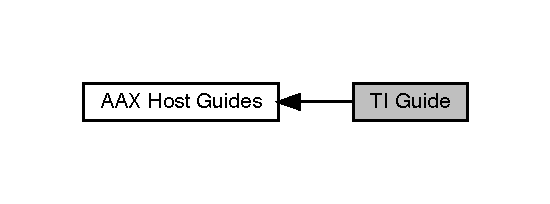
\includegraphics[width=264pt]{a00832}
\end{center}
\end{figure}
